\documentclass[]{article}
\usepackage{lmodern}
\usepackage{amssymb,amsmath}
\usepackage{ifxetex,ifluatex}
\usepackage{fixltx2e} % provides \textsubscript
\ifnum 0\ifxetex 1\fi\ifluatex 1\fi=0 % if pdftex
\usepackage[T1]{fontenc}
\usepackage[utf8]{inputenc}
\else % if luatex or xelatex
\ifxetex
\usepackage{mathspec}
\usepackage{xltxtra,xunicode}
\else
\usepackage{fontspec}
\fi
\defaultfontfeatures{Mapping=tex-text,Scale=MatchLowercase}
\newcommand{\euro}{€}
\fi
% use upquote if available, for straight quotes in verbatim environments
\IfFileExists{upquote.sty}{\usepackage{upquote}}{}
% use microtype if available
\IfFileExists{microtype.sty}{%
\usepackage{microtype}
\UseMicrotypeSet[protrusion]{basicmath} % disable protrusion for tt fonts
}{}
\usepackage[margin=1.25in]{geometry}
\usepackage{color}
\usepackage{fancyvrb}
\newcommand{\VerbBar}{|}
\newcommand{\VERB}{\Verb[commandchars=\\\{\}]}
\DefineVerbatimEnvironment{Highlighting}{Verbatim}{commandchars=\\\{\}}
% Add ',fontsize=\small' for more characters per line
\newenvironment{Shaded}{}{}
\newcommand{\KeywordTok}[1]{\textcolor[rgb]{0.00,0.44,0.13}{\textbf{{#1}}}}
\newcommand{\DataTypeTok}[1]{\textcolor[rgb]{0.56,0.13,0.00}{{#1}}}
\newcommand{\DecValTok}[1]{\textcolor[rgb]{0.25,0.63,0.44}{{#1}}}
\newcommand{\BaseNTok}[1]{\textcolor[rgb]{0.25,0.63,0.44}{{#1}}}
\newcommand{\FloatTok}[1]{\textcolor[rgb]{0.25,0.63,0.44}{{#1}}}
\newcommand{\CharTok}[1]{\textcolor[rgb]{0.25,0.44,0.63}{{#1}}}
\newcommand{\StringTok}[1]{\textcolor[rgb]{0.25,0.44,0.63}{{#1}}}
\newcommand{\CommentTok}[1]{\textcolor[rgb]{0.38,0.63,0.69}{\textit{{#1}}}}
\newcommand{\OtherTok}[1]{\textcolor[rgb]{0.00,0.44,0.13}{{#1}}}
\newcommand{\AlertTok}[1]{\textcolor[rgb]{1.00,0.00,0.00}{\textbf{{#1}}}}
\newcommand{\FunctionTok}[1]{\textcolor[rgb]{0.02,0.16,0.49}{{#1}}}
\newcommand{\RegionMarkerTok}[1]{{#1}}
\newcommand{\ErrorTok}[1]{\textcolor[rgb]{1.00,0.00,0.00}{\textbf{{#1}}}}
\newcommand{\NormalTok}[1]{{#1}}
\usepackage{longtable,booktabs}
\usepackage{graphicx}
\makeatletter
\def\maxwidth{\ifdim\Gin@nat@width>\linewidth\linewidth\else\Gin@nat@width\fi}
\def\maxheight{\ifdim\Gin@nat@height>\textheight\textheight\else\Gin@nat@height\fi}
\makeatother
% Scale images if necessary, so that they will not overflow the page
% margins by default, and it is still possible to overwrite the defaults
% using explicit options in \includegraphics[width, height, ...]{}
\setkeys{Gin}{width=\maxwidth,height=\maxheight,keepaspectratio}
\ifxetex
\usepackage[setpagesize=false, % page size defined by xetex
unicode=false, % unicode breaks when used with xetex
xetex]{hyperref}
\else
\usepackage[unicode=true]{hyperref}
\fi
\hypersetup{breaklinks=true,
bookmarks=true,
pdfauthor={},
pdftitle={},
colorlinks=true,
citecolor=blue,
urlcolor=blue,
linkcolor=magenta,
pdfborder={0 0 0}}
\urlstyle{same} % don't use monospace font for urls
\setlength{\parindent}{0pt}
\setlength{\parskip}{6pt plus 2pt minus 1pt}
\setlength{\emergencystretch}{3em} % prevent overfull lines
\setcounter{secnumdepth}{0}
\date{}
\usepackage{color}

\usepackage{fontspec}

\usepackage{setspace}

\usepackage{graphicx}

\definecolor{grey}{rgb}{0.5,0.5,0.5}

\usepackage{titling}


\usepackage{titlesec}
\newcommand*{\justifyheading}{\raggedleft}
\titleformat{\chapter}[display]
  {\normalfont\huge\bfseries\justifyheading\hrule\color{grey}}{\chaptertitlename\ \thechapter}
  {20pt}{\Huge}
\titleformat{\section}
  {\normalfont\Large\bfseries\justifyheading\hrule\color{grey}}{\thesection}{1em}{}


\usepackage{blindtext}
\usepackage{textcomp}

\makeatletter
\let\old@rule\@rule
\def\@rule[#1]#2#3{\textcolor{blue}{\old@rule[#1]{#2}{#3}}}
\makeatother

\let\stdsection\section
\renewcommand\section{\newpage\stdsection}




\doublespacing
\begin{document}
\setcounter{page}{1}
    \begin{center}
        \vspace*{1cm}
        
        \Huge
        \textbf{Timing and hippocampal information processing}
        
        \vspace{0.5cm}
        \LARGE
        
        
        \vspace{1.5cm}
        
        \textbf{Gregory Hale}
        
        \vfill
        
        A thesis presented for the degree of\\
        Doctor of Philosophy
        
        \vspace{0.8cm}
        

        
        \Large
        Department of Brain and Cognitive Sciences\\
        Massachusetts Institute of Technology\\
        USA\\
        January 12, 2015
        
    \end{center}
\newpage

{
\hypersetup{linkcolor=black}
\setcounter{tocdepth}{3}
\tableofcontents
}
\section{Abstract}

This thesis is about timing and information coding in the hippocampus.
In Chapter 1 we examine the timing of information coding in populations
of place cells - single neurons in the hippocampus that fire action
potentials at preferred locations in space. These neurons also exhibit a
surprising degree of coordination in time. In rats, when a series of
neurons are activated in turn by exploration of an environment, the same
sequence of spiking reappears spontaneously in sleep and as the rat
pauses to groom or eat. The sequences are sped up 10 times relative to
the sequence experienced on the track, but they preserve nearly perfect
time order. Zooming in, neurons' spikes during running are also tightly
organized into 10x-accelerated miniature versions of the macroscopic
sequence. This coordination is achieved with the help of a native
oscillation in the hippocampus called the \emph{theta rhythm}, and is
thought to be an important piece of the evolving story of how the
hippocampus encodes and remembers spatial information. In 2009 it was
discovered that the theta oscillation isn't synchronized across the
entire hippocampus, but instead looks more like a traveling wave, with
different parts of the hippocampus reaching the peak at different points
in time.

We set out to measure whether or not the traveling nature of the theta
oscillation has a desynchronizing effect on place cell spiking
sequences. We recorded from many place cells at once, some of them close
together experiencing the same oscillation, some far apart living in
different `time zones'. To our surprise, spikes remain tightly aligned
in distant groups of cells, replaying spatial sequences that are less
than one hundredth of a second off in their synchrony. That neurons
millimeters apart from each other can be so well coordinated lends more
evidence to the hypothesis that sequence replay is fundamental to
hippocampal information encoding. It opens more questions about how this
sequential spiking is achieved and how it is used by other parts of the
brain, which connect selectively with different hippocampal `time
zones'.

In Chapter 2, we discuss the development of ArtE, a tool for collecting
place cell sequence spiking from running rats and analyzing it in real
time. Typically this data is analyzed after the experiment has ended.
The goal for ArtE is to detect sequence replay events as they happen, so
that we can design experiments around closed-loop manipulations, for
example, rewarding the rat for expressing replay of one part of the
track and not the other part, and measuring the impact of biased replay
on behavior and on the information-carrying properties of place cells.
We take a fairly deep dive into the technical details of the
implementation of the tool, as well as a deep dive into Haskell, the odd
and wonderful programming language ArtE is written in.

Chapter 3 details a serendipitous finding that spiking activity in the
retrosplenial cortex reverts to a sleep like state in rats consuming
large rewards on mazes. The timing of these slow-wave sleep like
episodes is strictly limited to the times when the hippocampus undergoes
a similar transition, to a mode of spiking tightly associated with
slow-wave sleep.

We tie these topics together with a final discussion of the potential
role of population coordination in the encoding of spatial information,
the necessary next steps in connecting this activity with cortical
processing, and the recent advances in electrodes, imaging techniques,
and real time processing that will help us take these next steps.

To maximize the usefulness of this work, where possible, the supporting
data are available on Amazon S3 under a Creative Commons ShareAlike
license, and the source code is available at
\href{http://github.com/imalsogreg/RetroProject}{github.com/imalsogreg/RetroProject}
under BSD3. For those considering using this data in their own studies,
note that there are more peculiarities about the recording setup than we
could possibly enumerate, and it would be impossible to predict whether
these would confound your analyses. So we can not recommend basing new
papers on these data alone. However, the data may be extremely valuable
in pilot studies or as supplemental or confirmatory material. Both the
code and the data format may evolve as we prepare manuscripts or
accommodate cleanup requests from other research groups. Please check
the README.md and CHANGELOG.md at
\href{http://github.com/imalsogreg/RetroProject}{github.com/imalsogreg/RetroProject}
for updates in this regard. The source code for the ArtE backend is
hosted at
\href{http://arte-ephys.googlecode.com}{arte-ephys.googlecode.com} under
GNU GPL-v3, and the source code for the Bayesian decoder is at
\href{http://github.com/imalsogreg/arte-ephys}{github.com/imalsogreg/arte-ephys}
under BSD3. I have cut a release called \emph{thesis2014} for the
purpose of checking the results presented in this thesis against the
exact code used to generate them. If you find errors, please get in
touch.

\subsection{Dedication}

This work would not have been possible without the consistent support of
my family, especially my wife, who can relate directly to the experience
of writing a PhD thesis. I would also like to extend my sincerest thanks
to my advisor, Matthew Wilson, whose patience, understanding, and
principles played an enormous role in my development as a scientist. To
Hector, Denise, BCS2006 classmates and the rest of my support network,
Thank You!

\section{Coordinated information coding in a desynchronized network}

\subsection{Abstract}

Brain areas involved in mnemonic and spatial processing are locked to an
underlying 8-12 Hz oscillation known as the theta rhythm. In addition to
pacing cell excitability, theta influences spatial information
processing by organizing the timing of place cell ensembles into
temporally precise ``theta sequences". Theta rhythms were recently shown
to have substantial timing offsets across the hippocampal medial-lateral
axis {[}1{]}. We sought to determine the impact of theta timing offsets
on theta sequences - are sequences in distant groups of cells offset in
time, or synchronized?

We recorded from populations of place cells and measured theta sequence
properties with Bayesian position reconstruction and pairwise timing
correlations. Along the CA1 medial-lateral axis, we estimate theta
sequences to be synchronized to within 5 ms per millimeter, despite a
time offset in theta on the order of 13 ms per mm. This suggests that
the timing of bulk spike rate can be decoupled from the underlying
information carried in those spikes.

This observed information synchrony in the context of desynchronized
excitation provides a constraint for future models of fast-timescale
position coding. Current models of theta phase precession all make use
of the local phase of theta and would have predicted that theta
sequences would be desynchronized by desynchronization in the underlying
theta. We put forward two explanatory models that could account for our
results and propose experiments that could distinguish between them.
Future work will help us determine whether the traveling theta wave
results in output structures connected to different parts of CA1
receiving those inputs at different times, and what role the synchrony
of CA1 encoding has on that temporally structured communication.

\subsection{Introduction}

\subsubsection{CA1 place cell excitation is timed by 10Hz oscillation -
theta rhythm}

In many brain areas associated with spatial learning {[}2--5{]} and
episodic memory {[}6--8{]}, neural activity is modulated by a 7-12 Hz
oscillation called the theta rhythm {[}9--11{]}. The influence of the
theta oscillation on spatial and mnemonic information processing has
been appreciated at two levels. On the global level, theta is thought to
coordinate activity between connected brain regions {[}1,12--15{]}.
Locally, theta shapes the fine-timescale properties of information
coding within brain areas, by way of theta phase precession {[}16{]}.

\subsubsection{Theta sequences}

Place cells spike at precise phases of theta that depend on where a rat
is within the place field. The spikes at the beginning of the place
field occur at early phases and spike near the end of the field occur at
later phases {[}16{]}. This led to the prediction that a collection of
cells with partly overlapping fields will fire in a strict order
according to the relative positions of the place fields {[}17,18{]}.
Later these sequences were observed directly in large groups of
simultaneously recorded neurons {[}19--21{]}. Interestingly, the tight
temporal alignment of place cells in theta sequences is greater than the
precision with which individual cells align their spikes to the theta
oscillation {[}19{]}.

Our goal is to understand how the brain processes information during
navigation and how that processing leads to later recall. Although we
can determine a rat's position very precisely using only firing rate
information from place cells {[}22{]}, it has not been established that
this is how the rest of the brain interprets hippocampal spiking
{[}23{]}. The conspicuously precise sequential ordering of place cell
ensembles beyond the temporal resolution of a rate code suggests these
sequences as not just a means for adding a bit more accuracy to an
estimate of one's current position {[}24{]} but a potentially
fundamental aspect of limbic information processing {[}25,26{]}.

Understanding the mechanism of theta sequence generation will be
important for reasoning about their interactions with other brain areas
and possible functional roles. There is not agreement about their
mechanism though (in fact very little is known about the origins of
spatial properties of cells throughout the limbic circuit), but
hypothesized models fall into three camps that emphasize either
oscillatory interference, Hebbian phase sequences, or sub-threshold
receptive fields.

The oscillatory interference model suggests that place cells oscillate
at a rate slightly faster than theta measured in the LFP, and that the
interference pattern of the two oscillators is a more complex waveform
with local peaks that precess with respect to the LFP theta and a low
frequency envelope that determines the length of the place field (for
details, see {[}16{]}). This theory is supported by intracellular
recordings of the soma and dendrites of hippocampal place cells, which
do indeed produce precessing spikes in response to inputs presented at
different frequencies {[}27{]}, and which show some signs of oscillatory
acceleration during movement through the place field {[}28{]}. The main
weakness of the model is that the oscillations discussed are purely
temporal and their interaction is expected to carry on at a constant
rate regardless of an animal's speed, but in reality phase precession
aligns with the animal's location within a place field better than it
does with time spent in a place field {[}16{]}. Tweaking the model to
match this observation requires a strong correlation between running
speed and theta frequency that isn't seen empirically {[}16,29,30{]}. An
additional problem for the oscillatory interference model comes from the
observation that phase precession continues after the cessation of a
brief silencing of the hippocampus {[}31,32{]}.

Hebbian phase sequences {[}33{]} are sets of assemblies of cells that
excite one another in a feed-forward synaptic chain. One constellation
of neurons preferring location \(x\) on the track collectively synapse
on the population preferring \(x+\delta\), and so on, causing a rapid
succession of cell assemblies, initiated by the sensory details of the
current physical location and terminated by the subsequent surge of
theta-rhythmic inhibition, to sweep out a theta sequence ahead of the
rat, much as neurons in the HVC seem to unfold in collateral synfire
chains during song production in the finch {[}34,35{]}. For the
hippocampus though, this model suffers when it comes to producing theta
sequences in two-dimensional arenas. Empirically, theta sequences sweep
forward in the direction that the rat is facing. The hippocampus would
somehow need to unmask selectively the synapses that activate a
West-bound sequence of assemblies when the rat is headed West and a
North-east bound sequence when the rat is headed North-east, etc. At
this point it becomes hard to imagine how such specific matrices of
connections could be formed and subsequently selected on a
moment-to-moment basis, although there is some work involving grid cells
{[}5{]} that may make this more feasible {[}36{]}.

The third model, called the rate-to-phase model, considers CA1 spike
timing as an interaction between an excitatory input that ramps up
smoothly with spatial location in a place field, on one hand, and the
temporally oscillating inhibitory effect of theta, on the other
{[}37{]}. For any given position in the place field, spikes are fired at
the moment when inhibition drops below the excitation associated with
that location. Progress in the field and greater excitation means less
waiting for inhibition to drop to meet the excitation level, and thus
earlier phases. This model directly references space to achieve phase
precession, and therefore naturally copes with the finding that phase
precession goes according to distance traversed within a field than time
spend in a field. Because neither this model nor the phase sequence
model involve previous reverberatory activity, they are both compatible
with the transient inhibition studies {[}31,32{]}.

One thing that is unclear about the rate-to-phase model is where these
hypothesized excitatory ramp comes from. The ramping excitation is
strictly required to be monotonically increasing; if it were bell-shaped
like the place fields of some place cells, we would expect to see a
pattern of phase precession followed by phase procession back to late
phases, but this does not happen. Additionally, there is no known
mechanism that could smooth the summed inputs to CA1 into such a flat
ramp; indeed the main inputs to CA1 are themselves theta-rhythmic
signals.

Another parameter the rate-to-phase model leaves abstract is the nature
of the rhythmic inhibition. It it the somatic inhibition on place cells,
the trough of dendritic excitation, the peak spiking phase of a
particular class of interneuron? The model works well for accounting for
phase precession through a single field without committing to a
particular concrete source of theta, but we will need more information
as we try to predict higher-order features, for example, the behavior of
pairs of cells that for whatever reason are not receiving identical
inhibitory inputs.

Theta phase precession has been observed in CA3 {[}16{]}, dentate gyrus
(DG) {[}17{]}, medial prefrontal cortex {[}38{]}, ventral striatum
{[}39{]}, entorhinal cortex (EC) layer II (but not layer III) {[}40{]}
and the subiculum {[}41{]}, as well. Whether phase precession organizes
cells within a given area into theta sequences or supplies some other
form of ensemble organization, we refer to this as a 'local' role for
theta: a set of timing constraints that single cells or small groups
must obey perhaps for temporal coding or time-sequence coding.

\subsubsection{Communication through coherence}

At the same time, there is an effort to understand the firing properties
of parts of the hippocampus in terms of information flow through a
hierarchy of structures with unique functions, similar to the work being
done in the visual circuit {[}42{]}. Here, theta is hypothesized to have
a more global role in facilitating the transmission of information
between areas. Hippocampal and prefrontal cortical theta oscillations
become coherent at times when maze navigation needs to refer to the
contents of working memory {[}12{]}, and this coherence is reflected in
the spike times of both hippocampal and prefrontal neurons {[}43,44{]}.
Spatially restricted bouts of gamma oscillations in somatosensory cortex
are modulated by hippocampal theta phase {[}13{]}, providing an
interesting link to the large literature surrounding cortical gamma
oscillations. More direct evidence on the role of theta in pacing gamma
oscillations comes from Colgin et. al. {[}14{]}, who showed that in CA1,
high-frequency gamma oscillations occur primarily at the peak CA1
spiking phase and are coherent with simultaneous high-frequency gamma
oscillations in entorhinal cortex; while low-frequency gamma is
strongest about 90° earlier and is coherent with low-frequency gamma in
hippocampal CA3. Based on this Colgin argues that selective theta
coherence tunes CA1 to communicate preferentially with one input source
or the other.

A related global role for theta attributes specific sorts of information
processing to different theta phases; namely that the phase associated
with peak entorhinal cortex spiking is responsible for encoding new
information and the phase associated with input from CA3 is responsible
for memory retrieval {[}45{]}.

\subsubsection{Tension between hypothesized roles in gating
communication channels and encoding}

These two roles for theta oscillations are difficult to unify, because
they make conflicting demands on the details of how neurons interact
with the oscillation. If a cell is meeting the timing requirements of
selective communication with varying brain areas, can it simultaneously
be aligning its spikes fall at progressively earlier theta phases when a
rat moves through the cell's place field?

One model suggests that meeting these requirements simultaneously
results in strict relationships between global and local phenomenon, and
that we get scientific findings from this 'for free'. Fries {[}46{]}
extrapolates from Colgin's {[}14{]} work and concludes that early phases
of theta in CA1 processes cortical information about the current state
of things, and later phases use the modeling capabilities of CA3 to
extrapolate into the future. This model is appealing when observing the
shape of theta sequences in place cell ensembles; they begin near the
rat's current position and sweep quickly out ahead of him, repeating
this at every theta cycle. And it accords with the notion of the
entorhinal cortex as a sensory structure (being upstream of the
hippocampus), and Marr's notion of the CA3 as a pattern extrapolator
{[}47{]}.

Can we account for the theta-locked spike timing of limbic circuit
structures in terms of their anatomical ordering? Here things become
more difficult. Mizuseki et. al. {[}48{]} show that cells in different
structures prefer to fire at different theta phases that bear little
resemblance to the sequence implied by a synaptic traversal of the
circuit. Rather than EC-Layer II \(\rightarrow\) DG \(\rightarrow\) CA3
\(\rightarrow\) CA1 \(\rightarrow\) EC-Layer V (the synaptic pathway of
the major hippocampal excitatory circuit), CA3 principal cells to spike
90° earlier than EC-Layer II principal cells. Additionally, spikes of
CA1 neurons occur at the opposite phase from that of their peak
dendritic excitation {[}10,49{]}. This phenomenon is acceptable to the
global account of theta; it allows for the opening of 'temporal windows'
of processing between sequential anatomical processing stages {[}48{]}.
But it is at odds with intuitive and formal {[}49,50{]} models of the
fine timescale spiking of place cells, which we expect to follow behind
their inputs by conduction delays and synaptic delays. The empirical
timing relationships are much longer {[}48{]}.

Colgin et. al. present data in support of a model associating particular
phases of the theta oscillations of CA1 with the opening of specific
communication channels to either CA3 or the entorhinal cortex {[}14{]}.
The tension between theta's local and global roles is apparent here, as
well. To the extent that CA3-CA1 and entorhinal-CA1 communication is
limited to narrow windows of theta phase. Contrary to this, place coding
in CA1 involves a smooth transition through cell ensembles that extends
over much of the theta cycle {[}19,20{]}.

\subsubsection{Theta as traveling wave, excitatory time offsets over
hippocampal CA1}

Lubenov and Siapas {[}1{]} presented a novel finding about the nature of
the theta oscillation itself. Using large grids of tetrodes carefully
positioned a uniform distance from the hippocampal cell layer, and
sampling a large extent of the length of the hippocampus, they showed
that the theta rhythm is not synchronous within hippocampal CA1.
Instead, theta at the septal pole of CA1 are advanced in phase, theta in
more posterior parts of CA1 are phase delayed, and theta measured in
between has a graded delay. The combined activity of these delays
resembles a traveling wave with a peak of excitation that 'moves' down
the hippocampal long axis once for every cycle of theta. These findings
were extended beyond dorsal hippocampus to the entire length of CA1 by
Patel et. al. {[}51{]}.

By fitting a traveling wave model over the pattern of theta offsets
observed over many tetrodes, Lubenov and Siapas were able to extract
parameters that can be used in concrete hypotheses. The characteristics
of the wave vary from cycle to cycle, but tend to have a spatial
wavelength of 12mm, a wave-front speed of 75 mm/sec and a preferred
direction about half way between the medial-lateral axis of the skull
and the septo-temporal axis of the hippocampus. Based on these
parameters {[}1{]} and our own LFP measurements, we can establish the
mean expected time offset along the direction of wave propagation as
\(1/\nu\), 12.8 \(\pm\) 3.2 ms per mm.

\subsubsection{Theta sequences: locally paced or globally synchronized?}

The view of theta as a traveling wave will need to be factored in to any
future models that unify the local and global roles for theta, because
it has interesting implications in both areas. With theta mediating
information transmission to and from CA1, how will those inputs and
outputs cope with the fact that the window of receptivity is a moving
target? Is it acceptable that structures receiving inputs from one part
of CA1 will see maximum activity at a different time from structure
receiving inputs from another part of CA1 - and could this sequencing
actually be useful?

How does this fit when we zoom in from talking about bulk spiking rates,
to the level of information-carrying single spikes at the local level?
If theta phase precession conforms to the anatomically sweeping of peak
excitation, then theta sequences composed of sets of cells from
different regions of CA1 would be similarly offset in time. The periodic
replay of spatial sequences would begin slightly earlier in septal CA1
ensembles, and ensembles near intermediate CA1 would begin the same
sequence about 45ms later, with ensembles further posterior starting
later still. This time shifting may seem to complicate attempts to
square theta sequences with anatomical communication. However, it leads
to an interesting prediction: that local regions of hippocampus begins a
representation trajectory at offset times. Because of this, a downstream
structure observing a snapshot of the spiking activity across the whole
hippocampus would see different parts of the track encoded at different
anatomical locations. Or as Lubenov and Siapas put it, the hippocampus
at any instant would not represent a point in space, but a linear span
in space {[}1{]}.

Alternatively, theta sequences may not conform to the timing offsets
suggested by the traveling theta wave, and the encoded information may
be temporally synchronized over large anatomical distances, despite the
presumed timing differences in their underlying drive. This scenario
presents a very different picture to downstream structures - one in
which bulk spike output of the hippocampus goes as a traveling wave, but
the information content within it is coherent, and the entire structure
does agree to a single point on the track at any instant.

We set out to measure the timing relationship between theta waves and
place cell sequences in order to address this one question among many
others aimed at unifying the local and global roles for theta in timing
spikes. We characterized the impact of spatial tuning and anatomical
distance on the co-firing of pairs of place cells, as well as the timing
relationships of population-encoded trajectories recovered from
anatomically distinct groups of cells, both across CA1 and between CA1
and CA3. We found that in most cases, timing offsets in theta sequences
were significantly more synchronized than the temporally offset
excitatory waves that modulate them. We suggest that information
synchrony may be decoupled from the mechanisms that modulate excitation.
This decoupling could be achieved in a trivial way, by stipulating that
phase precession begins and ends according to an underlying source that
is in fact synchronized across hippocampus; or it could be achieved
through an active mechanism that supplies extra excitation to the
regions that would otherwise be temporally delayed by the traveling
theta wave.

\subsection{Materials \& Methods}

\subsubsection{Subjects}

All procedures were approved by the Committee on Animal Care at
Massachusetts Institute of Technology and followed US National
Institutes of Health guidelines. Tetrode arrays were assembled and
implanted according to the procedure in Nguyen et. at. {[}52{]} and
Kloosterman et. al {[}53{]}. We made several modifications to the
materials and procedures to improve our multi-cell sampling. First, we
glued several hundred half-inch pieces of 29 gauge and 30 gauge
hypodermic tubing into rows about 6 mm long, then stacked and glued the
rows together to form a honeycomb patterned jig, for organizing the
tetrode guide-tubes that would eventually inhabit the microdrive.
Second, we developed the ArtE recording system (detailed in Chapter 2)
to run in parallel with our usual usual tetrode recording rig. The
broader goals of the ArtE project are to enable real-time data analysis
and feedback, but in this experiment we used it merely to increase the
number of simultaneously recorded tetrodes.

\subsubsection{Single-unit tetrode recording}

Microdrive arrays were implanted with the center of the grid of tetrodes
overlying dorsal CA1 (A/P -4.0, M/L 3.5), spanning 3 mm of hippocampus
in the septo-temporal dimension and 1.5 mm proximo-distal. Tetrodes were
lowered into the pyramidal cell layer of CA1 over the course of 2 to 3
weeks and left there for several more weeks of recording. We sought to
maximize the number of neurons recorded and to minimize
within-experiment drift, so we closely tracked the shape of sharp wave
ripples (which undergo characteristic changes during approach to the
cell layer) and later the amplitudes of burgeoning clusters. If either
of these factors changed overnight to a degree greater than expected,
the tetrode was retracted by 30 - 60 micrometers.

\subsubsection{Behavioral training}

Behavioral training began when nearly all tetrodes exhibited separable
spike clusters, and consisted of rewarding rats for simply running back
and forth on a curved 3.4 meter linear track, or running continuously
clockwise on a 3.4 meter long circular track, with rewards given for
every 360 degrees of running for the first 3 laps and for every 270
degrees thereafter. Food deprivation began one or two days prior to the
beginning of acquisition, with rats receiving 30 grams of food per day,
adjusted up or down depending on the rat's motivation to run and level
of comfort (assessed by the amount sleep taken before the running
session). The target food-deprived weight was 80\% of free-feeding
weight, but we rarely achieved this without disrupting the sleep of the
animals, so body weights tended to be 90\% of the free-feeding weight or
more, especially after rats learned the simple rules of the task. We
provided rewards throughout training (200-500 milligrams of wetted
powdered rat chow per lap), to encourage the long stopping periods
during which awake replay can be observed {[}54{]}. Under these
conditions, rats run for about 20 laps or 30 minutes before becoming
satiated and ignoring rewards.

\subsubsection{Electrophysiological Characterization}

Spikes and local field potentials were voltage buffered and recorded
against a common white-matter reference, at 32 kHz and 2kHz
respectively, and position was tracked at 15 Hz through a pair of
alternating LED's mounted on the headstage, as in Davidson et. al.
{[}21{]}. Spikes were clustered manually using the custom program,
xclust3 (M.A.W.). Place fields were computed for each neuron as in Zhang
et. al. {[}55{]}, by partitioning the track into 50 to 100 spatial bins,
and dividing the number of spikes occurring with the rat in each spatial
bin by the amount of time spent in that spatial bin, in each case only
counting events when the rat was moving at least 10 cm/second around the
track. Direction of running was also taken into account, allowing us to
compute separate tuning curves for the two directions of running, which
we label 'outbound' and 'inbound'.

To characterize the phase differences among tetrodes in CA1, a simple
spatial traveling wave model was fit to the theta-frequency filtered LFP
signals and the theta-filtered multiunit firing rate in turn, as in
Lubenov and Siapas {[}1{]}.

\subsubsection{Theta sequences}

Two complementary techniques were used to assess the relationship
between phase offsets between tetrodes and timing offsets in spatial
information encoding. First, in CA1-only recordings, a pairwise
regression was performed similar to that in Dragoi and Buzsaki {[}18{]},
measuring the dependence of short-timescale peak spike time differences
on the distance between the peaks of that pair's place fields. We added
a second independent variable to this regression: the anatomical
distance between each pair of place cells. The result is a model that
predicts the average latency between any pair of cells, given that
pair's place fields, that pair's anatomical separation, and the
parameters of the traveling wave pattern of phase offsets.

Second, Bayesian stimulus reconstruction {[}55{]} was carried out
independently using place cells from three groups of tetrodes at the
most septal end, the middle, or the most temporal end of the 3mm
recording grid. Unlike the case for large populations of neurons,
reconstructions from smaller anatomical subsets are considerably more
noisy and do not reliably yield theta sequences. Session-averaged theta
sequences were recovered by aligning the reconstructed position
according to a shared theta phase and the rat's position on the track at
that time. In both raw and session-averaged reconstruction cases, 2d
autocorrelograms were taken to quantify the time-delay and space-delay
between pairs of tetrode subgroups.

\subsection{Results}

\subsubsection{Theta phase spatial properties and timing offsets: 13ms
delay per mm}

We first characterized the timing of the local-field potential (LFP)
theta rhythm within a \textasciitilde{}3mm long, 1.5mm wide strip dorsal
CA1, in electrodes embedded near the pyramidal cell layer. A traveling
wave model was fit to the theta-filtered and Hilbert-transformed signals
from 16 to 24 tetrodes, in 0.25 second segments, resulting in a
time-course of traveling theta wave parameters (Figure 1). We focus on
the parameters that characterize the desynchronization: spatial
wavelength, wave propagation direction, and temporal wavelength.

\begin{figure}[htbp]
\centering
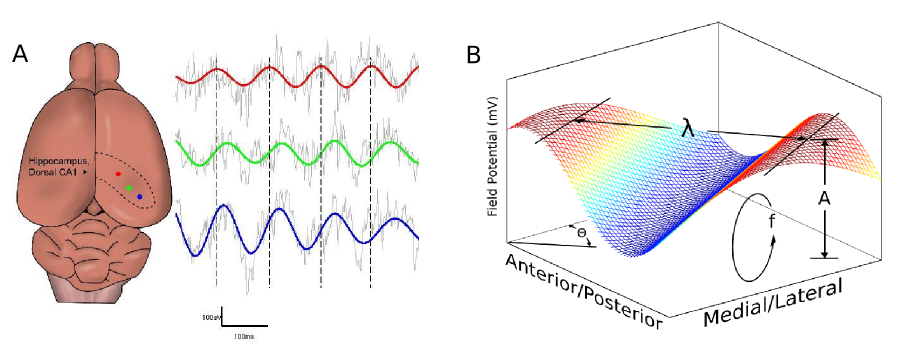
\includegraphics{./finalFigs/brainAndModel.png}
\caption{\textbf{Theta is desynchronized within CA1.} \textbf{A.} The
rat hippocampus (left dashed region) occupies a large of the cortex.
Three example recording sites (red, green and blue points) experience
different phases of theta oscillation in the local field potential
(right). On average, recording sides experience increasing phase delay
as they move lateral and posterior {[}1{]}. Raw LFP traces (in grey)
exhibit theta oscillations and gamma oscillations that depend on
electrode depth. Filtered theta components shown in red, green, and
blue. \textbf{B.} The pattern of phase-offsets in LFP recordings was fit
by a traveling wave model in 0.25 second segments. The traveling wave
model consists of parameters for wave direction (\(\theta\)), spatial
wavelength (\(\lambda\)), amplitude (A), temporal frequency (f), and
phase offset (\(\varphi\), not shown).}
\end{figure}

These parameters vary on a short timescale but are fairly consistent
between animals when averaged across time. Theta frequency during
running varies from 8.2 Hz \(\pm\) 0.5 (mean \(\pm\) standard
deviations). The spatial wavelength is 6.3 mm \(\pm\) 3.6 after removal
of outliers, and the dominant propagation direction is 18° anterior to
the medial-lateral axis. Surprisingly, the fit of the model was not
higher during running than during stopping periods when theta amplitude
is low, suggesting that traveling waves are a broad enough family to fit
many patterns of data (in fact, a traveling wave model will perfectly
fit a set of perfectly synchronized oscillators; the spatial wavelength
in this case would be infinity). As was previously reported {[}1{]},
proximity of tetrodes to the pyramidal cell layer obscures the LFP
measurement of the traveling wave, so we primarily rely on previously
reported wave parameters.

\begin{figure}[htbp]
\centering
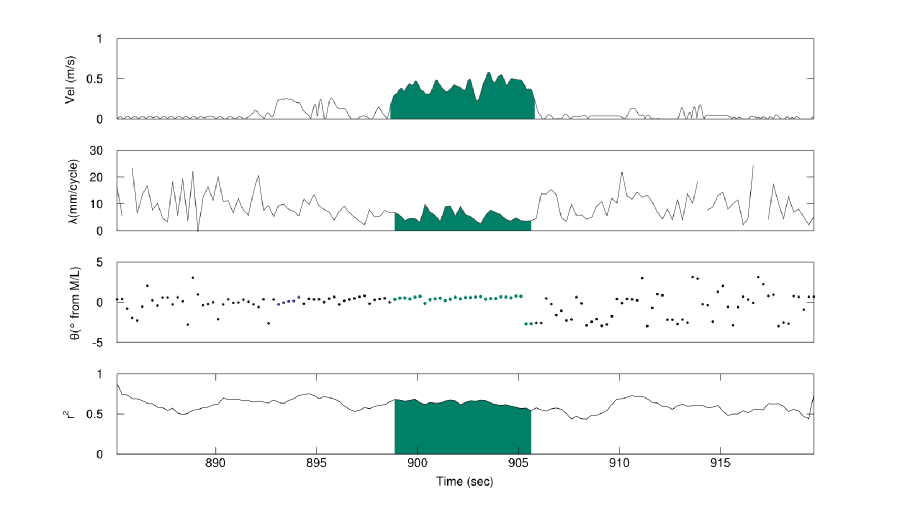
\includegraphics{./finalFigs/waveTimecourse.png}
\caption{\textbf{Theta traveling wave parameters can be stable over time}.
\textbf{A.} About of running (green time window, top panel) elicits a
stabilization of the traveling wave fit to theta. During this time, the
spatial wavelength varies between 3 and 10 mm, and wave direction
remains fairly constant about 18° anterior to the medial-lateral axis,
except for a brief direction flip near the end of the run. The fit of
the model to the data is not better during the running periods than the
stopping periods, although the variability in parameters during run is
lower, because the ability to record the traveling wave is lower when
the tetrodes are near the pyramidal cell layer {[}1{]}, as they were in
this case. \textbf{B.} The traveling wave velocity inverted gives a
wave-delay interval. In this dataset, the mean delay was 17.8 ms per mm
along the medial-lateral axis. Combining with studies optimized for
recording the LFP, the estimate is 12.8 ms per mm.}
\end{figure}

\subsubsection{Place cell pairs are synchronized across anatomical
space}

We directly measured the relationship between anatomical spacing and
spike timing in pairs of place cells. If two cells with the same place
field and phase precession profile are separated by a spatial interval
corresponding to a 13ms delay between theta peaks, two fast-timescale
timing relationships are possible. Either phase precession is locked to
to the local theta oscillation, and spikes from the cell 1mm
'downstream' with respect to the traveling wave will occur 13ms later
than those of the upstream cell (Figure 3). Alternatively, if phase
precession disregards the anatomical delays of theta phase, then spikes
from the two cells should fire roughly in synchrony. Other timing
relationships are possible of course, but it is not clear what they
would imply mechanistically.

\begin{figure}[htbp]
\centering
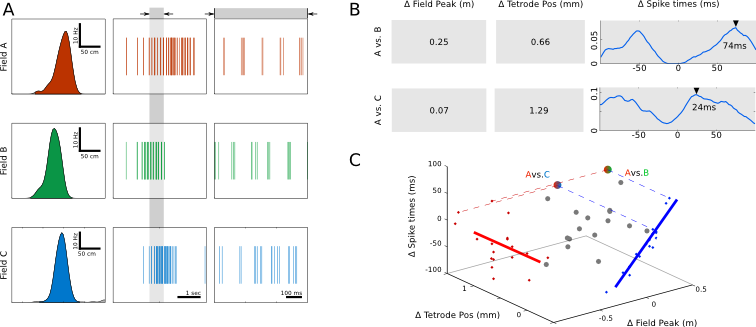
\includegraphics{./finalFigs/pairXCorr.png}
\caption{\textbf{Assessing the effect of tuning curves and anatomical location on spike timing.}
\textbf{A.} Three place cells with partly overlapping fields. Tuning
curves are plotted in the left column. In the center and right columns
are a raster plot of several seconds, and a several hundred millisecond
detail. \textbf{B.} Cell A's place field peak is 25 cm beyond Cell B's,
its anatomical position is 0.66 mm more lateral, and it tends to fire 74
ms later (the peak offset of the cross correlation of the two spike
trains). Cell A's place field peak is 7 cm beyond Cell C's, its
anatomical position is 1.29 mm more lateral, and it tends to fire 24 ms
later. \textbf{C.} A scatter-plot of all pairs of place fields (gray
dots), taking the peak time offset between the spike trains as a
function of both place field distance and anatomical distance.
Projecting all of the points to one axis shows the correlation between
field distance and time offset due to theta sequences (blue). Projecting
onto the other axis shows the much weaker correlation between anatomical
offset and timing offset (red).}
\end{figure}

These predictions can be generalized beyond cell pairs with perfectly
overlapping fields. Field separation will result in a timing shift due
to phase precession. The virtual speed of the rat encoded in theta
sequences is about 10 m/s, so a cell with a field peaking 0.5 meters
beyond that of another cell will tend to spike 50 ms later. If phase
precession is paced against the local theta, then anatomical separation
on the axis of the traveling wave should add to this delay linearly. We
can estimate the effects of place field spacing and anatomical spacing
on spike timing by linear regression (Figure 3).

\begin{figure}[htbp]
\centering
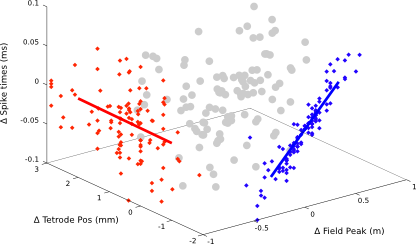
\includegraphics{./finalFigs/pairXcorrSummary.png}
\caption{\textbf{Field location is the primary determinant of spike time offsets.}
The scatter-plot of the previous figure, combining all cell pairs (gray)
from four recording sessions, considering timing offsets (z-axis) as a
function of both place field distance (right axis) and anatomical
distance (left axis). Projecting the points onto one axis shows a strong
correlation between field distance and timing offsets (blue) due to
theta sequences. Projecting onto the other axis shows the much weaker
correlation between anatomical offset and timing offsets (red).}
\end{figure}

Pooling cell pairs across rats, we estimate each meter of place field
distance to contribute 147.4 \(\pm\) 14.2 ms of delay and each mm of
anatomical spacing along the traveling wave axis contributing 0.7
\(\pm\) 3.3 ms, significantly less lower than the expected 12.8 ms per
mm (p \textless{} 0.05). In other words, place cells fire with temporal
delays that reflect spatial relationships on the track, and these
spiking events are tightly coordinated throughout the measured extent of
CA1 (about 3 mm).

\begin{longtable}[c]{@{}lllll@{}}
\caption{\textbf{Anatomical separation accounts for relatively little timing offset.}
Results of the regression analysis of the previous figure for each
recording session. In three of four rats, the isolated effect of
anatomical distance of time offsets is less than the 12.8 ms per mm time
delay of the theta wave. Pooling cell pairs into a single regression
results in a final estimate of 0.7 ms per mm. The effect of field
separation on the other hand is reliably in line with previous accounts
of theta sequences.}\tabularnewline
\toprule
Session & Anatomical (ms/mm) & Field (ms/m) & Offset (ms) & \# of
Pairs\tabularnewline
\midrule
\endfirsthead
\toprule
Session & Anatomical (ms/mm) & Field (ms/m) & Offset (ms) & \# of
Pairs\tabularnewline
\midrule
\endhead
Yolanda A & -7.0 \(\pm\) 13.9 & 101.2 \(\pm\) 20.0 & 7.3 \(\pm\) 11.3 &
31\tabularnewline
Yolanda B & -1.2 \(\pm\) 16.4 & 199.1 \(\pm\) 40.9 & 1.2 \(\pm\) 11.0 &
18\tabularnewline
Morpheus & 0.9 \(\pm\) 3.3 & 163.1 \(\pm\) 20.7 & -2.1 \(\pm\) 5.2 &
38\tabularnewline
Caillou & 18.6 \(\pm\) 12.8 & 198.1 \(\pm\) 25.1 & 6.4 \(\pm\) 7.9 &
19\tabularnewline
\textbf{Total} & \textbf{0.7 \(\pm\) 3.3} & \textbf{147.4 \(\pm\) 14.2}
& \textbf{-0.4 \(\pm\) 3.5} & \textbf{106}\tabularnewline
\bottomrule
\end{longtable}

\subsubsection{Ensemble theta sequences are synchronized}

To assess the impact of anatomical distance on spatial representations
from another angle, we turned to population decoding, which provides a
direct view of theta sequences as well as spontaneous spatial replay
events.

\begin{figure}[htbp]
\centering
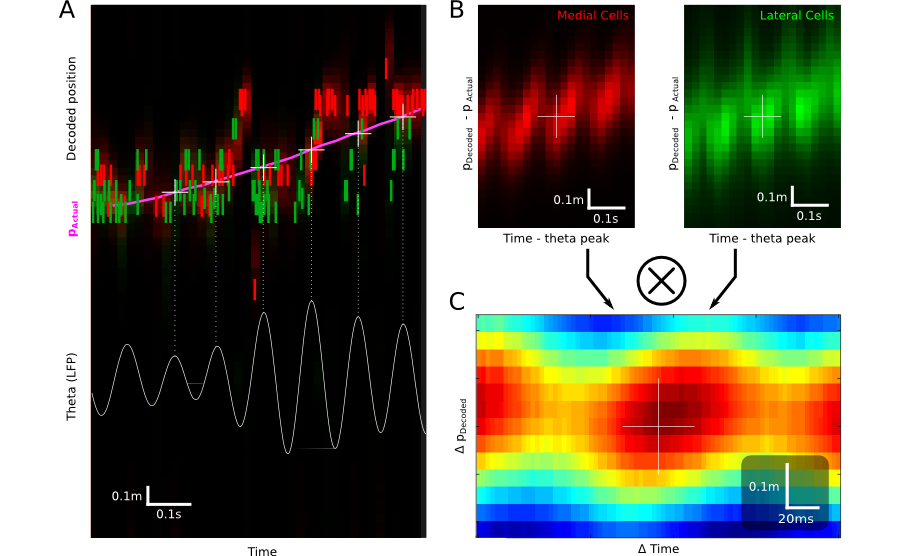
\includegraphics{./finalFigs/sequences.png}
\caption{\textbf{Reconstructed theta sequences in medial and lateral hippocampus}.
\emph{A:} One second of position decoding from neurons in medial (red)
and lateral (green) CA1. Theta sequences are bracketed by cycles of the
theta rhythm (white). \emph{B:} Triggered-average theta sequences from
medial (red) and lateral (green) position reconstructions. Triggers were
centered in time on theta peaks, and centered in position on the
physical track location of the rat at the time of the peak. \emph{C:}
Cross correlation between lateral and medial triggered average theta
sequences.}
\end{figure}

Within CA1, we partitioned cells into three groups according to the
tetrode they were recorded on, then discarded the middle group, leaving
two groups separated by a millimeter at their closest point, two
millimeters on average. We then reconstructed the rat's location twice,
once from each set of tetrodes, at a 15ms temporal scale suitable for
observing theta sequences. The division of tetrodes into independent
anatomical groups drastically degrades the appearance of ongoing theta
sequences, because the reconstruction process at such short timescales
requires input from a large number of neurons. But clear theta sequences
can be recovered by combining segments of the position reconstruction,
aligned in time by peaks of the theta rhythm, and in space by the rat's
current track position (Figure 5B).

\begin{figure}[htbp]
\centering
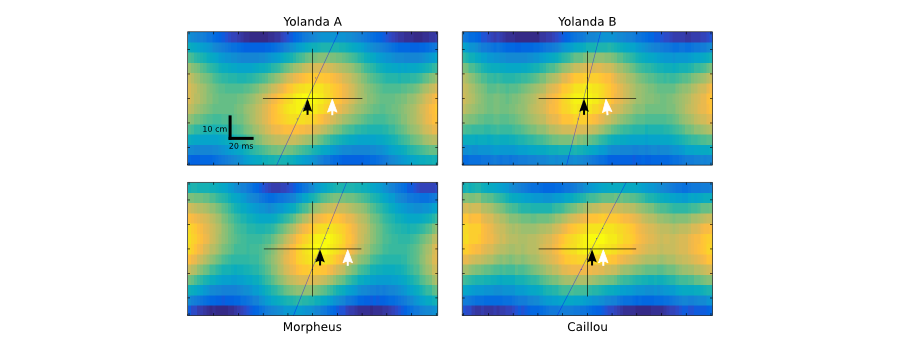
\includegraphics{./finalFigs/sequences_all.png}
\caption{\textbf{Theta sequence cross correlations for all recording sessions.}
The cross correlations between theta sequences computed from medial and
lateral place cell groups for each recording session. Diagonal streaks
across the origin indicate that theta sequences resemble one another
after a combination of time shift and position shift, but not a
time-shift alone. Black arrows: pure time shift between medial and
temporal cell groups. White arrows: time shift expected if theta
sequences are uniformly delayed by traveling theta wave.}
\end{figure}

We asked whether the reconstructed theta sequences are aligned with one
another in time by taking their two-dimensional cross-correlation
(Figure 4). A uniform delay of the theta sequence by time \(\delta\)
would appear as a diagonal streak that crosses the x axis at \(\delta\).
The peak of this cross correlation occurs when septal CA1 leads temporal
CA1 by 3.5 ms in time. We estimate the uniform delay that theta
sequences would incur in the lateral portion of the hippocampus by
multiplying the 12.8 ms/mm delay estimate by the mean inter-place cell
distance for each recording session. In this example, the mean spacing
between place cells is 1.05 mm along the medial-lateral axis, so a
simple delay would result in 13.44 ms. These statistics for each rat are
given in Figure 6 and Table 2. Observed time offsets are significantly
different from those expected by uniform time delay of the traveling
wave (p \textless{} 0.05).

In two of the recording sessions, although the cross correlation extends
through the origin, its center of mass is delayed. This pattern
indicates that lateral cells fire tend to fire later than medial cells,
but with a balanced advancement in encoded track location. Rather than
theta sequences being time delayed in lateral cells, the bulk of the
spiking involved in a theta sequence comes from medial hippocampus
first, and from lateral hippocampus slightly after, with the information
content between them closely coordinated. This pattern is in the
opposite direction in the two other recording sessions; indicating that
on average in those two sessions, lateral hippocampus place cells fire
more vigorously in the first half of theta sequences and medial
hippocampal place cells fire later. Collecting all of our datasets, we
do not find significant evidence to reject the null hypothesis that the
cross-correlation center of mass is at zero (p = 0.7030), but we suspect
that this is due to the low number of recording sessions and the
dependence of this measure on the number of place cells simultaneously
recorded.

\begin{longtable}[c]{@{}lllll@{}}
\caption{\textbf{Theta sequences are aligned in time.} Average and
minimum anatomical distances, along the direction of wave propagation,
between place cells in the two groups used for theta sequence decoding.
Expected time offsets are derived from the estimated wave delay times
the mean spacing. Offsets observed from the mean theta-sequence
cross-correlations are close to zero, suggesting that that distant theta
sequences are tightly synchronized.}\tabularnewline
\toprule
Session & Mean spacing (mm) & Min spacing (mm) & Expected offset (ms) &
Observed offset (ms)\tabularnewline
\midrule
\endfirsthead
\toprule
Session & Mean spacing (mm) & Min spacing (mm) & Expected offset (ms) &
Observed offset (ms)\tabularnewline
\midrule
\endhead
Yolanda A & 1.33 & 0.94 & 17.02 & -4.0\tabularnewline
Yolanda B & 1.30 & 0.94 & 16.64 & -3.0\tabularnewline
Morpheus & 2.27 & 1.47 & 29.06 & 6.0\tabularnewline
Caillou & 1.05 & 0.69 & 13.44 & 3.5\tabularnewline
\bottomrule
\end{longtable}

\subsection{Discussion}

\subsubsection{Theta traveling wave properties}

Within CA1, theta oscillations are offset in time along the
medial-lateral axis. Previous studies of theta oscillations generally
rely on the simplifying assumption, justified by experimental evidence
at the time {[}56{]}, that theta within the CA1 pyramidal cell layer
theta is synchronized. The fact that it is not synchronized means
questions like ``What is the phase offset between CA3 and CA1'' (for
example) are now ambiguous. For any claim about CA1 theta phase, we must
specify exactly which part of CA1 we are talking about, or else specify
that we are describing a process that is globally synchronized and
therefore acts independently of local theta phase offsets.

\subsubsection{Despite theta timing differences, information coding is
synchronized}

We reevaluate place cell's spiking relationship to theta in this context
of unsynchronous theta. First we show that theta sequences, chains of
place cell firing thought to be coordinated through their tight coupling
to theta phase {[}37{]}, are tightly synchronized with each other, in
spite of the desynchronization of the underlying theta rhythms. This
information content synchronization exists between subsections of CA1
that differ in theta timing by on average 13 ms.

\subsubsection{Medial/lateral CA1 may preferentially carry most of the
spikes at different times}

In Mehta \& Wilson's {[}37{]} model, inhibitory theta oscillations
control the timing of place cell spikes in theta sequences. We interpret
the traveling LFP theta wave as a desynchronization of that inhibition.
A similar gradient of phase offsets is seen in the multiunit firing rate
(although with slightly different wave characteristics and a less clean
spatial correlation) {[}1{]}. So if theta is desynchronized within CA1,
how can theta sequences there be synchronized? Is this a contradiction
in terms?

If it seems that a traveling theta and theta-locked phase precession
strictly imply that theta sequences should be desynchronized, this may
be due to the accidental adoption of definitions of terms that mean more
than what was shown in the original findings that supported them. For
example, consider the finding that phase precession begins at peaks of
theta recorded on the same tetrode and precesses backward toward the
trough {[}16,17{]}. It is easy to confuse an incidental fact (that theta
was recorded from the same tetrode as the place cell) with the essential
fact (that spikes precess to earlier phases). In fact, whether phase
precession begins at the peak of \emph{local} theta (which is now known
to not be synchronized across CA1), or begins simultaneously for all
place cells (so, at \emph{different} local theta phases) is closely
related to the empirical question that we tested in this paper.

A simple alternative account of the fact that place cells themselves
have different preferred firing phases in different parts of CA1 is that
different parts of CA1 preferentially contribute to different parts of a
theta sequence, although the spatial content of these sequences is
temporally aligned. For example, imagine the cello section is louder
than the violins in the second measure; that doesn't imply that cellos
and violins play the same song but trumpets started one measure later.
They have a synchronized view of the melody but preferentially
participate at different times. This pattern of synchronized content but
desynchronized participation should be visible in the cross-correlations
of theta sequences from different parts of CA1 - the region of good time
matching should be a streak that goes through the origin, with a center
of mass that is ahead of the origin. We failed to find experimental
support for this pattern (Figure 6). However we expect that this is due
to the large dependency of theta sequence decoding on large numbers of
simultaneously recorded place cells, and that we can only definitively
assess this model with better recordings of more cells. Assuming that
there \emph{is} preferential participation at different times, we
provide two potential mechanisms for this below.

\subsubsection{Model 1: Spatially graded, temporally constant
compensating excitation}

First, resynchronization could be achieved through a gradient of
additional baseline excitation, greatest at the lateral pole of CA1 and
least at the medial pole. In the excitation-to-phase model {[}37{]}
spike times are locked to the moments when input excitation overcomes
theta-rhythmic inhibition, extra excitation shifts these times to
earlier phases. Applying greater excitation at points where theta is
phase delayed would bring those otherwise-delayed spikes back into
alignment with medial place cells, which experience less phase delay.

This model is not especially parsimonious, but it does make an testable
prediction, which is borne out in the data. Under the excitatory input
gradient gradient model in Mehta and Wilson {[}37{]}, additional uniform
excitation should expose a greater extent of the sub-threshold receptive
field, resulting in longer place fields with more spikes in the
'anticipatory' part of the field and greater field asymmetry.

\subsubsection{Model 2: Phase precession inherited from synchronized
afferents}

An alternative account for synchronized theta sequences throughout CA1
can be built around a less literal coupling between theta oscillations
in the local field potential and phase precession.

In this model, CA3 and entorhinal cortex (two of the known
spatial-information carrying inputs to CA1) are modulated by a theta
rhythm that is uniform within each respective area - the traditional
view {[}48{]}. Theta recorded at any given point CA1 is inherited from
both of these areas and appear as a mixture of the two, in proportion to
the relative strengths of the afferents at that point. But rather than
organizing according to this local, mixed theta, CA1 spikes directly
inherit their precise spike times from the spikes of the upstream brain
areas. Without a traveling wave in CA3 or entorhinal cortex, all CA3
phase precession is synchronized and entorhinal cortex phase precession
is synchronized; and for the sake of the model, CA3 phase precession is
synchronized to entorhinal cortex phase precession. Now, the spikes of
CA1 cells that are the result of either CA3 or entorhinal cortex input
are aligned with respect to the spatial locations that the input units
represent. What is offset in time is the phase-dependent modulation of
spike \emph{rate}. Whatever the track position-by-phase relationship of
a place cell, different phases of theta are associated with higher or
lower spiking rates. In CA3, spike rates are higher during earlier
phases of theta, and entorhinal cortex cells express higher firing rates
at later phases.

This model accords with our findings in measuring place-cells:
theta-timescale shifts in population firing rate, but maintained
synchrony of the underlying information content. We shed the assumption
of a perfectly balanced compensating excitation from the previous model,
but pick up a new requirement: that positional information in entorhinal
cortex is synchronized with that in CA3. This claim lacks empirical
backing, and in fact it's not clear that such a timing comparison could
even be made, because spatially selective neurons in entorhinal context
are grid cells {[}5{]}, not place cells. However, theta phase precession
is present {[}40{]} in most layer 2 entorhinal grid cells (these project
mainly to CA3), but only sparsely in layer 3 grid cells (which project
to CA1). Determining which of these models (if either) is correct will
require two things. First, we need to understand better the mechanism
behind the expression of traveling waves in the first place. Identifying
the sources of a wave without direct access to the rhythm generators can
be tricky; we need better measurements and analysis to be able to answer
simple questions, such as whether theta waves are a homogeneous set with
a common source, or the mixture of two essentially different phenomena
{[}57{]} as is the case in another tricky traveling wave. Second, we
need far better sampling of large numbers of place cells and grid cells
from CA3 and entorhinal cortex in tandem with high-quality recordings in
CA1, in order to register the timing phenomena seen in CA1 with those of
its inputs.

\subsubsection{Model 3: Independent effects on spike timing and LFP from
different theta sources}

Theta is not a single phenomenon, but a combination of a number of
factors {[}10{]} including intrinsic rhythmic tendendencies {[}58{]} and
interactions among currents {[}59{]}. There is not a one-to-one mapping
between underlying factors (the the rhythmic spiking of inputs, or the
rhythmic modulation of particular currents), and physiological endpoints
(such as the spiking of pyramidal cells, the spiking of interneurons, or
the oscillation in the local field potential. Instead mechanisms
interactively contribute to measures in a many-to-many fashion.
GABAergic current at CA1 pyramidal cells, for example, contribute very
little to local field recorded theta. This current comes through an
interneuron-to-interneuron-to-pyramidal cell pathway beginning in the
medial septum {[}60{]} and ending at the hippocampal pyramidal cell's
soma. The resulting inhibitory current causes very little deviation on
the membrane voltage because the reversal potential of chloride is near
the resting membrate potential. But it has a strong effect on spiking,
by acting as a somatic shunting current counteracting the excitatory
impulses that otherwise drive the cell to spike. Excitatory currents on
the other hand contribute strongly to the LFP.

\begin{figure}[htbp]
\centering
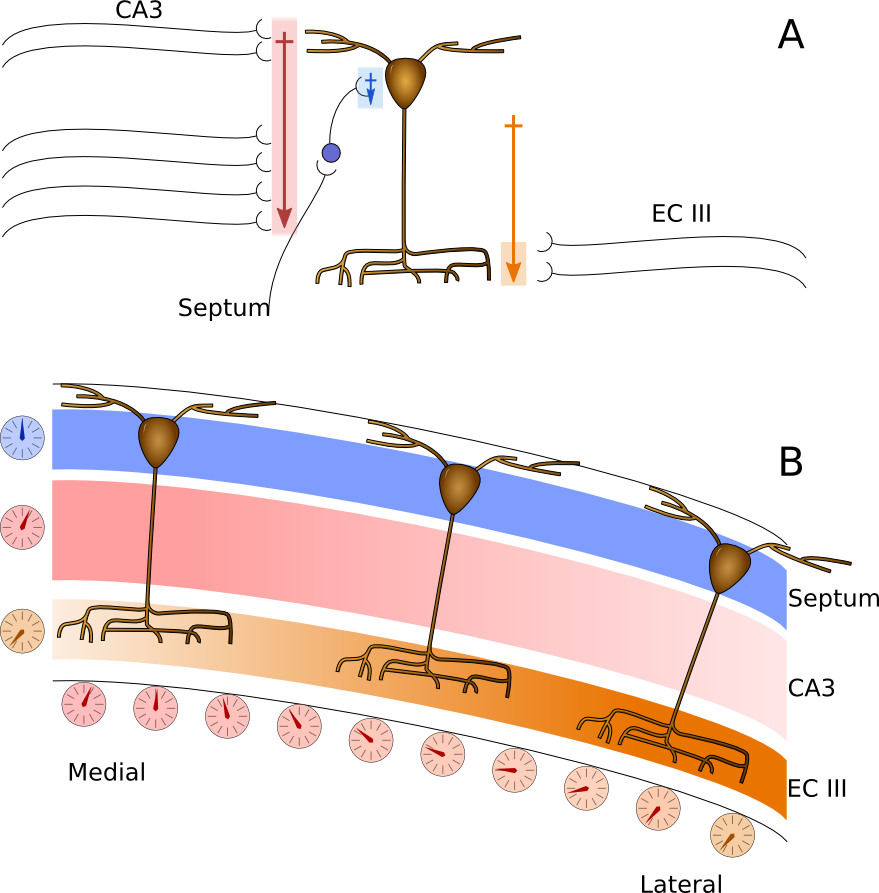
\includegraphics{./finalFigs/travelingwave/LFPModel.png}
\caption{\textbf{A model of spike timing and LFP driven by independent theta sources.}
\textbf{A.} Three major afferents contribute different types of
theta-modulated input to CA1 pyramidal cells. CA3 excitatory synapses
terminate primarily on the apical dendrite, but also on basal dendrites.
Entorhinal cortex layer 3 excitatory inputs terminate on distal apical
CA1 dendrites. The current path for these sources runs a long distance
from the synapse to the soma, causing large charge separation and long
dipoles easily detected in the local field potential. The magnitute of
the excitatory inputs determines the CA1 cell's spike rate. A third
theta rhythmic source comes from inhibitory synapses from local basket
and chandelier interneurons, which are in turn theta modulated by
GABAergic projection neurons in the medial septum. The inhibition causes
little change in membrane potential because it is due mainly to chloride
conductances, and therefore is not aparent in the field potential.
Instead it has a current-shunting effect and, in this model, modulates
the timing of CA1 spikes. B. Different theta sources exhibit different
phase profiles. Inhibitory currents are phase synchronized over the
extent of CA1. CA3 and entorhinal cortex may each exhibit traveling wave
patterns of anatomical phase offset, or they may each by internally
synchronized but at different phases from each other.}
\end{figure}

The distinction between different oscillatory factors could explain the
apparent paradox of synchronized theta sequences across CA1 cells with
desynchronized theta oscillations, even when spike times are
biophysically linked to theta. A model of this is illustrated in Figure
7. In the rate-to-phase model of Mehta and Wilson {[}37{]}, what exactly
is the inhibitory oscilation? It could be directly related to cortical
excitatory theta currents or septal inhibitory theta currents; the model
doesn't specify and there is not experimetal evidence to distinguish the
two. There may be phase offsets among excitatory currents but phase
synchrony among inhibitory currents. Septal inhibitory currents from a
single nucleus with gap junction coupling {[}61{]} may be synchronized
throughout hippocampus. If it is the inhibitory current that determines
the precise spike times of place cells, we would in fact expect theta
sequences to be anatomically synchronized.

Can we account for the effect of this model on the differing phase
relationships between inhibitory and excitatory theta currents in
different parts of the hippocampus? Excitatory cortical currents arise
from interactions between several inputs with various phases of their
own and relative projection strength that varies along the hippocampal
long axis. Since the excitatory currents come from different sources,
they are not mechanistically related to one another, and they may be in
phase at one location and out of phase at another. Can we account for
the related finding that the theta currents that drive spike timing are
synchronized when the local field potential and the bulk firing rates of
the cells are not? In modulating the spike rate, excitatory currents may
modulate bulk spike rate independently of the inhibitory current's
effect on spike timing, as it is excitation that drives a neuron's
membrane potential toward spiking in the first place. Likewise,
excitatory currents have a larger impact on the local field potential
because excitatory inputs terminate on distal regions of the apical
tree, and the flow of current through the synapse, down the detrite, and
out the soma, sets up long and spatial coherent extracellural dipoles.
Inhibitory currents by contrast are due to chloride conductances at the
soma, setting up very short dipoles and having only subtle effects on
the membrane voltage.

The excitatory input structures would not necssarily need to carry
traveling wave theta phase offsets. They may combine at CA1 in the same
mannar as described in Model 2, producing a phase gradient through a
single phase offset, and a gradient of relative connection strength.

This model retains the biophysical relationship between theta rhythms
and theta sequences in CA1 by attributing the inhibitory oscillation of
Mehta and Wilson's {[}37{]} excitation-to-phase model to anatomically
synchronized inhibitory shunting currents, and the LFP currents to
dipoles generated by independent excitatory afferents. It also suggests
that the inhibitory basket cells contributing the inhibitory theta
currents should be synchronized along the medial-lateral axis. This
prediction could be tested by measuring the theta phase preferences of
the basket and chandelier interneurons responsible for inhibitory theta
currents {[}10{]}.

A consequenece of the differential impact of two upstream regions on CA1
activity in general at different phases of the theta oscillation,
different segments of a theta sequences may have different roles or
reflect different sorts of computation. One popular model for instance
considers activity in the entorhinal cortex to reflect current sensory
input and activity in CA3 to reflect either model-based extrapolations
into the future {[}14,45,46{]} or completion of neural activity patterns
from degraded input {[}47{]}.

\subsubsection{Information timing is decoupled from bulk firing rate for
globally coherent coding}

The main contribution of this paper is the finding that theta sequences
as we understand them are impressively highly synchronized (to within
less than 10 ms) across large expanses (3 mm) of the hippocampus, and
that this synchronization is achieved in a context of desynchronized
rhythmic firing. This finding raises questions about which of the above
explanatory models (or an entirely different model) is responsible for
establishing this synchronization. We of course also want to know
whether this rule is true of the remaining 7mm of CA1, the most remote
end of which is thought to express some emotional content in favor of
seemingly arbitrarily-chosen spatial locations {[}62{]}; and we would
like to know whether theta sequences in upstream areas are synchronized
with those of CA1, or lead it by one or two synaptic delays.

Theta sequences appear promising as a foundation for an account of how
the hippocampus encodes spatial, mnemonic, and sequential information.
But it is important to point out that our understanding of the theta
sequence as we describe it now is still tainted by a faulty definition.
We define theta sequences as the ordering of spikes from place cells in
terms of the relative positions of their \emph{peak firing rates}.

This is problematic. For example, how would our results differ if,
unbeknownst to us, some place cells encode where the animal \emph{will
be} in the near future rather than where the animal is now? There is
experimental evidence that this is in fact the case {[}63--65{]}, and
that failing to account for it degrades the quality of position decoding
{[}66{]}.

Let's assume for the sake of argument that theta sequences are
temporally aligned throughout the hippocampus, but different parts of
the hippocampus preferentially participate in different parts of the
theta sequence, with place cells in very lateral positions only firing
in regions of the theta sequences that are two meters from the rat's
current position. In this example, the place field of the rat would
appear to be directly on top of the rat (this is how place fields are
now defined), and two meters behind the part of the track that the place
field is actually representing. The theta sequence that we decode will
not extend two meters, because the definition we have used for place
field will incorrectly attribute representation of the rat's current
location to that lateral cell's spiking. Now, two-meter-long theta
sequences have never been observed. Is this because they don't exist, or
because we typically do not account for the possibility of prospective
coding when we use the linear tracks that are optimized for recording
large numbers of place cells? We don't know. It will be important and
informative to try to address the issue of prospective coding in future
studies of theta sequences.

The use of firing rate in the definition of theta sequences is
problematic for a more general reason than the possibility of
prospective coding, though. Any spike that contributes to a theta
sequence is a spike that will impact the shape of the place field's rate
code as we currently define it (naively, the number of spikes fired as a
function of the rat's current location). Implicit in the notion of a
theta sequence is a separation between what a place cell encodes (we
take this as the peak of the firing rate profile), and when the place
cell expresses this encoding (a theta sequence is the unfolding in time
of encoding of a sequence of locations on the track). Imagine for the
sake of argument that a cell primarily interested in position x on the
track participate most heavily in theta sequences that extend from
behind the animal to ahead. By construction we are only manipulating the
``when'' of encoding, but by the definition of the rate field, we can't
avoid an effect on the ``what''. How much of a distorting effect does
the coupling of theta sequence firing have on our estimation of theta
sequences? We don't know, because although it may be appealing to remove
the firing rate field from the definition of theta sequences (or vice
versa), it is unclear what to replace it with.

\section{Real time position decoding from populations of place cells}

\subsection{Abstract}

Observational descriptions of hippocampal spatial encoding are outpacing
our understanding of their underlying mechanisms and ties to behavior.
The traditional manipulation techniques can not adequately target the
richly choreographed spiking sequences increasingly recognized as an
essential feature of spatial encoding. Some disruption specificity can
be achieved by leveraging known statistical relationships between
information content and the recency of spatial experience, and such
experiments have provided the first evidence of a link between sequence
replay and learning. But this method stops short of being able to
distinguish among the diverse forms of spatial content known to be
expressed in a single recording session.

A method of decoding spatial information content in real-time is needed.
To do this, we are developing a multi-tetrode recording system focused
on streaming representations of the processing stages typically used for
offline spatial decoding: spike detection, neural source separation
(cluster-cutting), position tracking, tuning curve extraction, and
Bayesian stimulus reconstruction. We also extend a method for position
reconstruction without human spike-sorting to operate in real time. Our
implementation makes critical use of Haskell, a programming language
that aides software development by strictly separating a program's logic
from its effects on program state, greatly simplifying code and
eliminating large classes of common software bugs. We describe the
capabilities and limits of our recording system, its implementation, and
routes for contributors to add functionality; and we survey the classes
of questions that could benefit from real-time stimulus reconstruction
and feedback.

\subsection{Introduction}

\subsubsection{Theta sequences and replay in place cells, phenomenology}

Temporally compressed spike sequences are increasingly recognized as an
essential feature of hippocampal encoding of space. Each increase in our
ability to sample large numbers of cells in freely navigating rats has
been accompanied by further support this claim {[}67,68{]}.

Physiologists are aware of two forms of sequential encoding. The first
occurs during active navigation. The majority {[}69{]} of spiking
activity in the hippocampus is due to place cells {[}3{]}, which spike
only when the rat is within an approximately 1 meter span of the track
particular to that place cell (the cell's ``place field''). At any given
time, the rat is within the (partially overlapping) place fields of many
place cells. Rather than fire in random order, the spikes are arranged
in precise sequences, with spikes from cells with place fields centered
just behind the rat first, spikes from place fields centered ahead of
the rat last, and a continuum between {[}17{]}. This sequence reflects
the sequences of place field centers that the rat would encounter on the
track, except it is sped up eight times and repeated once per cycle of
the underlying 7-10 Hz ``theta'' oscillation in the local field
potential {[}18,19{]}.

A second form of sequenced spiking occurs while rats are paused on the
track, consuming rewards or grooming. At these times, the hippocampus
emits irregular, 100-500 ms bursts of local field potential ``sharp
wave-ripples''(SW-R's) and spiking activity, with spikes ordered in time
according to the spatial ordering of their respective place fields
{[}54,70{]}. These are known as 'sequence replay' events. Sequence
replay often represents a track other than the track that the rat is
currently running on {[}71{]}; indeed it was first observed in sleeping
rats {[}72{]}.

\subsubsection{Summary of replay disruption studies}

In contrast to the large number of studies exploring the phenomenology
of theta sequences and sequence replay {[}20,21,71,73,74{]},
interventional studies are rare, because any specific activity pattern
of interest is embedded in a network also exhibiting off-target
sequences, and sequences themselves are not apparent to the experimenter
without extensive post-processing.

The content of sequence replay has a tendency to reflect recent
experience, however. Some investigators using SW-R's as a trigger for
immediate activity disruption have taken advantage of this to achieve
some degree of stimulus selectivity in replay disruption. Ego-Stengel
and Wilson {[}75{]} and Girardeau et. al. {[}76{]} used this paradigm to
show that selective disruption of sleep sequence replay of one track can
delay the acquisition of a spatial task on that track, relative to
another track. And Jadhav et. al. {[}77{]} disrupted all awake sequence
replay and showed that this impacts working memory performance.

Using real time decoding, we could refine these experiments by
disrupting only those replay events that correspond to the experimental
portion of the maze, and leave replay of the control portion intact.
This would provide more specificity in the question of whether relay is
required for consolidation during sleep an working-memory performance.

\subsubsection{Rationale for information-dependent replay manipulation}

We would like to ask much more specific questions of sequence replay
than whether or not it is needed for learning, of course {[}78{]}. Very
fundamental things are still not known about replay. For instance, is
its contents available to the animal for decision making? Are the
contents under the rat's volitional control (as imagination is under
humans' volitional control)? Definitive answers to these questions are
hard to come by, but we could restrict the space of possibilities. By
rewarding the rat for producing one type of replay and punishing him for
producing another, an increase in production of the former by the rat
would indicate that replay content is under the rat's control (although
the mechanism of control may be very indirect). A lack of ability to
adapt replay contents to the conditioning paradigm would suggest the
opposite. In a complementary experiment, the experimental selection of a
correct arm in a T maze could be determined by the rat's most recent
replay before the trial - left-going replay will cause left to be the
correct direction on the next trial, and vice versa. The ability to use
this information or not gives us some evidence about the question of
whether the rat is conscious of the content of his replay. Although in
this case too, the consciousness may be of something incidentally
correlated with replay content, rather than the content itself; so a
lack of ability to learn a replay-guided behavior may be more
informative than the positive result.

There are also some uses involving replay manipulation as more of a tool
than a scientific question. For instance, we might like to test the
hypothesis that replay events shape the properties of place cells on
subsequent laps. If we have a means of encouraging an animal to produce
large or small amounts of sequence replay for a given part of the track,
then we have some experimental control over replay as an independent
variable, and we can measure the subsequent effects of up-regulating or
down-regulating it on place field shape.

Leaving the realm of sequence replay (but still considering ensemble
stimulus reconstruction), these techniques could be useful for BMI
applications.

\subsubsection{Online replay decoding challenges}

Position decoding has been used for several years as a means of
summarizing the data of large numbers of place cells with multiple place
fields {[}21,55,71{]}, and thanks to Zhang's report {[}55{]} it is not a
difficult analysis to do. But porting it to the real time context, where
information is available in a streaming fashion instead of being
presented all at once, presents some interesting and surprising
challenges.

The first issue is \emph{throughput} - processing all of the data for
time \(x\) to \(x+\delta\) must happen in less than \(\delta\) time on
average, or else a backlog of unfinished work will completely swamp the
system. A related problem is \emph{latency} - even if the system has
sufficient \emph{throughput} to keep up with the data stream, each
computation step must finish with a small fixed offset from the time the
data was acquired, if it is going to be useful for the experiment. The
latency requirements for a behavioral feedback are generally lax, around
500ms, because we only need to detect a replay quickly enough to deliver
some form of reward to the rat. Other experiments have much tighter
latency requirements; interrupting an ongoing replay requires responses
closer to 50 ms from the actual replay event.

Next we have to consider the \emph{space complexity} and \emph{time
complexity} of the data structures and algorithms we choose {[}79{]}.
Different data structures have different advantages and disadvantages
that are typically ignored in offline analysis. A classic example of
this is the distinction between arrays and linked lists {[}80{]}. Arrays
can be indexed in constant time (the time needed to look up up the
n\textsuperscript{th} element does not depend on the size of the array)
but do not support adding new values. On the other hand, linked lists
allow appending elements in constant time, but indexing time is linearly
proportional to the index. Data structures vary in the amount of space
they take To cope with long-running experiments, we must avoid data
structures that grow linearly with the number of spikes processed.

Finally there is the practical concern that different inputs are coming
into the system at the same time, \emph{concurrently}. Offline, we can
ignore time and process the entirety of one electrode's signals at once,
then iterate over the rest - that is of course not possible in real time
ensemble-recording settings. In addition to the multiplicity of
tetrodes, we have data additional concurrent data sources from the
position tracking system and the input of the user. The process of
decoding the data is conceptually concurrent from the incorporation of
training data into the model. In general, concurrency and parallelism
are the source of a large number of subtle bugs, and thus there is a
great deal of active research into making concurrent computation more
robust {[}81--85{]}.

\subsubsection{Minimizing human intervention: no time for manual spike
sorting}

The most labor-intensive part of the post-processing involves sorting
the multi-unit spiking activity recorded on each tetrode into the
single-unit spike trains of putative single neurons. It is often
impractical to manually segment many tetrodes' spikes into putative
single units, especially during a real time experiment, when clusters
need to be cut before any real time feedback can be administered.

Kloosterman et. al. {[}86{]} developed a method for Bayesian stimulus
decoding from tetrode data without explicit spike sorting and provided
an implementation in MATLAB. This implementation is only suitable for
offline position due to the use of algorithms that take time
proportional to the number of processed spikes, and the poor performance
characteristics of MATLAB. But we can address these issues by
re-implementing the idea using different data structures and algorithms,
in a language with good concurrent programming support.

\subsubsection{A proof of concept in c and Haskell}

Here we report on two advances toward this goal. The first is a new
system for simple acquisition, band-pass filtering, and multi-unit spike
detection capable of running in tandem with our existing recording
systems. The second is a proof-of-concept application that streams raw
spike data and rat position data from the hard disk, performs source
separation based on previously-determined waveform discrimination
criteria, builds place field models, and performs the Bayesian inference
to reveal sequence encoding, all in real time.

The data acquisition system was written in a mix of c++ and Python,
where signal processing and networking can be done using common
libraries within grasp for beginners (which we were at the time). The
real time decoding system presented more interesting challenges, in
terms modeling place fields, supporting infinite data streams, and
concurrency. For this system, we turned to Haskell {[}87{]}, a language
optimized for ease of building composable abstractions {[}88{]}, through
the marriage of a highly extensible static type system and functional
purity. Haskell's type system enables the programmer to build custom
times that capture the much of the intent of a model or algorithm,
allowing the large classes of bugs to be eliminated by the compiler.
Functional purity is an engineering discipline strictly enforced by
Haskell that forbids variables from changing their values during program
execution. This restriction, thought apparently limiting, has many
highly favorable consequences for managing complexity. These features
fit together exceptionally well for designing highly concurrent
programs, a notoriously difficult task in all programming languages
{[}83,85{]}.

Our application currently reads spikes in multiple files at the rate
they were initially recorded, passes them through previously-determined
cluster boundaries, combines them with a record of the rat's position
also stored in a file, and produces a stream of place fields and a
composite visualization of the rat's position in real time. As we
develop the application, it will be able to interface with the system
performing the real time recording, track the rat in real time,
accommodate stimuli other than spatial location, and sort spikes into
single units without manual cluster-cutting.

\subsection{Materials and Methods}

\subsubsection{Backend signal acquisition and networking}

Raw data is acquired simultaneously, at 32kHz, from 32 channels
simultaneously on 2 NI PCI-6259 analog-to-digital converter cards
(National Instruments), using the NIDaqMX c API. After passing data from
the driver's memory to our program, samples are written into a circular
buffer and passed through a 4th order Butterworth IIR filter. This
choice of filter requires only two samples of history per channel,
imposing a very short delay (\textless{} 1ms) between the collection of
a given sample and subsequent processing. Spikes are detected by
comparing each sample to a threshold, noting threshold crossings, and
then waiting for one or a few cycles of acquisition until enough samples
have been collected to meet the waveform length required by the user.
Parameters like filter properties, spike threshold, and spike waveform
length are initially set in a configuration file, and later modified
through a networked API, so that the program can be run without an
immediate graphical user interface - this is a preferable arrangement
for a parallel, potentially distributed system, in which we may want a
single command issued by the user to affect recording systems running on
multiple computers.

Our previous recording system (AD., M.A.W.) also ran as a distributed
collection of low-end acquisition computers receiving analog signals as
input. In order to compare the recording quality and timing of our new
system to the old system, we physically split sets of four analog inputs
to two separate amplifiers - one serving each recording system. AD
relies on hardware filtering of broadband data into the spike waveform
band (300-6000 Hz) by a 3rd order Butterworth filter. ArtE reduces the
hardware system requirements by digitally filtering a single broadband
input into two signal bands - the spike band and the local field
potential band (0.1 - 475 Hz), in each case using a digital filter
designed to mirror the properties of AD's analog filters. Finally, using
both systems in tandem required careful time-base coordination. Using
standard computer system clocks is completely inadequate, as network
delays between computers are on the order of several milliseconds, and
can vary depending on system load. Instead, we route a digital clock
signal used to synchronize the AD computers into the ArtE system, and
manually issue a counter resetting command to ArtE over the network
while AD does the same for its own synchronization process. This fairly
hard-coded time-base integration is one problem that will have to be
solved before ArtE can be used in isolation from AD, but not a very
difficult one.

Isolated spike waveforms as well as down-sampled, continuous local field
potential signals are saved to disk in a different format from the one
used in the rest of our cluster-cutting and analysis workflow. Until
these tools are rewritten to work with the ArtE data format, we convert
ArtE files into AD format, and continue with xclust (M.A.W.) for
cluster-cutting and MATLAB (Mathworks, Natick MA) for general analysis.

\subsubsection{Offline position reconstruction}

We compute fast timescale summaries of neural ensemble activity through
Bayesian stimulus decoding, as described in Zhang et. al. {[}55{]}.
Implementations of this procedure to date, including those used in our
lab {[}21{]} are decidedly unfriendly to streaming, as they build models
of place fields by sorting all spikes from the beginning of the
recording session into the spatial bins partitioning the track. This
operation has time and space complexity linear in the number of recorded
spikes, making it unsuitable for continuous streaming. Place field
computations derived late in the recording would take longer than those
computed at the beginning, and memory would be exhausted in finite time.
These problems do not interfere with offline position decoding, because
place fields may be computed once,slowly, and used repeatedly. The
computation of many place fields that are synthesized into a single
position estimate may be computed serially.

\subsubsection{Online position reconstruction}

Modifying the place field models to update in constant time, rather than
performing a linear-time re-computation for each incoming spike, is
straightforward. Treatment of a large number of such models in parallel,
rather than serially, is more challenging, because these models are
ultimately combined into a single position estimate. Additionally, the
process of model update must run concurrently with graphic renderings,
user input, and the regular computation of the position estimate itself.

To perform Bayesian decoding in real time, we left the relative comfort
of c++ and MATLAB for Haskell, on the promise that Haskell's type system
and functional purity guarantees would simplify the static design of the
model, and aid in the highly concurrent data flow.

\subsubsection{Modeling place fields with Haskell data types}

The phenomenology of place fields and the diversity of maze environments
add complexity to the core notion of computing the place field, which is
simply spike rate as a function of track position. These complexities
are generally addressed in an ad-hoc way appropriate to each experiment.
Due to the increased engineering effort involved in performing
reconstruction in real time, we aimed to anticipate as many of these
issues as possible in the design of our stimulus model. We specify mazes
as a collection of spatial bins, each with a user-assigned ``outbound''
direction and physical width. An animal's relationship to the
environment is thus the combination of its relationship two each spatial
bin in three respects, (1) physical proximity to the bin, (2)
``outbound'' or ``inbound'' heading with respect to the bin, and (3)
position of the head with respect to the track width, either
``centered'' or ``leaning over''.

Matrix-based languages like MATLAB and c would suggest a representation
of a place field as a three-dimensional array (with bin identity in the
first dimension, the two possible heading directions in the second
dimension, and head-overhang in the third dimension, for example). A
particular position is referenced as an index into that array (for
instance, the value at field{[}14,1,2{]} could correspond to a stored
value related to the 14th spatial bin, inbound running direction, head
overhanging the edge). This is error prone. It requires the programmer
to remember the mapping between matrix dimension and stimulus dimension,
as well as a mapping between discreet values and stimulus levels (for
example, than 1 means ``inbound'' and 2 means ``outbound''). Naming the
levels with variables does not solve the problem, because the variable
``outboundLevel'' and ``headOverhanging'' are both of the same type.
Accidentally swapping the two (for example, writing
\(field[14, headOverhanging, outboundDir]\) ) will result in code that
compiles and runs, but produces incorrect output.

Haskell idioms are much safer. Instead of indexing into a matrix using
three Integers, an idiomatic Haskell solution would be to use a triple
of indices with different types as the addressable space over which
occupancy or a place field is defined. The use of distinct types for
bin, direction, and alignment 'indices' allows the compiler to check the
work of the programmer at every point where indexing happens. This small
difference in approach eliminates a very large fraction of the bugs a
codebase acquires as it changes and incorporates new features over time.
If the matrix dimensionality were to change to accommodate a new
feature, the Haskell compiler would enforce that this change is
accounted for at every point where the code tries to access the matrix.
This is in stark contrast to the flexible addressing of MATLAB and the
untyped addressing of c/c++ arrays - in both of these cases the change
may not result in any complaint from the program, but will instead
happily deliver either noisy (or worse, structured but incorrect) data.

Our Haskell model of the track is the basis for the model of the rat's
instantaneous ``position'', the model of accumulated time spend at each
position (the ``occupancy'' function), and the model of a place field.
At each point in time, we compute the animal's ``position'' as its
relationship to each bin. In the simplest case, the bin that the rat
occupies is given a score of 1.0, and all other bins scored 0.0; more
typically, we assign graded scores to the bins according to their
proximity to the rat; this method is favorable for smoothing noise in
place field computations. For those time bins when the animal is
running, this instantaneous position function added to an running tally
of time spent at each position (``occupancy'').

A place field is modeled in a similar manner to the occupancy map - as a
function from spatial bin to a number roughly equivalent to a ``spike
count'' in that bin. Each time a neuron fires a spike, the instantaneous
position map is added to the place field function accumulated so far. In
the simple case when the spatial bin containing the animal is assigned a
1.0, each spike adds an integer to that spatial bin in the place field.
When position is taken by the more usual Gaussian-smoothed method, each
spike adds a Gaussian curve to the accumulated field. This procedure
gives us constant-time, constant-memory spike-count functions that are
simple to update, while respecting the complexity of the underlying
behavior (the separate consideration for outbound vs. inbound running
direction, and the consideration of whether the head is aligned with the
track or leaning over the edge). When needed, the actual firing rate
function can be computed, in constant time, by dividing the neuron's
specific spike-rate function by the global occupancy function, at each
spatial bin.

\subsubsection{Managing concurrency and data streaming}

To decode in real time, we must simultaneously update place fields with
information from new spikes, update the current position of the rat,
read the place fields and combine them into a single position estimate,
handle user input, and render something to the screen. All of these
operations interact with the same underlying data, and thus the problem
is inherently in a difficult programming regime. Due to strict
enforcement of functional purity and immutable data, Haskell is in a
special position to simplify concurrent computations. Indeed, the STM
library provides a lockless concurrency scheme that allows multiple
threads to simultaneously modify the same data if they wish (this
generally leads to data corruption), as long as the only variables
modified are of a special type provisioned by the library, called TVars.
STM tracks access to these variables, detects when two threads have made
conflicting changes, and roles both changes back, allowing the threads
to attempt their modifications again.

We took advantage of the STM library to coordinate this concurrent read
and write access to a single state value. This value was stored in one
large TVar, which could be updated in the infrequent event of user input
or the addition of new tetrodes. Within the enclosing state value, each
place field is stored in its own TVar. In this scheme a very large
number of spikes can be distributed to their respective place fields,
and updates can be made without regard for the activity of other place
field updates.

The problem is not amenable to processing by entirely independent
threads (``embarrassingly parallel''), because the decoding step
requires access to all place fields. In addition to place field updates,
we accumulate spike-counts within short time windows, and the decoding
thread must reset all of these counts to zero each time a position
estimate is produced. We group the resetting of all place field cell
counts into a single atomic operation, to prevent the data
inconsistencies that would inevitably arise if count-updating and
count-resetting were interleaved. The grouping of actions into atomic
blocks that can be retried upon collision is precisely the strength of
the STM library that makes it so suitable for the structure of our
decoding algorithm.

\subsubsection{Clusterless decoding}

We extended the clusterless decoding method of Kloosterman et. al.
{[}86{]} by providing a new implementation that runs in bounded memory
and time (Kloosterman's takes time and memory proportional to the number
of spikes recorded, which makes it too slow for large-scale,
long-running recordings). To restructure the algorithm in a way that
would continue to perform with potentially-infinite streams of data, we
turned again to Haskell for its ease of use when working with custom
data structures.

Kloosterman et. al.'s algorithm requires the comparison of
recently-received spikes (the testing-set) to the amplitudes of all
spikes received from the beginning of recording (the training-set) along
with the rat's track location during those training-set spikes. An
estimate of the rat's position at testing-time is derived through
Bayesian inference over a combination of the training-set spikes
weighted by their amplitude-similarity to the testing-set spikes. A
literal implementation of this algorithm has the disadvantage of making
a larger and larger number of comparisons as the experiment progresses
and the training-set grows. An obvious alternative would be to divide
the space of spike amplitudes into a set of cubes, and update the cube
into which each training-spike falls with the rat's current position.
However, because amplitude space is four dimensional, the number of
cubes required to tile amplitude space at a reasonable resolution is too
large to store in computer memory. Sparse matrices and KD-trees are two
good data structures for holding multi-dimensional data in limited
memory. We chose the re-implement clusterless decoding using the latter,
at a slight performance penalty, because trees are somewhat more
convenient to work with than matrices in Haskell. In order to
accommodate new training-set spikes in bounded memory, when a new spike
arrives less than some threshold distance from its nearest neighbor, the
two are combined into one, and the payloads of the two (the place
fields) are summed according to each point's weight.

\subsection{Results}

The results of our effort to date are a working real time decoding
algorithm and a proof-of-concept system of supporting infrastructure.
The core algorithm takes advantage of Haskell's highly efficient runtime
system and composable concurrency model to combine spiking and
positional information in real time and produce a streaming Bayesian
estimate of the rat's location. The bandwidth of the system is
sufficient for decoding fast-timescale features like theta sequences and
sequence replay. The development process itself made critical use of
Haskell's type system features, which drastically improve the
programmer's ability to reorganize code and discover logical and
typographical errors at the time of program compilation.

\subsubsection{Decoding fast-timescale features: theta sequences and
replay}

Simply decoding the rat's position is a potentially useful engineering
goal, but in general the rat's instantaneous position is more
conveniently estimated using an overhead camera. The features we are
really interested in gaining real time access to are those internal
states that deviate from the rat's physical location; and these
deviations happen on a very fast timescale - the timescale of theta
sequences and sequence replay. Thus one of our primary design goals was
to achieve a processing bandwidth capable of estimating the rat's
position in 20ms time windows. Figure 8 shows a position estimate
computed post-hoc (top row), and the estimate derived from real time
processing of the same data, at a lower spatial resolution (bottom row).
The data set used included 33 place cells recorded on 8 tetrodes. This
is combination of spatial resolution and cell count was near the
processing limit for our machine, although we expect that the bandwidth
will increase substantially when the various cell-sorting tasks are
split among multiple computers, as they would be in a full recording
system. The middle and right panels show decoded theta sequences and
sequence replay respectively.

\begin{figure}[htbp]
\centering
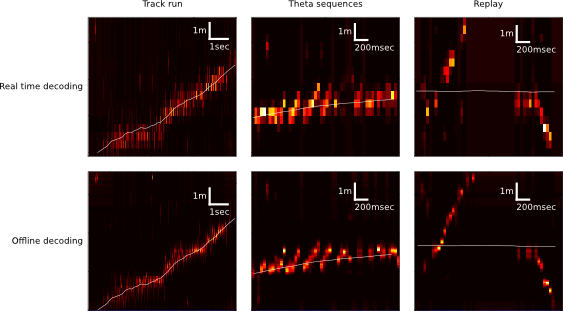
\includegraphics{./finalFigs/headToHeadDecoding.png}
\caption{\textbf{Fast time-scale position decoding.} Reconstructed
features computed in real time by the ArtE decoder (bottom row) match
those derived post-hoc (top row). The features are harder to resolve in
the ArtE case because we decoding position at a courser spatial scale
(20 cm bins \emph{vs.} 3.5 cm bins), but are still sufficient for the
detection of events that would be used as triggers in a closed-loop
experiment. Theta sequences (middle) and sequence replay (right) are
both recoverable from a typical place cell population in real time.}
\end{figure}

\subsubsection{Decoding speed and real time requirements}

One drawback of using STM to manage concurrency is that performance can
be more than we would like. Measurements of individual processing stages
do not give much actionable information about contention over shared
memory. We ran the ArtE position decoder and recorded the timing of its
outputs in two conditions - on a laptop with 4 cores before the
diagnosis of a slow memory leak, and on a faster desktop machine with 8
cores after the removal of the leak. In the poor-performance case, half
way through the session, the system ceases to be able to keep up with
the stream of incoming data and enters into an oscillation between
seconds-long chokes and purges. In the better-performing case, decoding
continued reliably over the duration of the recording session, tending
to produce a position estimate once every 20 ms, with occasional
\textless{} 100 ms excursions.

\begin{figure}[htbp]
\centering
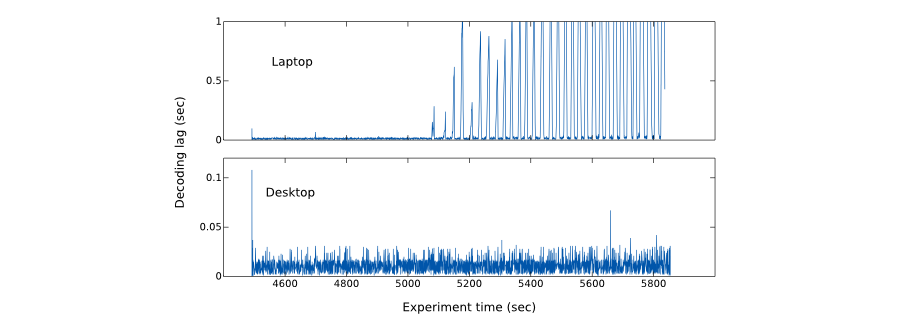
\includegraphics{./finalFigs/arteTiming.png}
\caption{\textbf{A timing failure mode.} Running a version of the ArtE
decoder with a slow space leak on a laptop results in the eventual
inability for the system to keep up with incoming data, and a series of
long interruptions in the decoding. Removing the source of the memory
leak and running on a fast desktop, fast responses remained for the
duration of the recording session, with occasionally lags of several
tens of milliseconds.}
\end{figure}

\subsubsection{Bugs, deadlocks, crashes and performance debugging}

As promised by the Haskell marketing material, bugs in the Haskell code
that passed compilation were very rare, and bugs that did not pass
compilation were generally very easy to find.\footnote{They were
  underlined by in red within emacs, thanks to the integration between
  emacs and the GHC compiler provided by ghc-mod (Kazu Yamamoto)}
Subjectively speaking, runtime crashes and deadlocks were exceedingly
rare\footnote{A scientific study of the occurrence of various types of
  bugs in code written by practitioners of various languages in a
  scientific setting would be very interesting.} The bugs that do remain
tend to involve improperly specified algorithms (things like sign-flips
or reassembling the wrong pieces when mixing the contents of two data
structures and the pieces have identical types), and performance bugs,
which can occur due to the improper handling of Haskell's lazy semantics
and the accidental buildup of large collections of unevaluated function
applications.

When performance bugs become apparent in a program's runtime behavior,
they can often be tracked down by time and memory profiling. The
following is trace of the memory usage of the decoder, broken down by
code module. We see that a module we have no control over (System) is
using the most memory, but that the usage is constant. On the other
hand, our own Histogram module has a memory footprint that is growing
linearly with time over the five-minute trace interval. This is sure to
cause problems down the road as the runtime system continuously manages
a growing pile of unused memory. In this case, we simply removed the
Histogram (it was an extraneous visualization widget) to check that it
was the source of our performance bug. We can fix it using a
finer-grained version of the same approach, breaking memory usage down
by function rather than module.

\begin{figure}[htbp]
\centering
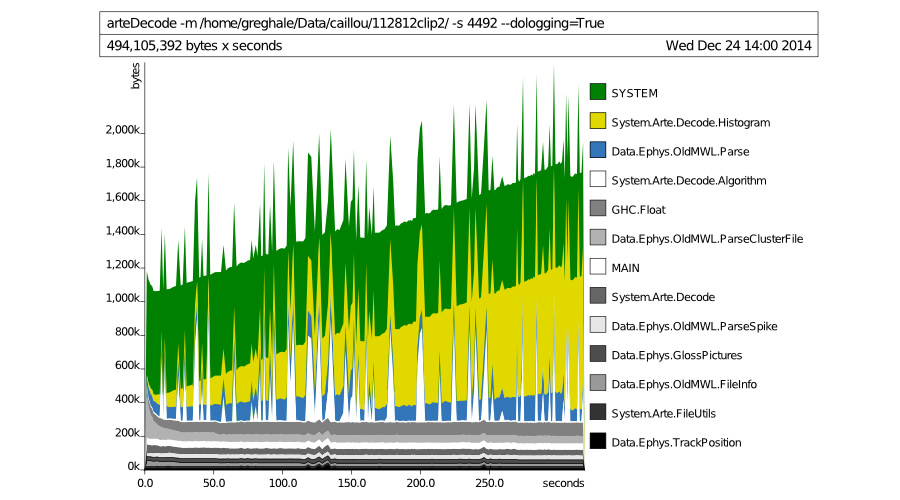
\includegraphics{./finalFigs/arteDecodeProfile.png}
\caption{\textbf{Memory profiling helps performance debugging.} Most
Haskell debugging is performance debugging, because it can be hard to
see which parts of a program will accumulate resources over time. The
GHC Haskell compiler produced this plot of memory usage over time broken
down by module. The runtime system uses the most memory (green). The
Histogram module (yellow), which is part of the ArtE project, fails to
release data and grows linearly with time. These profiles generally make
it easy to find the code errors that lead to ramping memory use and
program slowdowns.}
\end{figure}

\subsection{Discussion}

\subsubsection{A tool for decoding streaming place cell data}

We have developed a working algorithm and a proof-of-concept test system
for performing Bayesian stimulus decoding {[}21,55{]} on populations of
place cells in real time. The implementation makes critical use of
Haskell's type system, extensive open source libraries {[}87{]}, fast
runtime {[}89--91{]}, and concurrency and parallelism support
{[}92--94{]} (specifically, using the GHC Haskell compiler {[}87{]}).

As other users of Haskell have noted, one difficulty in writing fast
code is avoiding patterns that interact poorly with Haskell's lazy
evaluation semantics {[}95{]}. This was a stumbling block in our
implementation as well, as some mistakes lead to slowdowns that become
evident only after several minutes of running, and are therefore
difficult to eliminate by trial and error. Fortunately the GHC compiler
provides tools for tracking memory and time usage; these tools greatly
aided our performance debugging experience.

\subsubsection{Remaining components needed to run experiments}

Several components need to be built before our decoding system can be
used in closed-loop experiments:

\begin{itemize}
\itemsep1pt\parskip0pt\parsep0pt
\item
  \emph{Tracker}: Rat tracking software capable of linearizing twisted
  tracks and transforming 3D position into 1D track location and heading
  direction.
\item
  \emph{Replay discriminator}: A means of deciding from the stream of
  decoded positions, when a pattern counts as \emph{replay}. This must
  be customizable enough to fit different experimental demands, such as
  conditioning feedback on a replay's virtual run direction on a T-maze.
\item
  \emph{Networked decoding}: A means of splitting the work of model
  training and model testing across multiple computers, to remove the
  CPU decoding bottleneck and allow the use of more than eight tetrodes
\item
  \emph{Network transport}: A common protocol for packaging various
  types of data (animal location, neuron spikes, intermediate decoding
  data, behavioral sensor values, maze actuator commands, etc). Ad-hoc
  networking is not quite sufficient because many of our components need
  to fan out to multiple listeners (e.g. a spike source) or fan in from
  many sources (e.g. the stimulus decoder).
\end{itemize}

We plan to develop these components ourselves in same way that we
developed the ArtE backend system, by replacing one component at a time
into the existing AD recording system built by Matthew Wilson and Loren
Frank, and doing integration tests comparing AD's native output to the
output with one adapted component. Although there is a lot of work left
to do before the system can do end-to-end work, it's not too early to
start fantasizing about the experimental possibilities. We describe some
of these in the next section.

\subsubsection{Possible experiments using real time decoding}

An important set of experiments to do is to refine the ripple disruption
studies {[}75--77{]}. The goal of these studies was to determine whether
or not sequence replay is necessary for memory consolidation (in the
case of {[}75,76{]}) or working memory (in the case of {[}77{]}). Jadhav
et. al. disrupted all ripple-related activity on the track. There was no
attempt made to restrict ripple disruption to the ripples carrying one
type of replay or another\footnote{In fact, their control condition was
  to begin inhibition 200ms after ripple detection, with the intention
  of finding a disruption scheme with similar timing characteristics to
  ripples and avoiding times when the animal is running, without
  blocking ripples themselves. As Davidson et. al. {[}21{]} and Layton
  and Wilson {[}96{]} showed, some replay events are longer than 200 ms,
  and if these were present in the Jadhav study, they may have been
  truncated.}. They found that this disruption interferes with the rat's
ability to choose a maze turn direction based on recent memory, but does
not interfere with maze choices that have only long-term memory
requirements. But they could not tell, for example, whether individual
replay events carry the short-term memory trace used by the rats on
individual trials, or whether replay disruption is generally upsetting
to performance of the more difficult phase of the task. Indeed, task
difficulty is a factor that often distinguishes between the experimental
and control phases of a behavioral task{[}97{]}, but it is not often
acknowledged as one. With online replay content detection, the two
equally difficult working-memory tasks of the Jadhav study could have
been made controls for one another, by selectively disrupting replay
corresponding to one of them.

Ego-Stengel and Wilson {[}75{]} and Gerardeau et. al. {[}76{]} used the
fact that replay of recently experienced tracks is more common during
sleep than replay of tracks learned several days ago in order to
selectively disrupt the replay of one track over another. In
experimental designs like these, having the ability to single out one
type of replay for disruption would further refine the selectivity,
perhaps enhancing the differential effects on behavior.

Real time replay detection provides opportunities for experimental
designs that weren't possible before. Fewer than half of replay events
during wake contain decodable spatial content pertaining to the current
maze {[}21{]}, and the fraction in sleep is much smaller {[}72,98{]}. If
we want to make reward or task contingency conditional on replay, then
decoding replay content in real time is a hard requirement.

For example, we may want to test whether left-going replay on a
T-maze\footnote{Alternatively, some behavioral factor correlated with
  replay!} can be used as the behavioral response that is rewarded or
punished to produce operant conditioning, in a specific way that doesn't
generalize to right-going replay, to test whether the content of replay
or a behavioral correlate of that content is something cognitively
available to the rat.

There is currently very little evidence for a one-to-one connection
between replay content and immediate past or present behavior
{[}21,73,99{]}. The dual of the operant conditioning experiment would be
to try to train a rat to recognize that, whichever direction his most
recent replay took, that is the direction he must run next to find a
reward.

A third class of experiments is nebulous but probably very valuable.
Using real time Bayesian position decoding (not necessarily replay
detection per-se), an experimenter would have immediate access to the
joint activity of the recorded population of place cells. Many classical
discoveries in neuroscience are due to chance observations rather than
premeditated binary-choice hypothesis-based predictions. The discover of
place cells themselves {[}3{]} is due to tinkering with a rat while
listening to the audio amplified spiking of an individual hippocampal
neuron; as was the discovery of the primary visual cortex simple
receptive field {[}100{]} and the large literature that
followed\footnote{Oriented moving bars of light were famously discovered
  to be the optimal stimulus for driving spiking in the cells of primary
  visual cortex when David Hubel and Torsten Wiesel were changing slides
  in a projector slide deck; although the many pictures of animals and
  natural stimuli on the slides failed to elicit a response, the
  sweeping motion of the edge of the slide as slides were being changed
  in and out of the machine caused very robust spiking. Hubel and Wiesel
  creatively pointed their projector at a chalk board, systematically
  moving the slide edge and making chalk marks at the edge locations and
  orientations that best excited the cell nearest the electrode. This
  approach is what we mean by using real time feedback for 'tinkering'.}
We expect that when decoded position is available to the experimenter,
creativity in the moment will lead to informal experimentation that
sheds light on the nature of replay in a way that would not be possible
with the traditional, slow data collection / data analysis cycle.

\section{Retrosplenial slow-wave wake and interaction with hippocampus}

\subsection{Abstract}

Cortical slow waves interact with the hippocampus during sleep, in the
timing of their oscillations and the information content of local neural
ensembles. These interactions are thought to be involved in memory
consolidation. Here we show that slow-wave like activity in the
retrosplenial cortex is not confined to periods of behavioral sleep, but
also accompanies hippocampal ripples and replay during awake reward
consumption. During initial exposure to a maze, many hippocampal
transitions into the offline state are accompanied by slow-wave sleep
features. Later in learning, slow-wave sleep like activity is less
prevalent during the consumption of small rewards, but can reliably be
elicited with large rewards. This activity is similarly prevalent during
both light and dark phases of the sleep cycle, suggesting that in is not
a function of drowsiness. We propose that the offline state of the
hippocampus is not a time of hippocampal isolation from all cortex.
Rather, the same mnemonic processing thought to rely on
cortico-hippocampal interaction may also occur during wake.

\subsection{Introduction}

\subsubsection{Cortico-hippocampal sleep interactions, possible role in
memory}

Both cortex and hippocampus exhibit interesting forms of structured
activity in sleeping animals. In the hippocampus, a brain rhythm known
as a sharp-wave ripple is known to carry information about sequences of
locations on a recently visited track {[}21,54,70,72{]}. The
information-richness of these coordinated activity patterns makes us
hopeful that there are inroads into understanding the encoding of
information and its mechanism of storage. It is thought that cortex has
a role in long term information storage, and that sleep is as an
important time for memory formation {[}101--104{]}. The interactions
between hippocampal activity and cortical activity may provide clues
about the role of sequence replay in the rest of the brain, the
mechanism of information transfer from hippocampus to cortex, and the
mechanisms of that information's long-term storage.

\subsubsection{Slow wave oscillations cleanly distinguish between
sleeping and awake cortex}

The most striking feature of cortical activity in the sleeping brain is
a pattern known as \emph{up-down states}, the \emph{delta rhythm}, or
\emph{frames}, depending on the recording method.\footnote{\emph{Up-down
  states} refers to intracellular recordings, \emph{Delta oscillations}
  to EEG + LFP, and \emph{frames} to extracellular multi-unit recording
  respectively. We use the term frames where the distinction is not
  important} They are three views of the same underlying phenomenon: the
coordinated switching between an online, wake-like state with spikes,
and a hyperpolarized state profoundly devoid of spikes.

This pattern is not seen while an animal is awake. It has so far only
been observed in animals that are drowsey{[}105{]} or in slow-wave
sleep{[}106{]}, one of the two primary sleep stages. The other sleep
stage, REM sleep.\footnote{REM stands for \emph{Rapid eye movement}. REM
  sleep is accompanied by movements of the eyes that resemble awake
  visual exploration {[}107,108{]}.} REM sleep is also referred to as
\emph{paradoxical sleep}, because of the similarity of REM brain
activity to activity patterns in awake animals.

\subsubsection{Theta and ripples distinguish between 'online' and
'offline' hippocampus}

The hippocampus is similar to cortex in that it has two very different
modes of operation, but they are not as strictly linked to sleep and
wake as the activity patterns in cortex are. Instead, they reflect the
'online' or 'offline' nature of attention. During visual exploration,
running, foraging, etc. (and during REM sleep) the hippocampus and many
of its input and output structures are engaged in an 7-10 Hz oscillation
called the \emph{theta rhythm} {[}9{]}. When an animal's attention is
directed inward and while the animal is in slow-wave sleep, theta ceases
and is replaced by \emph{Large irregular activity}, a generally quiet
state interrupted by \textasciitilde{}50ms bouts of coordinated vigorous
spiking{[}109{]}, sometimes grouped into \emph{ripple bursts} that last
half a second {[}96{]}.

\subsubsection{Retrosplenial cortex unexpectedly follows HPC into
SWS-like state during reward}

One popular model proposes that memory formation goes in two stages:
while animals are awake, sensory information flows through the cortex
and into the hippocampus, where it is assembled into short-lived mental
models of the various sorts of things to be remembered; and while they
are sleeping the hippocampus projects a modeled form of this information
back to the cortex, with repetition, for long-term storage {[}110{]}.
This model serves as a backdrop for designing experiments that examine
the effect that concrete hippocampal events have on cortex, and that
concrete cortical events have on hippocampus.

\subsection{Materials \& Methods}

\subsubsection{Subjects}

All procedures were approved by the Committee on Animal Care at
Massachusetts Institute of Technology and followed US National
Institutes of Health guidelines. Tetrode arrays were assembled and
implanted according to the procedure in Nguyen et. at. {[}52{]} and
Kloosterman et. al. {[}53{]}. We made several modifications to the
materials and procedures to improve our multi-cell sampling. First, we
glued several hundred half-inch pieces of 29 gauge and 30 gauge
hypodermic tubing into rows about 6 mm long, then stacked and glued the
rows together to form a honeycomb patterned jig, for organizing the
tetrode guide-tubes that would eventually inhabit the microdrive.
Second, we developed the ArtE recording system (detailed in Chapter 2)
to run in parallel with our usual usual tetrode recording rig. The
broader goals of the ArtE project are to enable real-time data analysis
and feedback, but in this experiment we used it merely to increase the
number of simultaneously recorded tetrodes.

\subsubsection{Single-unit tetrode recording}

We constructed a tetrode guide jig by cluing together several hundred 2
cm strips of 30-gauge polyimide tubing
(\href{Ihttp://www.minvasivecomponents.com}{IW MinVasive Components})
into a dense 'honeycomb' pattern, one tube at a time. Starting with a
single row of 30 tubes, and then building upwards, each new tube was
secured to the honeycomb with medium thickness cyanoacrylate glue
(\href{http://www.greatplanes.com/accys/gpmr6001.html}{GreatPlanes}).
This is a tedious process. The result is an array of hexagonally-spaced
30-gauge tubes. From these several hundred, we selected 32 tubes that
would become the target sites for individual tetrodes, with several
targeting hippocampal CA1, several targeting retrosplenial cortex, and
several targeting anterior dorsal thalamus (these thalamic tetrodes are
not analyzed in this study). We inserted 10 cm stainless steel wires (5
milliinch diameter) partially into the selected tubes, and on the
exposed ends, we loaded 32 10 cm lengths of 30 gauge polyimide tube.
These 32 tubes were glued together in place with Teets dental acrylic,
and the bundle was removed as a unit, and integrated into a tetrode
hyperdrive according to the instructions at Jove {[}52,53{]}.

Craniotomy templates were printed on paper with a standard laser-jet
printer, with markings corresponding to the guide tube bundles. Marks
were printed for bregma and lambda skull points too. Plastic
transparency sheet was placed on top of this diagram and holes were cut
to accommodate the drive bundles; needle holes were made at the bregma
and lambda points. We sterilized this plastic cutout and used it during
surgery at a stencil, using sterilized pencil to mark the locations of
the craniotomy. This ensures that the craniotomy will perfectly fit the
peculiar shape of the tetrode guide tubes.

Tetrodes were lowered into the pyramidal cell layer of CA1 over the
course of 2 to 3 weeks and left there for several more weeks of
recording. We sought to maximize the number of neurons recorded and to
minimize within-experiment drift, so we closely tracked the shape of
sharp wave ripples (which undergo characteristic changes during approach
to the cell layer) and later the amplitudes of emerging clusters. If
either of these factors changed overnight to a greater degree than
expected, the tetrode was retracted by 30 to 60 micrometers.

\subsubsection{Behavioral training}

Behavioral training consisted of rewarding rats for simply running back
and forth on a curved 3.4 meter linear track, or running continuously
clockwise on a 3.4 meter long circular track, with rewards given for
every 360 degrees of running for the first 3 laps and for every 270
degrees thereafter. Food deprivation began one or two days prior to the
beginning of acquisition, with rats receiving 30 grams of food per day,
adjusted up or down depending on the rat's motivation to run and level
of comfort (assessed by the amount sleep taken before the running
session). The target food-deprived weight was 80\% of free-feeding
weight, but we rarely achieved this without disrupting the sleep of the
animals, so body weights tended to be 90\% of the free-feeding weight or
more, especially after rats learned the simple rules of the task.
Additionally, we occasionally provided large rewards throughout training
(2-3 grams of wetted powdered rat chow), to encourage the long stopping
periods during which awake replay can be observed. Most rewards we
delivered were 200-300 milligrams. Under these conditions, rats run for
about 20 laps or 30 minutes before becoming satiated and ignoring
rewards. In some cases, rats continued to express interest in track
running, but we aborted the trial early because continuous running in a
single direction causes coiling of the electrical tether and torsion on
the head.

\subsubsection{Electrophysiological Characterization}

Spikes and local field potentials were voltage buffered and recorded
against a common white-matter reference, at 32 kHz and 2kHz
respectively, and the rat's position was tracked at 15 Hz through a pair
of alternating LED's mounted on the headstage, as in Davidson et. al.
{[}21{]}. Spikes were clustered manually using the custom program,
xclust3 (M.A.W.). Place fields were computed for each neuron as in Zhang
et. al. {[}55{]}, by partitioning the track into 50 to 100 spatial bins,
and dividing the number of spikes occurring with the rat in each spatial
bin by the amount of time spent in that spatial bin, in each case only
counting events when the rat was moving at least 10 cm/second around the
track. Direction of running was also taken into account, allowing us to
compute separate tuning curves for the two directions of running, which
we label 'outbound' and 'inbound'.

\subsubsection{Frame detection}

The multi-unit spikes with peak-to-trough with width greater 0.4
milliseconds from each tetrode were counted in non-overlapping 1 ms
windows to compute firing rate. Down-states were defined as
interruptions in cortical electrode spiking activity lasting at least 10
seconds with an average (over tetrode) spike rate of at most 40 Hz.
Candidate down-states that were interrupted for less than 5 milliseconds
were merged into one. Up-states (or ``frames") were defined as any time
in between dips greater than 10 milliseconds and less than 3 seconds in
length.

\subsection{Results}

\subsubsection{Characterizing slow-wave sleep (SWS) in cortex}

Slow-wave sleep is dominated by large irregular activity in the
hippocampus, which consists of periods of desynchronized activity,
interrupted by sporadic \textasciitilde{}50ms bursts of activity from
large numbers of cells. These bursts are associated with about 50ms-long
monophasic or biphasic spikes in the local field potential, bouts of
\textasciitilde{}200 Hz rhythmic activity called ripples, and large
amounts of multi-unit spiking activity (Figure 11 top, sharp-wave
ripples marked in blue).

During this time, retrosplenial cortex is engaged in the slow
oscillations of slow-wave sleep, with spiking activity collected into
up-states lasting 250ms to two seconds, with intervening 10 to 100ms
down-states (Figure 11 green arrows) that coincide with either spindles,
K-complexes or delta rhythm cycles, depending on the depth of slow wave
sleep (Figure 11 bottom).

\begin{figure}[htbp]
\centering
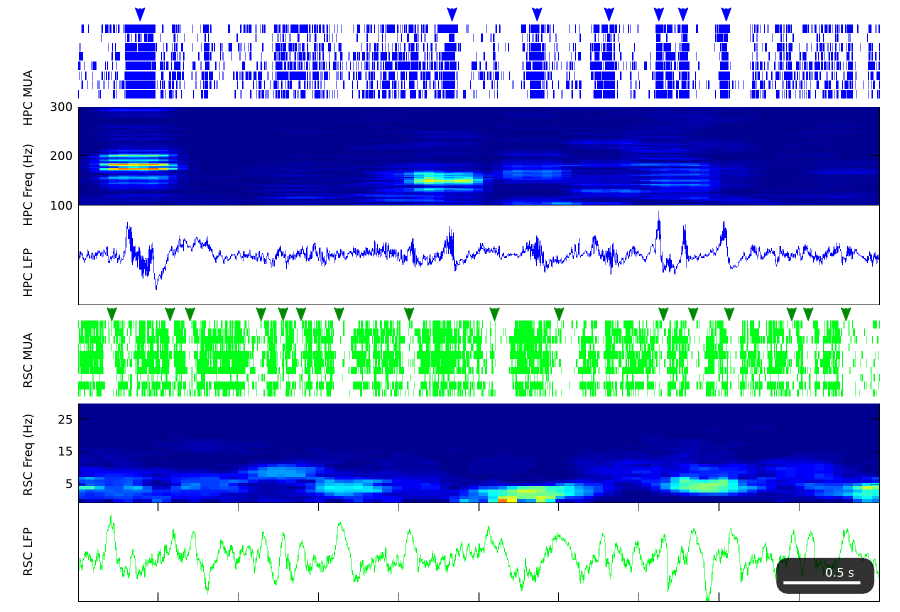
\includegraphics{./finalFigs/SWW/exampleSleep.png}
\caption{\textbf{Slow-wave sleep features in retrosplenial cortex and
hippocampus.} \emph{Top:} Five seconds of multi-unit activity, LFP
spectrogram, and LFP raw trace from the hippocampus during slow-wave
sleep. Blue arrows mark sharp-wave ripples. \emph{Bottom:} Multi-unit
activity, LFP spectrogram, and LFP raw trace of retrosplenial cortex
during the same period. Green arrows mark down states, interruptions in
the ongoing cortical spiking.}
\end{figure}

\subsubsection{Retrosplenial cortex enters SWS-like state during novelty
/ large rewards}

We trained rats to run clockwise around a 3.4 meter circumference track
to receive food reward (Figure 12), in order to engage navigational
circuits in the hippocampus as well as head-direction circuits in
retrosplenial cortex. Most rewards were a small 200-300mg bolus of
wetted powdered rat chow, delivered at a single point on the track
(requiring a full lap for delivery) for three laps. On subsequent laps,
we rewarded the rat once for each 270° degrees of track running (for
reasons not related to this study - we were reusing the task design of a
study we were aiming to replicate about REM replay {[}111{]}). Once in
every 4 to 6 trials, we instead used a 3g bolus, to encourage the rat to
stop, eat, and produce more ripples and replay events from the
hippocampus. In later phases of the experiment, we moved a number of
electrodes up from hippocampus into somatosensory and motor areas, to
explore further the phenomenon we noticed in retrosplenial cortex.
During track running and sleep, we often listened to the amplified
activity of either hippocampus or cortex (switching the audio monitor
back and forth over the course of 30 minute sessions).

\begin{figure}[htbp]
\centering
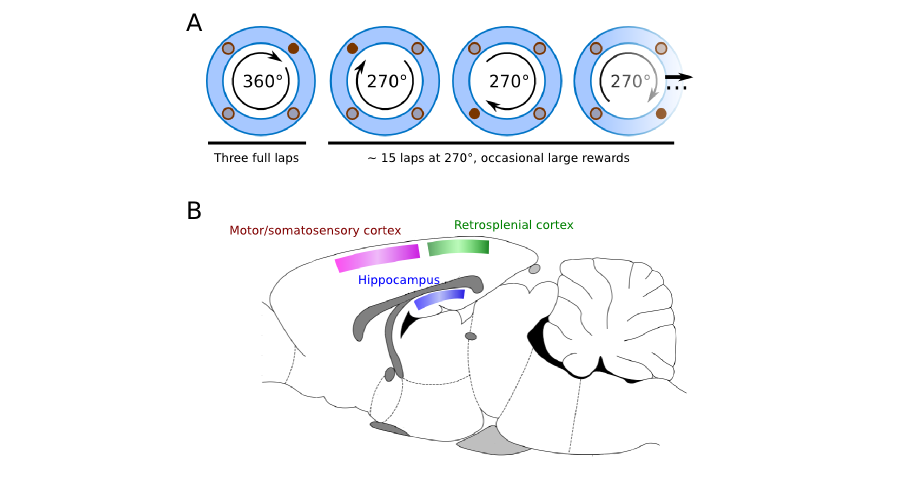
\includegraphics{./finalFigs/SWW/expDesign.png}
\caption{\textbf{Recording sites and behavioral training.} \emph{Top:}
Behavioral training was carried out every day over the course of the
recording and consisted of clockwise running on a 3.4 meter circular
track. For the first the rat got normal (200-300 mg) rewards. For the
remainder of the session (usually 10 to 20 laps) normal reward was
delivered every 270°, but occasional normal rewards were replaced with
large (2-3 g) rewards, to encourage longer pauses and more hippocampal
replay.}
\end{figure}

We became accustomed to the sound of ripples and spindles in the
multi-unit spiking activity of cortex in the sleeping rat. We were
surprised to hear a subjectively similar pattern from retrosplenial
cortex while rats stopped to eat large rewards. Comparing the raster
plots and LFPs of several, retrosplenial cortex activity transiently but
strongly resembles the structure of activity during slow-wave sleep
(Figure 13), with characteristic sharp breaks in ongoing activity and
accompanying K-complex like LFP oscillations. In another set of
experiments, conducted at the end of a 5-hour period of sustained wake
in the middle of the day, we recorded activity during foraging in an
open field, using novel objects to keep the rat in a curious state and
preventing him from sleeping on the maze. During these periods of
drowsiness, we saw similar interruptions in ongoing retrosplenial cortex
spiking.

\begin{figure}[htbp]
\centering
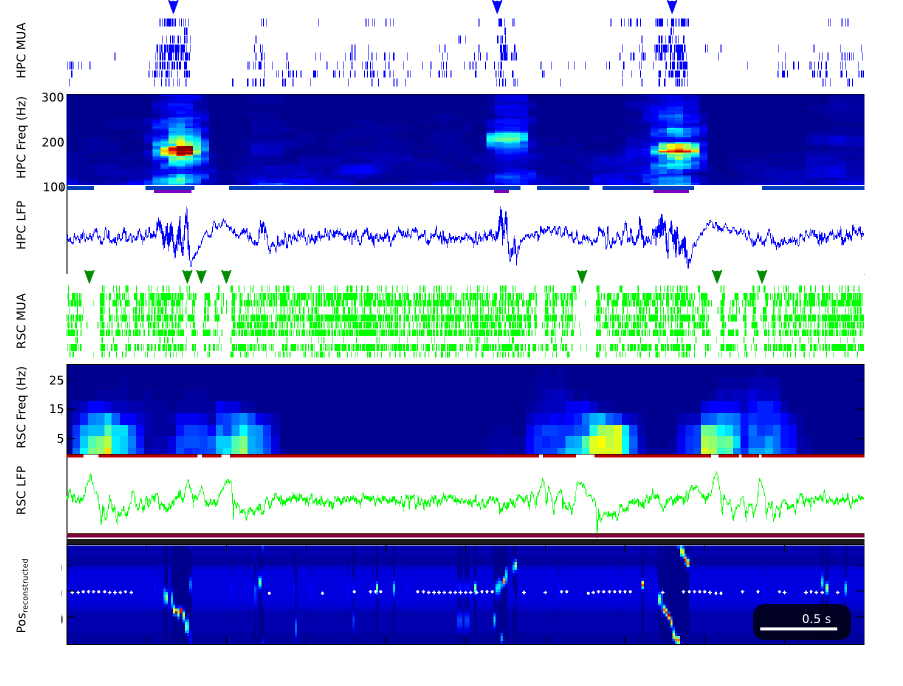
\includegraphics{./finalFigs/SWW/exampleDetail.png}
\caption{\textbf{Slow-wave sleep like features in awake retrosplenial
cortex.} Five seconds of activity in hippocampus and retrosplenial
cortex during the consumption of large reward on the track. \emph{Top:}
Multi-unit activity, LFP spectrogram and LFP trace from the hippocampus,
with sharp-wave ripples indicated by blue arrows. \emph{Bottom:}
Multi-unit activity, LFP spectrogram, and LFP trace from a
representative tetrode in the retrosplenial cortex over the same
interval. Crossings below the spike rate threshold used for frame
detection indicated by green arrows. Note the similarity to the
slow-wave pattern in slow-wave sleep shown in Figure 11. \emph{Far
bottom:} Position trace (white dots) and reconstructed position from
hippocampal place cells. Awake sequence replay events co-occur with some
hippocampal ripple bursts.}
\end{figure}

Examining longer periods of time, we can find that the epochs dominated
by hippocampal large irregular activity, ripples and replay events are
the same epochs dominated by slow-wave sleep-like activity in
retrosplenial cortex. Figure 13 shows a 60 second pause on the track,
the first half of which exhibits slow-wave sleep-like features, and the
second half of which does not. Although the rat is not making forward
progress on the track during the second half of the pause, hippocampus
and retrosplenial cortex are both in `online' mode, so presumably the
rat is still but attentive.

\begin{figure}[htbp]
\centering
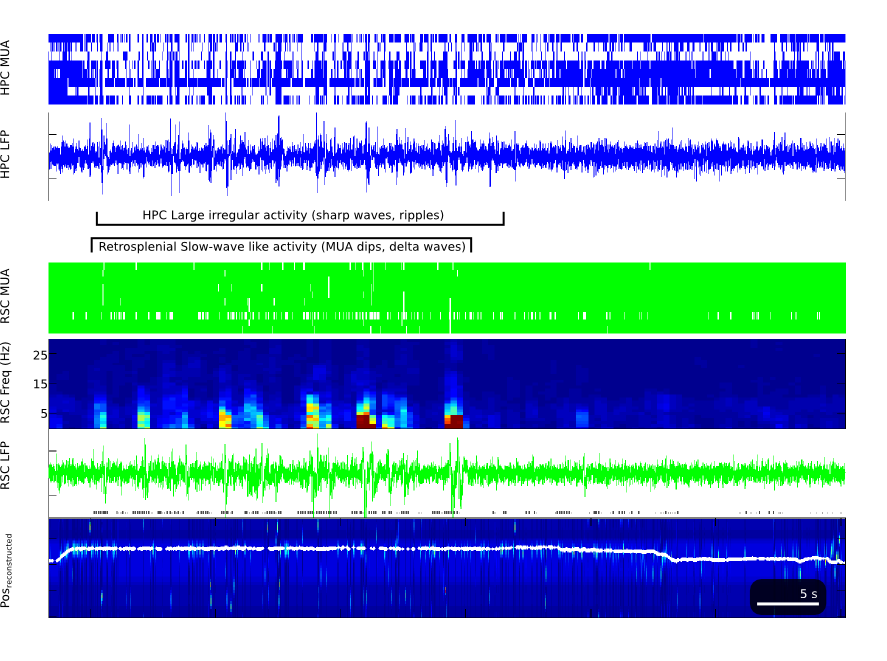
\includegraphics{./finalFigs/SWW/exampleExtended.png}
\caption{\textbf{Retrosplenial slow-wave sleep and hippocampal awake
large irregular activity occupy the same behavioral epochs.} A sixty
second sample of activity in hippocampus and retrosplenial cortex during
the consumption of large reward on the track. \emph{Top:} Multi-unit
activity and an LFP trace from the hippocampus. For the first half of
the stopping period, hippocampus is in an offline state with occasional
bursts of ripples. \emph{Bottom:} Multi-unit activity, LFP spectrogram,
and LFP trace from a representative tetrode in the retrosplenial cortex
over the same 60 second interval. The first half of the stopping period
is marked by a sporadic K-complexes and down-state-like interruptions of
the ongoing spiking. \emph{Far bottom:} Position trace (white dots) and
reconstructed position from hippocampal place cells.}
\end{figure}

\subsubsection{RSC awake slow waves coordinate with hippocampus under
diverse conditions}

To determine whether slow-wave like activity is related to familiarity
or drowsiness, we recorded it early and late in behavioral training, and
during both the light and dark phases of the light cycle. Early in
training, both ripples and frames appear in response to large and small
rewards (Figure 15, top). Later in training, ripples may still appear
during the collection of small rewards, but down-states are more
restricted to large reward consumption (Figure 15, bottom). To determine
whether slow-wave sleep like activity is related to drowsiness, we
attempted to eliminate it by providing a rat two day's rest and then
running him during the dark phase of the light cycle, when rats are more
active (Figure 15, middle). We continued to see very strong slow-wave
like activity during these sessions.

\begin{figure}[htbp]
\centering
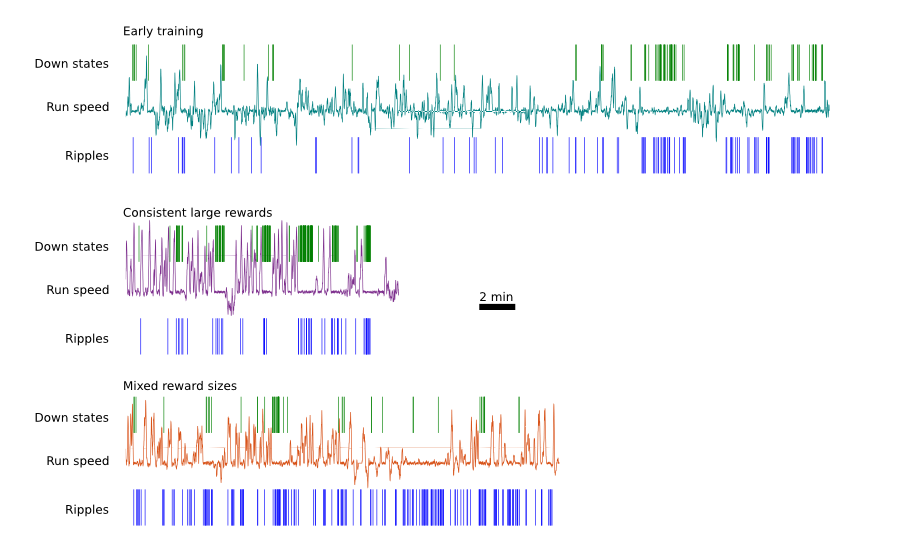
\includegraphics{./finalFigs/SWW/manyLongExamples.png}
\caption{\textbf{Behavioral scale alignment between slow-wave like
activity and hippocampal ripples, during two phases of the light cycle
and early in training.} Retrosplenial slow-wave like activity can arise
under diverse conditions, but is always associated with a hippocampal
offline state. Down states detected as sharp drops in cortical firing
rate are indicated as green raster tics over the course of three
training sessions. Ripples detected by increases in hippocampal firing
rate and ripple-frequency LFP power are indicated in blue. \emph{Top:}
Early in training down states occur during both short and long pauses on
the track. \emph{Middle:} A recording session taken in the middle of the
wake phase of the light cycle late in training. Ripples and down states
largely avoid short stopping periods and small rewards. \emph{Bottom:} A
typical recording session late in training, during the light phase of
the light cycle. Down states are largely restricted to long eating
pauses; ripples are more prevalent during long pauses but also present
during collection of small rewards.}
\end{figure}

\subsubsection{Anatomical restriction - non-participation in other
cortical areas}

In later recording sessions, we retracted most of the hippocampal
tetrodes up into overlying somatosensory and motor cortices and recorded
from these in tandem with the retrosplenial cortex. We saw clear
slow-wave modulation of these tetrodes during slow-wave sleep and a
degree of participation during drowsiness. However no spontaneous down
states, frames, or K-complexes were seen during wake.

\begin{figure}[htbp]
\centering
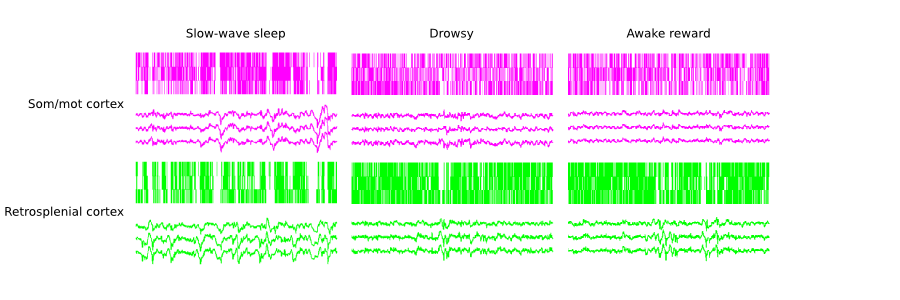
\includegraphics{./finalFigs/SWW/finding.png}
\caption{\textbf{Example frames in SWS, drowsiness, and large reward consumption.}
Example frames and down states are clearly visible and coordinated
between retrosplenial cortex (green) and somatosensory and motor
cortices (magenta) during SWS. Down states are less frequent during
drowsiness and reward consumption. In drowsiness, weak coordination
between cortical areas can be seen. During awake reward consumption,
frames and down states are visible in retrosplenial cortex, but
somatosensory and motor cortex fire as they normally do during wake.}
\end{figure}

In the retrosplenial cortex, lengths of putative down states in
slow-wave sleep, drowsiness, and consumption of large reward were
distributed similarly (Figure 17). The same is true of the scattered
somatosensory and motor cortex electrodes, with the exception that thees
only exhibited down-states during slow-wave sleep and drowsiness. We
found no down states meeting our criterion of 5 milliseconds at less
than 40 Hz multiunit activity in somatosensory and motor cortex
tetrodes.

\begin{figure}[htbp]
\centering

\includegraphics{./finalFigs/SWW/downStateLengthDistributions.png}
\caption{\textbf{Distribution of down-state lengths in SWS, drowsiness,
and large reward consumption.} Down states were defined as intervals
with mean spike rate per tetrode below 40 Hz lasting for at least least
5 ms. Down states in retrosplenial cortex and somatosensory cortex are
similarly distributed. The distribution appears during large reward
consemption periods in retrosplenial cortex, while no awake down states
were seen in somatosensory and motor cortex.}
\end{figure}

\subsection{Discussion}

\subsubsection{Awake slow-waves in RSC, coordinated with HPC, fully
awake}

We show that in retrosplenial cortex, slow-wave sleep like activity can
be reliably elicited in the fully awake rat using large rewards. This
activity could be elicited in fully-awake rats and drowsy rats. Early in
behavioral training, it occasionally occurred during the consumption of
small rewards. Late in training it occurred preferentially in response
to large rewards.

Furthermore, this activity is coordinated on the behavioral timescale
with the \emph{offline-mode} of activity in hippocampus, which is
already known to engage in large irregular activity {[}109{]} during
track pauses and reward consumption. The novel finding here is that the
hippocampus is not alone in this pattern.

\subsubsection{Comparison with Vyazovskiy's local sleep}

These results are similar to the \emph{local sleep} findings of
Vyazovskiy et. al. {[}105{]}, but the primary difference is that the
results we report seem to be unrelated to drowsiness, while Vyazovskiy's
\emph{local sleep} is strongly related to sleep need and momentary
behavioral impairment. Our findings suggest something else - that local
sleep may be a normal part of the waking state, and that the
hippocampal-cortical dialog previously thought to occur only during
sleep may also occur when large rewards are found.

To summarize, we think that Vyazovskiy et. al. are seeing the same thing
that we are seeing - slow waves. However, Vyazovskiy shows that the slow
waves of sleep can encroach on local cortical circuits at the times near
sleep. We show that slow waves may also appear in retrosplenial cortex
in a way that's otherwise unrelated to sleep.

\subsubsection{Functional roles for HPC-Cortex coordination may apply to
wake}

Very little is known about the effect of ripples and replay on ongoing
cortical activity. The finding that retrosplenial cortex follows the
same general activity pattern in wake gives us the opportunity to extend
work in hippocampal-cortical interactions during sleep to waking
periods.

Awake hippocampal-cortical interaction may share features with the
cortico-hippocampal interactions of sleep, such as the appearance of
up-down states in hippocampal interneurons {[}112{]} or the coordination
of encoded spatial content {[}98{]}.

\subsubsection{New questions raised by awake slow waves}

These findings raise a number of interesting questions. First, what
other brain areas coordinate with hippocampus during wake? Is this
phenomenon specific to retrosplenial cortex, or could be a feature of
all navigational cortical structures in the Papez circuit {[}113{]}? Or
is it a feature of the default mode network {[}114{]}? The retrosplenial
cortex is a member of both.

Then there is the question of mechanism. Slow wave sleep is thought to
arise from an interaction between cortex, relay thalamus, and inhibitory
reticular thalamus. In the case of retrosplenial cortex, the excitatory
thalamic afferent comes from the anterior dorsal thalamic nucleus (ADT).
This raises the obvious question, does anterior does ADT participate in
awake slow waves? Is there enough specificity in the connections from
ADT to the reticular nucleus such that slow waves could be expressed in
retrosplenial cortex without spilling over into other thalamo-cortical
loops? Or does more of the thalamus than ADT participate in awake slow
waves, and it is the cortex that suppresses these effects in order to
maintain the normal cortical activity while retrosplenial cortex adopts
sleep-like activity. All of these questions can be answered simply by
multi-site recording in a maze with large rewards, and this should
greatly expand our understanding of the role and extend of slow-wave
activity.

In addition to the parallels that may be drawn between functional roles
for sleep interactions and wake interactions, awake interactions may be
have some of their own unique features. The rest of the cortex is
behaving so dissimilarly between wake and slow-wave sleep that the
inputs to retrosplenial cortex between wake and sleep will be very
different. It is not necessarily the case that slow waves preclude the
processing of sensory information however. Rasch et. al. {[}115{]}
showed that the slow-wave sleep presentation of odors that were
previously paired with awake learning improve performance on the next
day.

\section{Conclusion / Wrap-up}

Our ultimate goal is to understand how information is encoded in the
brain, and how that encoding lends itself to permanent storage. Work on
place cells in the hippocampus is indicating that timing, populations,
and structured interactions among large numbers of neurons will be a key
part of the story of how information encoding and storage are achieved.
In answering some particular hypothesis-driven questions, it may be
enough to collect a few cells each from a large number of animals. But
to go beyond testing the hypotheses that our current paradigm can
generate, to discover new paradigms that involve the emergent phenomena
of numerous brain structures integrating rich streams of environmental
information with even richer mental models generated over a lifetime and
accessed at the whim of the organism, we will need to record from very
large numbers of neurons in many brain areas in naturalistic contexts
with great temporal precision.

The history of the tetrode recordings of the hippocampus in freely
moving animals provide evidence for this claim. Place cells and V1
orientation tuned cells were discovered using auditory feedback and a
very open-ended experimental paradigm. Online sequence replay was
discovered by taking an unbiased look at the simultaneous activity of
many place cells in an animal given the freedom to relax naturally
between laps on the track. In the realm of information coding,
information transmission, and memory, the parts of the brain under study
are complex enough that there is a great deal to be gained by optimizing
an experiment for open-ended interpretation. The key features of an
open-ended design are naturalistic conditions, very large populations of
data, high temporal resolution, and the ability for the experimenter to
access that data in real time for tinkering.

We have shown in this thesis that information encoding is precisely
timed in a global fashion within hippocampal CA1. The subsequent finding
that hippocampus and retrosplenial cortex interact during sequence
replay opens a window for moving beyond the co-occurrence of LFP events,
toward an understanding of how hippocampal information is moved to the
cortex and what form it takes while in the cortex. And our work on the
ArtE real time decoding system will hopefully give us a way to take
population-wide information encoding and render it into a form useful
for human experimenters in real time.

\section{Appendix A: Hippocampal anatomy and physiology background}

A brief reveiw of cellular organization in the hippocampus is given to
help the reader stay oriented during discussions of electrode placement
and traveling wave propagation. We also describe the freely moving rat's
local field potential signatures and single-unit spiking properties,
which are central to the rest of the thesis.

\subsection{Hippocampal anatomy: cell layer and dendritic layers}

The rat hippocampus is a curved, complex, three-dimensional structure
most easily thought of as a sheet {[}116{]}, about 10 by 7 mm face-on
and 1mm thick, folded into a 'C' shape first along its short axis, and
again into a larger 'C' along its long axis. The face of the sheet is
fully tiled by primarily excitatory pyramidal neurons. Their cell bodies
of these neurons are collected into a thin (about 0.1mm) band within the
sheet's 1mm thickness.

Basal dendritic arbors extending upward from the cell bodies toward the
skull (the hippocampus is inverted relative to cortex) for 0.25mm form
the \emph{stratum oriens}. Apical dendrites extend downward for 0.5mm
forming the \emph{stratum radiatum}, and then branch widely to form the
\emph{stratum laconosum moleculare}.

After folding and curling, the far end along the longer dimension of the
sheet terminates near the septal nuclei, and the other travels backward
and bends down to embed itself in temporal cortex. The long axis of the
hippocampus is referred to as the \emph{septo-temporal} axis.

The first folding of the sheet described above divides the
\emph{proximal-distal axis} into two parts, named CA3 and CA1 by Lorente
de Nó {[}117{]}, (CA stands for "cornu ammonis", or ram's horn, which is
reminiscent of the shape of the hippocampus in cross section).

CA3 dendrites receive most of their synaptic input from the
\emph{dentate gyrus}, entorhinal cortex, and the axons of other CA3
neurons. {[}116,118{]}. CA1 receives most of its input from CA3 and
entorhinal cortex, but does not project to itself {[}116{]}. These
patterns of inputs are more restricted than in many other parts of the
cortex and have lead to computational models that take advantage of a
layer with recurrent connections (CA3) connecting to one without (CA1),
but none have wide acceptance. We will see later that our understanding
of information processing within a single layer is incomplete, and this
makes it difficult to speculate on the nature information transmission
between areas.

\subsection{Hippocampal place cells}

Pyramidal cells increase their firing rate dramatically when rats enter
a particular part of a maze, as originally described by O'Keefe {[}3{]}.
The region of space eliciting spikes is that cell's \emph{place field}.
Typical place fields are roughly 20 and 80 centimeters long, and
different neurons have different place fields; recording about 30
neurons is enough to find a 3 meter track without any gaps in place
field coverage. Spiking rates outside of a neuron's place field are
quite low - often less than 0.1 Hz, and in-field rates peak rates are
reliable across trials, typically 10-30 Hz.

The behavior of place fields in response to rotations and distortions of
the maze is the subject of a large body of work, which can be summarized
in terms of map displacement, \emph{rate remapping} and \emph{global
remapping} {[}119{]}. \emph{Rate remapping} refers to a change in place
field peak firing rate and \emph{global remapping} a displacement in
place field location not necessarily in agreement with the displacements
experienced at the same time by other place cells. The rules governing
which sort of remapping will result from which types of maze
manipulation are complex and not completely consistent between studies,
to the point that the neurons themselves disagree on the rules in
particular instances and may fall at the same time in different
directions {[}120,121{]}. But in general, minor changes to the
appearance of the maze tend to elicit rate remapping {[}119,122{]} while
radical ones scramble the locations of place fields and produce global
remapping {[}122,123{]}.

A similar rule of thumb applies to most maze and cue displacement
results: place fields tend to follow what we would expect of a rat's
top-level model of where he is. Minor enlargements of the maze produce
proportional stretching and displacement of the place fields {[}124{]}.
A rotation of enough maze cues such that North is falsely recognized as
the old West will produce the appropriate rotation of place fields with
respect to the poles of the earth (and a lack of displacement with
respect to the cues){[}125{]}.

\subsection{Theta oscillations and multiunit spike phase}

Electrodes in the hippocampus pick up a 7-10 Hz, large-amplitude rhythm,
in addition to somatic spikes. This is called the \emph{theta rhythm}
{[}9,10{]}. The theta rhythm is present when animals are running or in a
stationary, attentive state, and during REM sleep {[}9{]}. Theta
oscillations can be found throughout CA1 and CA1, as well as in the
dentate gyrus and entorhinal context, and a host of other cortical and
subcortical areas. Collectively the areas expressing theta are known as
the \emph{Papez circuit} {[}113{]}. Incidentally a lesion to any
component of the Papez circuit produces in humans strong anterograde
amnesia (as reported in the hippocampal patient H.M. {[}126{]}, thought
in fact HM's entorhinal cortex was far more damaged than his hippocampus
{[}8{]}).

The mechanisms of theta's expression is being explored on two levels:
the level of the generation of rhythms in the neurons, and the level of
the translation of neural rhythms to extracellular currents {[}10{]}.
Neither level is completely understood, despite a large number of
studies lesioning or pharmacologically silencing specifically excitatory
or inhibitory neurons in various brain regions.

What is known is that two sources of theta can be pharmacologically
distinguished by atropine and NMDA antagonists {[}59,127{]}, and these
two components are associated with different intrinsic frequencies and
different behavioral states. \emph{Type 1} theta is insensitive to
systemically delivered atropine {[}127{]}. Its intrinsic frequency is
about 10 Hz and it is naturally elicited by running. \emph{Type 2} theta
is sensitive to atropine and is naturally elicited by stationary
attention. The importance of the septum in theta generation is strongly
suggested by the fact that lesions to it nearly eliminate the appearance
of theta in the local field potential throughout the rest of the brain.
But this is not the whole story, as a dissected hippocampus in a dish
will spontaneously express theta after application of acetylene
{[}128{]}. Interestingly, if that same hippocampus is pharmacologically
divided in two along its long axis by application of the GABA agonist
muscimol, then the two halves will oscillate at theta frequencies
differing by up to 1.3 Hz, with septal hippocampus being the faster
oscillator of the two. {[}128{]}.

Quite a few facts are also known about the connection between the
theta-rhythmic excitation of neurons and neuropil, and the appearance of
theta to an electrode in the form of a local field potential. These
details are important and interesting because of a connection between
the phase of the oscillation and the activities of place cells (which we
will discuss soon), and the phase of such an oscillation is such a
finicky thing. For one, applying different filters to the recorded
signal is enough to significantly advance or delay theta's apparent
phase {[}129{]}. For another, an electrode's view of the rhythm is
determined by the dipole environment local to it, and different parts of
a neuron's dendritic tree express different dipoles at different phases
of theta; so that the perceived phase of theta changes by half a cycle
as an electrode is moved through the thickness of the hippocampus.

Buzsaki in particular has done a lot of mapping of the electrical
sources of theta, first by lowering a single electrode in consistent
intervals {[}130{]} through the apical-basal axis and measuring
representative oscillations, and later by using probes with large
numbers of evenly spaced contacts {[}59{]}, and applying the
current-source-density technique, which predicts the spatial sinks and
sources of current within the tissue. To summarize these findings, the
\emph{Type 1} theta currents come mostly from pyramidal cell apical
dendrites near the hippocampal fissure and basal dendrites in stratum
oriens, while \emph{Type 2} currents are strongest in stratum radiatum
and are due to dentate and CA3 input. These two sources do not agree in
phase, and the effects of each drop off with distance of the recording
electrode from the source. This is why electrodes with different
placement will report different theta phases - they are respectively
closer to different theta sources {[}131{]}. The combined effects of the
multiple sources is still fairly sinusoidal, as the sources are fairly
sinusoidal and equal in frequency, and sine waves of equal frequency but
different phase generally sum to a sine wave of a new phase {[}132{]}.

\section{Appendix B: Sleep states and hippocampal-cortical interactions}

\subsection{Sleep stages, cortical EEG correlates (spindles, delta,
theta)}

Waking and sleep behavioral states are accompanied by very different
patterns of neural activity in the cortex and hippocampus. These
differences can be more pronounced that the modulations of firing rate
associated with encoding sensory information and producing particular
motor output. Some are easily detected through the human skull via EEG.
They are immediately apparent in the firing patterns of populations of
neurons and in the character of local field potentials recorded inside
the brain. We study these differences in order to understand the
function and mechanistic origins of sleep, as well as to gain clues
about how sensory stimuli are processed during waking and shut out
during sleep. We would also like to know whether the particular
signature activity patterns of sleep have functional roles themselves,
or in combination with other sleep-specific events in other brain areas.

Sleep in most animals {[}133{]} is divided into two categories
{[}134{]}: slow-wave sleep, named after the EEG oscillation associated
with it {[}106{]}; and REM sleep, named for the associated rapid
movement of the eyes {[}107{]}. The latter is also called ``paradoxical
sleep"\footnote{Perhaps if most sleep were REM sleep, then our
  nomenclature would be different, and what is now known as slow-wave
  sleep would have been called ``paradoxical activity", because sleep
  itself would no longer be the major discriminator between types of
  brain activity.}, because brain activity during REM sleep so closely
resembles brain activity in waking animals and because a relative small
fraction of mammalian sleep in REM sleep {[}135{]}.

Slow-wave sleep in humans can be further divided into four stages that
correspond to four levels of depth of sleep and are marked by different
combinations of signature EEG events{[}134{]}. Stage I sleep is
drowsiness and it is marked by the appearance of spindles, short bouts
of \textasciitilde{}10Hz oscillations lasting about a second each and
occurring from once a minute to ten times a minute until drowsiness
transitions into the next sleep stage. In stage II spindles become less
frequent and are replaced by occasional K-complexes, large, one-cycle
oscillations. Stage III and Stage IV sleep are both deep sleep; they
lack spindles altogether, and K-complexes have become part of a 1-4 Hz
``delta oscillation" {[}136{]}, the characteristic rhythm that gives
slow-wave sleep its name. Stages III and IV are differentiated by the
regularity of the slow waves (they are not very periodic, by the
standards of most waves) - in Stage III single cycles will vary in
length from 200 ms to 2 s.

\subsection{Up-down states in vitro, frames of cortical spikes during
sleep in vivo}

Delta oscillations of slow-wave sleep have a clear neural basis, the
synchronized spontaneous oscillations of cortical neurons {[}137{]}. The
extracellular peaks of the slow oscillation correspond to periods of
profound hyperpolarization and the complete absence of cortical spiking.
Intracellular voltage traces make the non-periodic nature of the slow
oscillation more clear; rather than a harmonic oscillation, there is a
clear bimodality in the distribution of membrane voltages:
\textasciitilde{}100ms blocks of -80mV without spiking interspersed
between blocks of -60mV with spiking. There is a large body of work on
the mechanisms of generation of this state; it is thought to involve
interaction with the thalamus (and in particular, inhibitory long-range
neurons of the thalamic reticular nucleus), which also profoundly
changes its mode of firing during sleep {[}138{]}.

\subsection{Hippocampal ripples and sleep replay, wake replay}

Activity in the hippocampus during awake active behavior is dominated by
the 10 Hz theta oscillation, which impacts the spiking of all neurons in
the hippocampus and is plainly visible in local field potential
recording and audible in the multi-unit spiking {[}9,139{]}. The
hippocampus of a rat in slow-wave sleep is very different. It is known
as ``large irregular activity"{[}109{]}, and it consists of quiet
periods interrupted by sporadic, vigorous bursts of spikes. The
collective activity of the neurons causes a \textasciitilde{}200 Hz
oscillation known as a ``ripple", which is usually accompanied by a
single cycle of a slower (\textasciitilde{}10 Hz) ``sharp wave". These
bursts of activity tend to last about 50 ms {[}140{]}, and often come in
pairs or triplets {[}96{]} of ripples in quick succession (a ``ripple
burst").

Unlike the cortex, however, sleep is not the primary determinant of
which mode of activity the hippocampus will be in. Large irregular
activity occurs in the hippocampus whenever an animal stops to groom,
consumes reward, or reaches the end of copulation {[}141{]}. Paradoxical
sleep in the hippocampus is marked by a sustained theta rhythm and the
absence of large irregular activity {[}9{]}.

\subsection{Hippocampal-cortical coordination}

Several recent studies have begun to show a link between the sleep
characteristics of cortex and those of hippocampus. Although the
hippocampus does not exhibit delta-frequency slow waves in its local
field potential, up-down states mirroring those in cortex are also
present in the membrane potential of hippocampal interneurons and the
granule cells of the hippocampal input structure, dentate gyrus
{[}112{]}. And the membrane potentials of some hippocampal CA3 and CA1
pyramidal cells are modulated at the times of cortical transitions from
down state to up state {[}142{]}.

The hippocampal ripples have also been found to coordinate in time with
cortical down-to-up state transitions {[}143{]} and cortical spindles
{[}144,145{]}, suggesting that these oscillatory events may be either a
reflection of information transfer between cortex and hippocampus, or
that they may be a mechanism by which that information is transferred.

The possibility of cortico-hippocampal information transfer became much
more concrete after the report by Ji and Wilson {[}ji2006coordinated{]}
that hippocampus and cortex express coordinated information content
during slow-wave sleep. Surprisingly, single neurons in primary visual
cortex (V1) fire spikes at specific locations on a maze, when that maze
is instrumented with visual cues on its floor (1 bit per spike in V1,
\emph{vs.} 3 bits per spike in hippocampus); and during sleep, the
sequence of V1 cells activated by the track spontaneously co-fire in the
same order during slow wave sleep, as place cells have been shown to do
in slow-wave sleep {[}72{]}. When both hippocampus and cortex re-express
in sleep a sequence learned in wake (admittedly a rare event, at least
with our current recording capabilities), they almost always agree on
\emph{what} sequence to replay {[}98{]}.

\section{Appendix C: Haskell}

\subsection{What is functional programming}

Functional programming is both a style of programming and a set of
language features designed to make functional programs natural to write
and performant. That style revolves around two novel notions of what a
function is. First, functions in a functional programming language are
analogous to functions in math - relationships between inputs in a
domain and return values in a range; they are guaranteed to return the
same result from the same inputs. Second, functions are themselves
'normal values' - they can be passed as arguments to other functions, or
returned from other functions as return values.

Languages like c allow a programmer to use functions in this way but do
not make it easy. C is modeled closely on computer hardware, a context
that emphasizes allocating memory and manipulating it. These operations
are not 'functional' in the mathematical sense, because they involve
'doing' things - fetching memory blocks, performing some activity that
is dependent on what was found in the memory block, and modifying the
memory block. Functions in math are relationships between values in a
domain and a range; these relationships are not dependent on the state
of things like memory blocks, and the evaluation of a function's result
in math does not impact the world in a way that changes other
mathematical equations.

More natural support for functional programming is available in many
higher-level languages, for instance python has the built-in functions
\(map\), which takes a function and a list and returns a list with the
function applied to each element. We can write a function that modifies
a single number and apply that function to a list of numbers using
\(map\).

\singlespacing

\hyperdef{}{pythonMap}{\label{pythonMap}}
\begin{Shaded}
\begin{Highlighting}[]
  \KeywordTok{def} \NormalTok{topLimit(x):}
      \KeywordTok{if} \NormalTok{x > }\DecValTok{10}\NormalTok{:}
          \KeywordTok{return} \DecValTok{10}
      \KeywordTok{else}\NormalTok{:}
          \KeywordTok{return} \NormalTok{x}

  \DataTypeTok{print} \DataTypeTok{map}\NormalTok{(topLimit,[}\DecValTok{1}\NormalTok{,}\DecValTok{15}\NormalTok{,}\DecValTok{20}\NormalTok{,}\DecValTok{3}\NormalTok{,-}\DecValTok{2}\NormalTok{,}\DecValTok{5}\NormalTok{])}
\end{Highlighting}
\end{Shaded}

\begin{verbatim}
[1, 10, 10, 3, -2, 5]
\end{verbatim}

\doublespacing

The \(map\) function in Haskell looks very similar, except that there
are no parentheses used in applying a function to its arguments. The
first line defines the function \(topLimit\) as a mapping from number to
number, and the second line uses \(map\) to apply \(topLimit\) to a list
of numbers.

\singlespacing

\hyperdef{}{haskellMapux20}{\label{haskellMapux20}}
\begin{Shaded}
\begin{Highlighting}[]
\KeywordTok{module} \DataTypeTok{Main} \KeywordTok{where}

  \NormalTok{topLimit x}
    \FunctionTok{|} \NormalTok{x }\FunctionTok{>} \DecValTok{10}    \FunctionTok{=} \DecValTok{10} 
    \FunctionTok{|} \NormalTok{otherwise }\FunctionTok{=} \NormalTok{x  }

  \NormalTok{main }\FunctionTok{=} \NormalTok{print( map topLimit [}\DecValTok{1}\NormalTok{,}\DecValTok{15}\NormalTok{,}\DecValTok{20}\NormalTok{,}\DecValTok{3}\NormalTok{,}\FunctionTok{-}\DecValTok{2}\NormalTok{,}\DecValTok{2}\NormalTok{] )}
\end{Highlighting}
\end{Shaded}

{[}1 \textbar{} 10 \textbar{} 10 \textbar{} 3 \textbar{} -2 \textbar{}
2{]}

\doublespacing

\subsection{What are types}

Types are sets like \(Integer\) or \(String\) whose elements are values,
like \(\{0, 1, -1, 2, -2, ...\}\) and
\(\{'Greg', 'Hello\ neuron\backslash n', ...\}\) respectively. Their
role is to annotate data in a program, which would otherwise exist only
as \(0\) s and \(1\) s whose identity would need to be tracked by the
programmer. These annotations ensure that functions and data are paired
in the correct way - for example preventing the programmer from
attempting to take the square root of a string.

That basic motivation for types has been taken much further in the
design of different programming languages. The nature of types is the
main feature distinguishing programming languages {[}146{]}. Type
systems divide languages into classes like dynamically typed languages
(e.g. python, JavaScript, lisp), in which values can adopt a new type if
the context demands it; and statically typed languages (e.g. c++, Java,
Haskell), in which they can't. The term 'object oriented programming'
refers to one style of type system, in which smaller types can be
collected into a larger type called a 'class', and classes can be
derived from a parent class {[}147{]}. The typical example is a \(Car\)
class that has associated data, such as a \(String\) to identify its
owner, a pair of \(Number\) s to indicate its location, and a \(Number\)
to indicate its speed. Another class \(Truck\) could be derived from
\(Car\), and the \(Truck\) type would inherit the \(Car\) s associated
data. We can add additional associated data, like a \(Number\) type to
indicate the maximum payload and a \(Number\) to store the tow rating of
its trailer hitch. Individual \(Car\) s would be constructed in the
program with concrete values in all the associated data fields. The goal
in an object-oriented design is to build a hierarchy of sets (types,
classes) that reflects the hierarchy of labels of objects. Internal
properties of the objects being modeled are 'inside' the types, and
running a program involves modifying these interval values.
Consequently, the style is very noun-oriented {[}yegge2010execution{]}.

An alternative foundation is to model types around logic, capturing
ideas like mutual exclusion, associated data, and value-to-value
relationships in the types. We need an example here:

\singlespacing

\begin{Shaded}
\begin{Highlighting}[]
  \KeywordTok{data} \DataTypeTok{Coord} \FunctionTok{=} \DataTypeTok{C} \DataTypeTok{Double} \DataTypeTok{Double}  \CommentTok{-- (1)}

  \NormalTok{ptA }\FunctionTok{=} \DataTypeTok{C} \FloatTok{0.1} \FloatTok{0.1}\OtherTok{ ::} \DataTypeTok{Coord}      \CommentTok{-- (2)}
  \NormalTok{ptB }\FunctionTok{=} \DataTypeTok{C} \FloatTok{1.1} \FloatTok{0.1}\OtherTok{ ::} \DataTypeTok{Coord}
  \NormalTok{ptC }\FunctionTok{=} \DataTypeTok{C} \FloatTok{0.5} \FloatTok{2.1}\OtherTok{ ::} \DataTypeTok{Coord}

  \KeywordTok{data} \DataTypeTok{SpikeRegion} \FunctionTok{=}            \CommentTok{-- (3)}
      \DataTypeTok{Box}       \NormalTok{\{}\OtherTok{ corners ::} \NormalTok{(}\DataTypeTok{Coord}\NormalTok{,}\DataTypeTok{Coord}\NormalTok{),}\OtherTok{ bChans ::} \NormalTok{(}\DataTypeTok{Int}\NormalTok{,}\DataTypeTok{Int}\NormalTok{)\}}
    \FunctionTok{|} \DataTypeTok{Polygon}   \NormalTok{\{}\OtherTok{ polyPoints ::} \NormalTok{[}\DataTypeTok{Coord}\NormalTok{],}\OtherTok{    pChans ::} \NormalTok{(}\DataTypeTok{Int}\NormalTok{,}\DataTypeTok{Int}\NormalTok{)\}      }
    \FunctionTok{|} \DataTypeTok{Union}     \DataTypeTok{SpikeRegion} \DataTypeTok{SpikeRegion}
    \FunctionTok{|} \DataTypeTok{Intersect} \DataTypeTok{SpikeRegion} \DataTypeTok{SpikeRegion}
    \FunctionTok{|} \DataTypeTok{Diff}      \NormalTok{\{}\OtherTok{ rBase ::} \DataTypeTok{SpikeRegion}\NormalTok{,}\OtherTok{ rDelete ::} \DataTypeTok{SpikeRegion}\NormalTok{\}}

\OtherTok{regionA ::} \DataTypeTok{SpikeRegion}          \CommentTok{-- (4)}
\NormalTok{regionA }\FunctionTok{=} \DataTypeTok{Box} \NormalTok{\{corners }\FunctionTok{=} \NormalTok{(ptA, ptB), bChans }\FunctionTok{=} \NormalTok{(}\DecValTok{1}\NormalTok{,}\DecValTok{2}\NormalTok{)\}}

\OtherTok{regionB ::} \DataTypeTok{SpikeRegion}
\NormalTok{regionB }\FunctionTok{=} \DataTypeTok{Polygon} \NormalTok{\{ polyPoints }\FunctionTok{=} \NormalTok{[ptA,ptB,ptC], pChans }\FunctionTok{=} \NormalTok{(}\DecValTok{2}\NormalTok{,}\DecValTok{3}\NormalTok{)\}}

\OtherTok{regionC ::} \DataTypeTok{SpikeRegion}
\NormalTok{regionC }\FunctionTok{=} \DataTypeTok{Intersect} \NormalTok{regionA regionB}
\end{Highlighting}
\end{Shaded}

\begin{itemize}
\item
  \((1)\): We first define our own set \(Coord\), the set of all pairs
  of \(Double\) s (real numbers). The \(C\) is a 'constructor' that can
  be used to build a \(Coord\).
\item
  \((2)\): \(ptA\), \(ptB\) and \(ptC\) are each particular \(Coord\) s,
  built from \(C\) and a pair of real numbers.
\item
  \((3)\): We define a more complicated type, \(SpikeRegion\), the set
  of amplitude regions that could be used to spike-sort tetrode data. A
  spike region could take one of five forms. The definition of each form
  is separated by a \(|\) and a new line. The \(Box\) constructor builds
  a Spike Region from a pair of \(Coord\) s and the pair of electrode
  channels used for sorting. The terms 'corners' and 'bChans' here are
  not important - they are just labels for accessing the \(Box\) s
  internal data later. Alternatively, the \(Polygon\) constructor can be
  applied to a list of \(Coord\) s. \(Union\) is different; it is built
  from its constructor and a pair of other \(SpikeRegion\) s. Its
  meaning in our program is: 'the space that is in either of the
  associated bounding regions'.
\item
  \((4)\): We define three different regions. The first is a rectangular
  region defined for tetrode channels 1 and 2. The second is a polygonal
  region defined by our three \(Coord\) s on channels 2 and 3. The third
  is the intersection of the first two regions. \(regionC\) is a typical
  sort of region used in manual cluster-cutting: the intersection of
  regions drawn on two projections. A region that uses a third
  projection to further restrict \(regionC\) could be constructed simply
  as \(Intersect\ regionC\ anotherRegion\).
\end{itemize}

\doublespacing

To declare five mutually-exclusive sorts of regions in Python, we have
two options, neither of which are as intuitive as the Haskell type
above.

First, we could write one class with an associated string that we set to
'box', 'polygon', etc, as well as the sum of all the associated data for
all of the possible sorts of regions. This solution allows a programmer
using a \(SpikeRegion\) type to accidentally use value that does not
belong with that sort of region. If we try to refer to one of the
\(Intersection\) 's sub-regions when our region is a \(Box\), our
program will crash at some time in execution. An more serious issue
would arise if data were used in a way that disagrees with the meaning
of the type but does not cause a crash. It would be a very innocent
mistake for a programmer to accidentally make use of the \(bChans\) data
when working with a \(Union\) region, believing that they are taking the
union of two projections instead of a union within the full 4 channels
of a tetrode. This is a silent bug; the program will run but produce
incorrect results. In the best case, a user will notice this and the bug
will be fixed; in the worst case the error will propagate into the
experimental conclusions.

Alternatively, we could use object-oriented style in Python to enforce
the invariant that \(Box\) and \(Union\) and the others are associated
with different sorts of data. The approach would be to define a
\(GenericRegion\) class with no associated data, and one associated
'stub' function for checking whether the generic region contains a spike
(the stub will not be implemented - it's a placeholder). Then five new
classes can be written for the five types of region. The derived \(Box\)
class will have fields for the corners of the box and for the channels
of the electrode. The derived \(Intersection\) class will have two
references to other \(SpikeRegion\) s. This solution enforces our
invariant nicely, but it forces the functions that use a subtype of
\(SpikeRegion\) to resolve the actual type; and it cost us a lot of
boiler-plate code defining all of our subtypes. Additionally, we have no
way to keep track of whether additional classes will be derived in
distant files that are part of the same program.

The mechanism of defining data types in Haskell allows (in fact, forces)
the programmer to enumerate the variants of a type in one place,
circumventing the issues discussed in the context of Python's types.
Additionally, because the definition of our data is collected into one
place, the compiler can know enough about our type check its use during
compilation, before the program is ever run. It would be impossible for
the programmer to accidentally refer to the sub-region of a \(Polygon\)
and produce an error in running code, for example, because the compiler
would recognize this as a contradiction in terms (\(Polygon\) has no
associated sub-region data) and refuse to produce an program from the
faulty code. The compiler can also ensure than any function operating on
\(SpikeRegions\) has handled every possible case of \(SpikeRegion\).
This checking is a tremendous source of help to a programmer
experimenting with changes in the data model. Without this checking,
bringing the rest of a program into alignment with a change to a data
definition is often done by running the program to the point of failure,
finding and fixing one bug at a time.

Functions in Haskell are values and therefore have types. Their types
indicate their domain and range. \(length\) is a function from \([a]\)
(list of any type) to \(Integer\). We will also define a tetrode spike
and a function for judging whether it is in a region.

\singlespacing

\begin{Shaded}
\begin{Highlighting}[]
\NormalTok{length}\OtherTok{ ::} \NormalTok{[a] }\OtherTok{->} \DataTypeTok{Int}
\NormalTok{length }\FunctionTok{=}  \NormalTok{undefined   }\CommentTok{-- we'll implement length soon}

\KeywordTok{data} \DataTypeTok{TetrodeSpike} \FunctionTok{=} \DataTypeTok{TS} \NormalTok{[}\DataTypeTok{Double}\NormalTok{]}

\OtherTok{regionContainsSpike ::} \DataTypeTok{SpikeRegion} \OtherTok{->} \DataTypeTok{TetrodeSpike} \OtherTok{->} \DataTypeTok{Bool}
\NormalTok{regionContainsSpike }\FunctionTok{=}  \NormalTok{undefined}
\end{Highlighting}
\end{Shaded}

\doublespacing

The type of \(regionContainsSpike\) looks strange to normal programmers
because there is not a clear distinction between arguments and return
values. However there is something interesting happening. The
\(\rightarrow\) in a type is right associative, so
\(a \rightarrow b \rightarrow c\) is synonymous with
\(a \rightarrow (b \rightarrow c)\). \(regionContainsSpike\) is in fact
a function that takes a \(SpikeRegion\) and returns a
\((TetrodeSpike \rightarrow Bool)\), a function. We can apply this new
function to a \(TetrodeSpike\) to get a \(Bool\). Surprisingly, all
functions in Haskell are 'actually' functions of one argument.
Multiple-function arguments can always be simulated in terms of
single-argument functions that return new functions taking one argument
fewer.

\subsection{Declarative programming}

Another side of the story of how Haskell facilitates writing code with
fewer bugs is \emph{immutability} - the notion that variables are fixed
at a single value throughout a program. The rationale is that the
behavior of a program is much harder to reason about when variables are
allowed to change value. All modern languages have facilities for
limiting the access of particular variables to specific other regions in
the source code, to make this reasoning easier. Haskell goes to the
extreme by forbidding any variable from changing.

Removing the ability to change a variable is obviously an enormous
restriction on the flexibility and usefulness of a language, and it's
not immediately clear how many types of programs we could recover in
this regime. In fact, this aspect of Haskell was very unflattering
during its early history {[}148{]}. But a great deal of research and
practice have resulted in new programming tools, styles and idioms that
bridge the gap. After importing something called a \emph{monad} from
abstract math, the notion of change could be integrated into the type
system in a highly principled way {[}149{]}, and now Haskell is an
exceptionally good language for coordinating programs with moving parts
and uncertainty from the data in the world.

But before resorting to monads, it is useful to see how many values can
be computed without making use of changing variables, using pure
mathematical equations instead.

\singlespacing

\begin{Shaded}
\begin{Highlighting}[]
\NormalTok{length}\OtherTok{ ::} \NormalTok{[a]    }\OtherTok{->} \DataTypeTok{Int}
\NormalTok{length    []     }\FunctionTok{=}  \DecValTok{0}
\NormalTok{length    (x}\FunctionTok{:}\NormalTok{xs) }\FunctionTok{=}  \DecValTok{1} \FunctionTok{+} \NormalTok{length xs}
\end{Highlighting}
\end{Shaded}

\doublespacing

In this listing, the function \(length\) is defined by parts. The length
of the empty list ( {[}{]} ) is \(0\). The length of any list that can
be broken into its first element and a remainder is \(1\) more than the
length of the remainder. Evaluating the right-hand-side in the
non-empty-list case involves a recursive call to length on \(xs\). The
term \((x:xs)\) on the left-hand side is a way of naming different parts
of the input value passed to the function that makes this kind of
recursive definition (the definition of functions in general)
convenient. These names only apply within the body of the function, they
aren't permanently stored or passed into sub-functions. So when we
recursively descend into length, the name \(xs\) is a different variable
in each context, respectively being bound to a smaller sub-list. This is
easier to see with the names removed completely:

\singlespacing

\begin{Shaded}
\begin{Highlighting}[]
  \NormalTok{length }\StringTok{"Rat"}           \CommentTok{-- matches (R:"at")}
\FunctionTok{=} \DecValTok{1} \FunctionTok{+} \NormalTok{length }\StringTok{"at"}        \CommentTok{-- matches (a:"t")}
\FunctionTok{=} \DecValTok{1} \FunctionTok{+} \DecValTok{1} \FunctionTok{+} \NormalTok{length }\StringTok{"t"}     \CommentTok{-- matches (t: [])}
\FunctionTok{=} \DecValTok{1} \FunctionTok{+} \DecValTok{1} \FunctionTok{+} \DecValTok{1} \FunctionTok{+} \NormalTok{length []  }\CommentTok{-- matches []}
\FunctionTok{=} \DecValTok{1} \FunctionTok{+} \DecValTok{1} \FunctionTok{+} \DecValTok{1} \FunctionTok{+} \DecValTok{0}
\FunctionTok{=} \DecValTok{3}
\end{Highlighting}
\end{Shaded}

\doublespacing

Using recursion, we described the length of the list, rather than
computing it with iteration as we would in Python:

\singlespacing

\begin{Shaded}
\begin{Highlighting}[]
\KeywordTok{def} \NormalTok{listLength(x):}
    \NormalTok{nElem = }\DecValTok{0}
    \KeywordTok{for} \NormalTok{i in x:}
        \NormalTok{nElem = nElem + }\DecValTok{1}
    \KeywordTok{return} \NormalTok{nElem }

\DataTypeTok{print} \NormalTok{listLength(}\StringTok{'Hello iteration.'}\NormalTok{)}
\end{Highlighting}
\end{Shaded}

\begin{verbatim}
16
\end{verbatim}

\doublespacing

The differences between declarative and traditional styles becomes more
clear when we combine pieces together into larger programs. Let's try to
take the product of the first 10 elements of the Fibonacci sequence.

\singlespacing

\begin{Shaded}
\begin{Highlighting}[]
\KeywordTok{def} \NormalTok{listProduct(xs):}
    \NormalTok{acc = }\DecValTok{1}
    \KeywordTok{for} \NormalTok{n in xs:}
        \NormalTok{acc = acc * n;}
    \KeywordTok{return} \NormalTok{acc}

\KeywordTok{def} \NormalTok{makeFibonacci(nElems):}
    \NormalTok{fibs = [}\DecValTok{1}\NormalTok{,}\DecValTok{1}\NormalTok{]}
    \KeywordTok{for} \NormalTok{n in }\DataTypeTok{range}\NormalTok{(}\DecValTok{2}\NormalTok{,nElems):}
        \NormalTok{fibs.insert(n,fibs[n}\DecValTok{-1}\NormalTok{] + fibs[n}\DecValTok{-2}\NormalTok{])}
    \KeywordTok{return} \NormalTok{fibs}

\DataTypeTok{print} \NormalTok{listProduct(makeFibonacci(}\DecValTok{10}\NormalTok{))}

\end{Highlighting}
\end{Shaded}

\begin{verbatim}
122522400
\end{verbatim}

\doublespacing

This works, but it's a little unsatisfying to have to say how to build
an array filled with Fibonacci numbers, instead of describing the series
itself, and that the definition is tangled up with an arbitrary detail,
the length of the list we want to produce. What would happen if we
needed the \$1000000000\$th number, and the array didn't fit it memory?
Should we have used something more complicated like a generator, to
produce Fibonacci numbers without using increasing amounts of memory?
This would force any users of \(makeFibbonacci\) to consume streams. In
Haskell, we use recursion to declare what Fibonacci numbers are:

\singlespacing

\begin{Shaded}
\begin{Highlighting}[]
\OtherTok{fibs ::} \NormalTok{[}\DataTypeTok{Integer}\NormalTok{]}
\NormalTok{fibs }\FunctionTok{=} \NormalTok{[}\DecValTok{1}\NormalTok{,}\DecValTok{1}\NormalTok{] }\FunctionTok{++} \NormalTok{(zipWith (}\FunctionTok{+}\NormalTok{) fibs (tail fibs))}
\end{Highlighting}
\end{Shaded}

\doublespacing

Translating this into English, \(fibs\) is the list {[}1,1{]} followed
by the list-wise sum of \(fibs\) with \(fibs\) less its first element.
The surprising fact that we can define a value in terms of itself comes
from the fact that, in math, we don't need to know the entire list
\(fibs\) in order to apply a function to \(fibs\), we only need to know
enough about \(fibs\) to satisfy what will be used by the function. Here
\(fibs\) is defined as a seed and a function that only needs the seed in
order to produce the next value. But this is an implementation detail.
From the point of view of the programmer, we have our hands on a value
\(fibs\) that is indistinguishable from the entire infinite series.
Trying to take the product of the list will take infinite time, not
because our definition is infinite, but because we are doing something
infinite. On the other hand, we can do something finite with something
infinite, and it will take only finite time.

\singlespacing

\begin{Shaded}
\begin{Highlighting}[]
\KeywordTok{module} \DataTypeTok{Main} \KeywordTok{where}

\NormalTok{fibs }\FunctionTok{=} \NormalTok{[}\DecValTok{1}\NormalTok{,}\DecValTok{1}\NormalTok{] }\FunctionTok{++} \NormalTok{(zipWith (}\FunctionTok{+}\NormalTok{) fibs (tail fibs))}
\NormalTok{prodFibs n }\FunctionTok{=} \NormalTok{product (take n fibs)}
\NormalTok{main }\FunctionTok{=} \NormalTok{print(prodFibs }\DecValTok{10}\NormalTok{)}
\end{Highlighting}
\end{Shaded}

\begin{verbatim}
122522400
\end{verbatim}

\doublespacing

This property of being able to apply functions to arguments when the
arguments aren't fully known is called \(laziness\), and it is one of
the main features allowing declarative programming style and the
combination of diverse software components into large programs.
Combining infinite things with other infinite things in finite time, and
decoupling mathematical models from details about how many elements to
generate, are central to that. For an excellent discussion of functional
programming's role as a glue layer between large components see Why
Functional Programming Matters {[}88{]}.

\subsection{Concurrency - difficulty of running multiple threads
simultaneously}

Concurrency is the simultaneous execution of multiple sections of code
simultaneously.\footnote{Or interleaved in time with one another quickly
  enough that they appear to be executing simultaneously} The Haskell
standard library provides the function \(forkIO\), which takes as its
input a single action to run and acquires a new thread from the Haskell
runtime to run that action.

\singlespacing

\hyperdef{}{forkIO}{\label{forkIO}}
\begin{Shaded}
\begin{Highlighting}[]
\KeywordTok{module} \DataTypeTok{Main} \KeywordTok{where}
\KeywordTok{import }\DataTypeTok{Control.Concurrent}
\KeywordTok{import }\DataTypeTok{Control.Monad}

\OtherTok{action ::} \NormalTok{[}\DataTypeTok{Char}\NormalTok{] }\OtherTok{->} \DataTypeTok{IO} \NormalTok{()}
\NormalTok{action xs }\FunctionTok{=} 
  \NormalTok{forM_ xs (flip (}\FunctionTok{>>}\NormalTok{) (threadDelay }\DecValTok{500000}\NormalTok{) }\FunctionTok{.} \NormalTok{putChar)}

\NormalTok{main }\FunctionTok{=} \KeywordTok{do}
  \NormalTok{forkIO }\FunctionTok{$} \NormalTok{action [}\CharTok{'a'}\FunctionTok{..}\CharTok{'e'}\NormalTok{]}
  \NormalTok{action [}\CharTok{'v'}\FunctionTok{..}\CharTok{'z'}\NormalTok{]}
\end{Highlighting}
\end{Shaded}

\textgreater{}\textgreater{} avwbxcydze

\doublespacing

Our \(action\) function takes a list of characters and slowly prints
them. In \(main\), we send one action applied to the list \(['a'..'e']\)
to a separate thread, and run the same action applied to a different
list on the main thread. Because these actions are running concurrently
we see the letters mixed with one another in the output (if we remove
the \(forkIO\), we would have seen 'abcdevwxyz' because the two actions
run sequentially).

The fact that 'w' appears before 'b' is surprising, since we expected
that 'a' appearing before 'v' implied that the first action's effects
will happen before the second action's. In fact we have requested that
the letters from the respective lists be printed approximately at the
same time; the exact ordering depends on tiny fluctuations in the timing
of threads in the runtime system. Running this program repeatedly, 'b'
does come before 'w', about half of the time. When the output of a
concurrent program is noticeably different in circumstances that are not
noticeably different, this is called a 'race condition' {[}150{]}. The
metaphor is that two threads are racing toward two positions in memory;
the first one will write into the first slot and the second will will
write into the second slot.

Does it matter whether 'b' or 'w' is printed first? The answer depends
on the application. Even in moderately complex programs, predicting the
locations of race conditions can be unintuitive and failing to notice
them can result in corrupted data or a disruption of the forward flow of
the program. In one famous case, a race condition among three power-line
sensors lead to a failure of the alarm system at FirstEnergy Corp,
preventing a response as snow-covered trees damaged a number of
cables,\footnote{The report tells in fascinating detail just how hard
  routing out this kind of bug can be: ``The bug had a window of
  opportunity measured in milliseconds. 'There was a couple of processes
  that were in contention for a common data structure, and through a
  software coding error in one of the application processes, they were
  both able to get write access to a data structure at the same time,'
  says Unum. `And that corruption led to the alarm event application
  getting into an infinite loop and spinning ... This fault was so
  deeply embedded, it took them weeks of poring through millions of
  lines of code and data to find it.'"} and leading to a 2-day blackout
for 8 million Canadians and midwesterners{[}151{]}.

As a rule of thumb, race conditions become problematic when multiple
threads share read and write access to common data, and some multi-step
operations on that data only make sense if the operations are carried
out without interruption. The classic example a the bank processing
transactions of two friends, ``Alice" and ``Bob", who unwittingly
transfer money to one another at approximately the same time. In this
case two different processing threads need to access shared data: the
balance of Alice's account and the balance of Bob's account. This code
does the job:

\singlespacing

\hyperdef{}{bankExampleux20}{\label{bankExampleux20}}
\begin{Shaded}
\begin{Highlighting}[]
\KeywordTok{module} \DataTypeTok{Bank.Transfer} \KeywordTok{where}

\OtherTok{transfer ::} \DataTypeTok{IORef} \DataTypeTok{Account} \OtherTok{->} \DataTypeTok{IORef} \DataTypeTok{Account} \OtherTok{->} \DataTypeTok{DollarAmount} \OtherTok{->} \DataTypeTok{IO} \NormalTok{()}
\NormalTok{transfer fromAccount tAccount amount }\FunctionTok{=} \KeywordTok{do}
  \NormalTok{a }\OtherTok{<-} \NormalTok{readIORef fromAccount}
  \NormalTok{writeIORef fromAccount (a }\FunctionTok{-} \NormalTok{amount)}
  \NormalTok{b }\OtherTok{<-} \NormalTok{readIORef toAccount}
  \NormalTok{writeIORef toAccount (b }\FunctionTok{+} \NormalTok{amount)}
\end{Highlighting}
\end{Shaded}

\doublespacing

The \(IORef Account\) type is a reference to a value that can be shared
across threads. \(transfer\) takes two references and an amount to
transfer. It then reads the balances and increments each to reflect the
money transfer. This works as long as Alice and Bob aren't at the bank
at the same time. But if they try to send each other money at nearly the
same time, data races can invalidate invariants that we expect to hold -
such as the invariant that the sum of two accounts before and after any
transaction should be equal. In the following example, thread A
processes a \$10 transfer from Bob to Alice while thread B processes a
transfer of \$20 from Alice to Bob, and interleaved effects cause \$10
to be lost in the balance.

\singlespacing

\begin{longtable}[c]{@{}llllll@{}}
\caption{\textbf{Two concurrent threads operating on shared data will often lead to a corrupted final state}.
This happens because the individual steps in each operation change the
shared data in ways not accounted for by the other thread. Thread A is
processing \$10 transfer from Bob to Alice; thread B is processing a
\$20 transfer from Alice to Bob.}\tabularnewline
\toprule
Time & Thread & Command & Alice & Bob & Violated
invariant?\tabularnewline
\midrule
\endfirsthead
\toprule
Time & Thread & Command & Alice & Bob & Violated
invariant?\tabularnewline
\midrule
\endhead
0 & A & getBalance bob & 100.00 & 50.00 & No\tabularnewline
1 & A & setBalance bob (50 - 10) & 100.00 & 40.00 & ...\tabularnewline
2 & B & getBalance alice & 100.00 & 40.00 & ...\tabularnewline
3 & B & setBalance alice (100-20) & 80.00 & 40.00 & ...\tabularnewline
4 & B & getBalance bob & 80.00 & 40.00 & ...\tabularnewline
5 & B & setBalance bob (40+20) & 80.00 & 60.00 & ...\tabularnewline
6 & A & getBalance alice & 80.00 & 60.00 & ...\tabularnewline
7 & A & setBalance alice (80+10) & 90.00 & 40.00 & Yes\tabularnewline
\bottomrule
\end{longtable}

\doublespacing

So functions that may be run in a concurrent context must somehow clamp
the access to variables so that that threads don't make changes behind
one another's backs. The basic tool for this is the
\emph{mutex},\footnote{Mutex is short for Mutual exclusion} a `lock'
that can be taken by at most one thread at a time. Mutexes are managed
by the runtime system and are synchronized across all threads. It's up
to the programmer's discretion how many she would like to create and
which blocks of code she would like to wrap with them, and how tightly.
But it turns out, there is no generally acceptable answer here either!
We can wrap the entire \(transfer\) function in a single mutex, but this
means the entire program can only run a single transfer at a time; Bob
and Alice are blocked from making their transfers while a completely
unrelated transfer between Chris and Dean is going on. Alternatively, we
could make a mutex for each account-holder in the bank, and in the
process of transferring money between Alice and Bob, we take both
mutexes in turn, perform the transfer, then return both mutexes. This
can be made to work, but perhaps surprisingly, it is subject to a
problem similar to that in the mutex-free case: the act of taking and
releasing mutexes is prone to interaction effects. Alice transferring to
Bob at nearly the same time that Bob transfers to Alice can cause one
thread to take Alice's mutex just as the other take's Bob's, and then
neither thread can make progress because each one is stuck waiting for
the other to finish its transaction and release the complementary mutex.
The topic is inherently difficult to understand, but the author is
partly to blame for this too, in this case. For a more thorough
treatment of this topic refer to Marlow's excellent Parallel and
Concurrent Programming in Haskell {[}94{]}. The main point is,
concurrency is often necessary to consider in programs that interact
with the outside world, with inputs coming from multiple sources, and
coping with it can be subtle and difficult.

Functional programming is a promising avenue for handling concurrency
because so much of the business of functional programming is not about
describing how things are done, but what things are. The relationships
between values are timeless and constant. So the ``surface area" of a
functional program on which parts are legitimately \emph{changing} is
small. We still have to consider data races in those places where values
change, and here Haskell offers an interesting solution, called Software
Transactional Memory{[}152{]} (STM).\footnote{Other popular systems have
  implemented STM: the database management system PostgreSQL {[}153{]},
  Java, and the associated functional language Clojure{[}154{]}, and it
  has been implemented at the hardware level{[}155{]}.} Allow concurrent
mutation to happen without locks, and allow the runtime system to detect
when this produces corruption, then undo whatever actions caused the
corruption and run them again from a clean version of the data. This
approach would be impossible, if the system were attempting to track the
changes to every variable, and it is generally impossible to ``undo"
arbitrary actions that change the state of the computer. But in Haskell
we can declare a small subset of variables to be tracked by the system,
and use the type system to enforce that the only variables allowed to
change are those tracked ones.

Do we face the same challenge that we had with mutexes above, choosing
between two unfavorable alternatives when in comes to the scale at which
we wrap our actions with the change-tracking and rollback abilities? Not
in such a strict sense, no. Single actions manipulate tracked variables,
but the tracking and rollback by default do not happen. Instead of
tracking by default, individual actions are able to be combined together
with other actions, and the \emph{composite} action is tracked for
corruption and allowed to be rolled back. In the bank example, we would
combine the four-action sequence (get Alice's balance, set Alice's
balance, get Bob's balance, set Bob's balance) into one composite action
and mark that composite for tracking and rollback. This gives us the
same level of protection as the single global mutex scenario. But
individual threads are free to work simultaneously on other
transactions.

This approach is very highly preferable to the preemptive threading and
mutex tools that programmers traditionally go to first when designing
mulicore shared memory programs at this modest scale. But it does have a
fairly serious drawback. Attempting to push a small number of expensive
changes to shared variables from one thread, and a large number of very
cheap changes from another thread, can cause the first thread to
repeatedly fail to have its changes committed. This is known as
\emph{thread starvation}. What constitutes and expensive computation, a
cheap computation, or a large number? These factors are system
dependent. It can be hard to anticipate that thread starvation will rear
its head. In general, one simply implements their algorithm using STM
and tests to see that operation seems to be going as expected. But
optimistically increasing the workload you subject an STM program to can
be risky.

\section*{References}
\addcontentsline{toc}{section}{References}

1. Lubenov EV, Siapas AG (2009) Hippocampal theta oscillations are
travelling waves. Nature 459: 534--539.

2. Morris R (1984) Developments of a water-maze procedure for studying
spatial learning in the rat. Journal of neuroscience methods 11: 47--60.

3. O'Keefe J, Dostrovsky J (1971) The hippocampus as a spatial map.
preliminary evidence from unit activity in the freely-moving rat. Brain
research 34: 171--175.

4. Ranck Jr J (1984) Head direction cells in the deep cell layer of
dorsal presubiculum in freely moving rats. In: Soc neurosci abstr. Vol.
10.

5. Hafting T, Fyhn M, Molden S, Moser M-B, Moser EI (2005)
Microstructure of a spatial map in the entorhinal cortex. Nature 436:
801--806.

6. Milner B, Corkin S, Teuber H-L (1968) Further analysis of the
hippocampal amnesic syndrome: 14-year follow-up study of hM.
Neuropsychologia 6: 215--234.

7. Victor M, Adams RD, Collins GH (1971) The wernicke-korsakoff
syndrome. a clinical and pathological study of 245 patients, 82 with
post-mortem examinations. Contemporary neurology series 7: 1.

8. Annese J, Schenker-Ahmed NM, Bartsch H, Maechler P, Sheh C, et al.
(2014) Postmortem examination of patient hM's brain based on
histological sectioning and digital 3D reconstruction. Nature
communications 5.

9. Vanderwolf C (1969) Hippocampal electrical activity and voluntary
movement in the rat. Electroencephalography and clinical neurophysiology
26: 407--418.

10. Buzs{á}ki G (2002) Theta oscillations in the hippocampus. Neuron 33:
325--340.

11. Mitchell SJ, Ranck Jr JB (1980) Generation of theta rhythm in medial
entorhinal cortex of freely moving rats. Brain research 189: 49--66.

12. Jones MW, Wilson MA (2005) Theta rhythms coordinate
hippocampal--prefrontal interactions in a spatial memory task. PLoS
biology 3: e402.

13. Sirota A, Montgomery S, Fujisawa S, Isomura Y, Zugaro M, et al.
(2008) Entrainment of neocortical neurons and gamma oscillations by the
hippocampal theta rhythm. Neuron 60: 683--697.

14. Colgin LL, Denninger T, Fyhn M, Hafting T, Bonnevie T, et al. (2009)
Frequency of gamma oscillations routes flow of information in the
hippocampus. Nature 462: 353--357.

15. Fries P (2009) Neuronal gamma-band synchronization as a fundamental
process in cortical computation. Annual review of neuroscience 32:
209--224.

16. O'Keefe J, Recce ML (1993) Phase relationship between hippocampal
place units and the eEG theta rhythm. Hippocampus 3: 317--330.

17. Skaggs WE, McNaughton BL, Wilson MA, Barnes CA (1996) Theta phase
precession in hippocampal neuronal populations and the compression of
temporal sequences. Hippocampus 6: 149--172.

18. Dragoi G, Buzs{á}ki G (2006) Temporal encoding of place sequences by
hippocampal cell assemblies. Neuron 50: 145--157.

19. Foster DJ, Wilson MA (2007) Hippocampal theta sequences. Hippocampus
17: 1093--1099.

20. Gupta AS, Meer MA van der, Touretzky DS, Redish AD (2012)
Segmentation of spatial experience by hippocampal theta sequences.
Nature neuroscience 15: 1032--1039.

21. Davidson TJ, Kloosterman F, Wilson MA (2009) Hippocampal replay of
extended experience. Neuron 63: 497--507.

22. Ahmed OJ, Mehta MR (2009) The hippocampal rate code: Anatomy,
physiology and theory. Trends in neurosciences 32: 329--338.

23. Eichenbaum H (2000) Hippocampus: Mapping or memory? Current Biology
10: R785--R787.

24. Maurer AP, McNaughton BL (2007) Network and intrinsic cellular
mechanisms underlying theta phase precession of hippocampal neurons.
Trends in neurosciences 30: 325--333.

25. Cheng J, Ji D (2013) Rigid firing sequences undermine spatial memory
codes in a neurodegenerative mouse model. Elife 2.

26. Chen Z, Gomperts SN, Yamamoto J, Wilson MA (2014) Neural
representation of spatial topology in the rodent hippocampus. Neural
computation 26: 1--39.

27. Magee JC (2001) Dendritic mechanisms of phase precession in
hippocampal cA1 pyramidal neurons. Journal of Neurophysiology 86:
528--532.

28. Harvey CD, Collman F, Dombeck DA, Tank DW (2009) Intracellular
dynamics of hippocampal place cells during virtual navigation. Nature
461: 941--946.

29. McFarland WL, Teitelbaum H, Hedges EK (1975) Relationship between
hippocampal theta activity and running speed in the rat. Journal of
comparative and physiological psychology 88: 324.

30. S{ł}awi{ń}ska U, Kasicki S (1998) The frequency of rat's hippocampal
theta rhythm is related to the speed of locomotion. Brain research 796:
327--331.

31. Zugaro MB, Monconduit L, Buzs{á}ki G (2004) Spike phase precession
persists after transient intrahippocampal perturbation. Nature
neuroscience 8: 67--71.

32. Moser E, Moser M-B, Lipa P, Newton M, Houston F, et al. (2005) A
test of the reverberatory activity hypothesis for hippocampal
`place'cells. Neuroscience 130: 519--526.

33. Hebb DO (2002) The organization of behavior: A neuropsychological
theory. Psychology Press.

34. Hahnloser RH, Kozhevnikov AA, Fee MS (2002) An ultra-sparse code
underliesthe generation of neural sequences in a songbird. Nature 419:
65--70.

35. Long MA, Jin DZ, Fee MS (2010) Support for a synaptic chain model of
neuronal sequence generation. Nature 468: 394--399.

36. McNaughton BL, Battaglia FP, Jensen O, Moser EI, Moser M-B (2006)
Path integration and the neural basis of the'cognitive map'. Nature
Reviews Neuroscience 7: 663--678.

37. Mehta M, Lee A, Wilson M (2002) Role of experience and oscillations
in transforming a rate code into a temporal code. Nature 417: 741--746.

38. Jones MW, Wilson MA (2005) Phase precession of medial prefrontal
cortical activity relative to the hippocampal theta rhythm. Hippocampus
15: 867--873.

39. Meer MA van der, Redish AD (2011) Theta phase precession in rat
ventral striatum links place and reward information. The Journal of
Neuroscience 31: 2843--2854.

40. Hafting T, Fyhn M, Bonnevie T, Moser M-B, Moser EI (2008)
Hippocampus-independent phase precession in entorhinal grid cells.
Nature 453: 1248--1252.

41. Kim SM, Ganguli S, Frank LM (2012) Spatial information outflow from
the hippocampal circuit: Distributed spatial coding and phase precession
in the subiculum. The Journal of neuroscience 32: 11539--11558.

42. Maunsell J, Essen DC van (1983) The connections of the middle
temporal visual area (mT) and their relationship to a cortical hierarchy
in the macaque monkey. The Journal of neuroscience 3: 2563--2586.

43. Siapas AG, Lubenov EV, Wilson MA (2005) Prefrontal phase locking to
hippocampal theta oscillations. Neuron 46: 141--151.

44. Wierzynski CM, Lubenov EV, Gu M, Siapas AG (2009) State-dependent
spike-timing relationships between hippocampal and prefrontal circuits
during sleep. Neuron 61: 587--596.

45. Hasselmo M, Bodel{ó}n C, Wyble B (2002) A proposed function for
hippocampal theta rhythm: Separate phases of encoding and retrieval
enhance reversal of prior learning. Neural computation 14: 793--817.

46. Fries P (2009) The model-and the data-gamma. Neuron 64: 601--602.

47. Marr D (1971) Simple memory: A theory for archicortex. Philosophical
Transactions of the Royal Society of London Series B, Biological
Sciences: 23--81.

48. Mizuseki K, Sirota A, Pastalkova E, Buzs{á}ki G (2009) Theta
oscillations provide temporal windows for local circuit computation in
the entorhinal-hippocampal loop. Neuron 64: 267--280.

49. Kamondi A, Acs{á}dy L, Wang X-J, Buzs{á}ki G (1998) Theta
oscillations in somata and dendrites of hippocampal pyramidal cells in
vivo: Activity-dependent phase-precession of action potentials.
Hippocampus 8: 244--261.

50. Huxter J, Burgess N, O'Keefe J (2003) Independent rate and temporal
coding in hippocampal pyramidal cells. Nature 425: 828--832.

51. Patel J, Fujisawa S, Ber{é}nyi A, Royer S, Buzs{á}ki G (2012)
Traveling theta waves along the entire septotemporal axis of the
hippocampus. Neuron 75: 410--417.

52. Nguyen DP, Layton SP, Hale G, Gomperts SN, Davidson TJ, et al.
(2009) Micro-drive array for chronic in vivo recording: Tetrode
assembly. Journal of visualized experiments: JoVE.

53. Kloosterman F, Davidson TJ, Gomperts SN, Layton SP, Hale G, et al.
(2009) Micro-drive array for chronic in vivo recording: Drive
fabrication. Journal of visualized experiments: JoVE.

54. Foster DJ, Wilson MA (2006) Reverse replay of behavioural sequences
in hippocampal place cells during the awake state. Nature 440: 680--683.

55. Zhang K, Ginzburg I, McNaughton BL, Sejnowski TJ (1998) Interpreting
neuronal population activity by reconstruction: Unified framework with
application to hippocampal place cells. Journal of Neurophysiology 79:
1017--1044.

56. Bullock T, Buzsaki G, McClune M (1990) Coherence of compound field
potentials reveals discontinuities in the cA1-subiculum of the
hippocampus in freely-moving rats. Neuroscience 38: 609--619.

57. Shera CA, Guinan Jr JJ (1999) Evoked otoacoustic emissions arise by
two fundamentally different mechanisms: A taxonomy for mammalian oAEs.
The Journal of the Acoustical Society of America 105: 782--798.

58. Ylinen A, Solt{é}sz I, Bragin A, Penttonen M, Sik A, et al. (1995)
Intracellular correlates of hippocampal theta rhythm in identified
pyramidal cells, granule cells, and basket cells. Hippocampus 5: 78--90.

59. Kocsis B, Bragin A, Buzs{á}ki G (1999) Interdependence of multiple
theta generators in the hippocampus: A partial coherence analysis. The
Journal of neuroscience 19: 6200--6212.

60. Petsche H, Stumpf C, Gogolak G (1962) The significance of the
rabbit's septum as a relay station between the midbrain and the
hippocampus i. the control of hippocampus arousal activity by the septum
cells. Electroencephalography and clinical neurophysiology 14: 202--211.

61. Fukuda T, Kosaka T (2000) Gap junctions linking the dendritic
network of gABAergic interneurons in the hippocampus. The Journal of
Neuroscience 20: 1519--1528.

62. Royer S, Sirota A, Patel J, Buzs{á}ki G (2010) Distinct
representations and theta dynamics in dorsal and ventral hippocampus.
The Journal of neuroscience 30: 1777--1787.

63. Wood ER, Dudchenko PA, Robitsek RJ, Eichenbaum H (2000) Hippocampal
neurons encode information about different types of memory episodes
occurring in the same location. Neuron 27: 623--633.

64. Ferbinteanu J, Shapiro ML (2003) Prospective and retrospective
memory coding in the hippocampus. Neuron 40: 1227--1239.

65. Ji D, Wilson MA (2008) Firing rate dynamics in the hippocampus
induced by trajectory learning. The Journal of Neuroscience 28:
4679--4689.

66. Barbieri R, Wilson MA, Frank LM, Brown EN (2005) An analysis of
hippocampal spatio-temporal representations using a bayesian algorithm
for neural spike train decoding. Neural Systems and Rehabilitation
Engineering, IEEE Transactions on 13: 131--136.

67. Wilson MA, McNaughton BL (1993) Dynamics of the hippocampal ensemble
code for space. Science 206: 1055--1057.

68. Miller EK, Wilson MA (2008) All my circuits: Using multiple
electrodes to understand functioning neural networks. Neuron 60:
483--488.

69. Thompson L, Best P (1989) Place cells and silent cells in the
hippocampus of freely-behaving rats. The Journal of neuroscience 9:
2382--2390.

70. Diba K, Buzs{á}ki G (2007) Forward and reverse hippocampal
place-cell sequences during ripples. Nature neuroscience 10: 1241--1242.

71. Karlsson MP, Frank LM (2009) Awake replay of remote experiences in
the hippocampus. Nature neuroscience 12: 913--918.

72. Lee AK, Wilson MA (2002) Memory of sequential experience in the
hippocampus during slow wave sleep. Neuron 36: 1183--1194.

73. Pfeiffer BE, Foster DJ (2013) Hippocampal place-cell sequences
depict future paths to remembered goals. Nature.

74. Cei A, Girardeau G, Drieu C, El Kanbi K, Zugaro M (2014) Reversed
theta sequences of hippocampal cell assemblies during backward travel.
Nature neuroscience.

75. Ego-Stengel V, Wilson MA (2010) Disruption of ripple-associated
hippocampal activity during rest impairs spatial learning in the rat.
Hippocampus 20: 1--10.

76. Girardeau G, Benchenane K, Wiener SI, Buzs{á}ki G, Zugaro MB (2009)
Selective suppression of hippocampal ripples impairs spatial memory.
Nature neuroscience 12: 1222--1223.

77. Jadhav SP, Kemere C, German PW, Frank LM (2012) Awake hippocampal
sharp-wave ripples support spatial memory. Science 336: 1454--1458.

78. Lazebnik Y (2004) Can a biologist fix a radio?---or, what i learned
while studying apoptosis. Biochemistry (Moscow) 69: 1403--1406.

79. Hartmanis J, Stearns RE (1965) On the computational complexity of
algorithms. Transactions of the American Mathematical Society: 285--306.

80. Sedgewick R (n.d.) Algorithms in c (1998).

81. Matsakis ND, Klock II FS (2014) The rust language. In: Proceedings
of the 2014 aCM sIGAda annual conference on high integrity language
technology. ACM. pp. 103--104.

82. Shavit N, Touitou D (1997) Software transactional memory.
Distributed Computing 10: 99--116.

83. Harris T, Marlow S, Peyton-Jones S, Herlihy M (2005) Composable
memory transactions. In: Proceedings of the tenth aCM sIGPLAN symposium
on principles and practice of parallel programming. ACM. pp. 48--60.

84. Kuper L, Newton RR (2013) LVars: Lattice-based data structures for
deterministic parallelism. In: Proceedings of the 2nd aCM sIGPLAN
workshop on functional high-performance computing. ACM. pp. 71--84.

85. Jones SP (2001) Tackling the awkward squad. Engineering theories of
software construction: 47--96.

86. Kloosterman F, Layton SP, Chen Z, Wilson MA (2014) Bayesian decoding
using unsorted spikes in the rat hippocampus. Journal of neurophysiology
111: 217--227.

87. Jones SLP (2003) Haskell 98 language and libraries: The revised
report. Cambridge University Press.

88. Hughes J (1989) Why functional programming matters. The computer
journal 32: 98--107.

89. Peyton Jones SL (1987) The implementation of functional programming
languages (prentice-hall international series in computer science).
Prentice-Hall, Inc.

90. Gill A, Launchbury J, Peyton Jones SL (1993) A short cut to
deforestation. In: Proceedings of the conference on functional
programming languages and computer architecture. ACM. pp. 223--232.

91. Voellmy AR, Wang J, Hudak P, Yamamoto K (2013) Mio: A
high-performance multicore io manager for gHC. In: Proceedings of the
2013 aCM sIGPLAN symposium on haskell. ACM. pp. 129--140.

92. Jones SP, Gordon A, Finne S (1996) Concurrent haskell. In: POPL.
Citeseer, Vol. 96. pp. 295--308.

93. Marlow S, Peyton Jones S, Singh S (2009) Runtime support for
multicore haskell. In: ACM sigplan notices. ACM, Vol. 44. pp. 65--78.

94. Marlow S (2012) Parallel and concurrent programming in haskell. In:
Central european functional programming school. Springer. pp. 339--401.

95. Daniels NM, Gallant A, Ramsey N (2012) Experience report: Haskell in
computational biology. In: ACM sIGPLAN notices. ACM, Vol. 47. pp.
227--234.

96. Layton SP (2013) The temporal and bilateral structure of hippocampal
replay {[}PhD thesis{]}. Massachusetts Institute of Technology.

97. Beylin AV, Gandhi CC, Wood GE, Talk AC, Matzel LD, et al. (2001) The
role of the hippocampus in trace conditioning: Temporal discontinuity or
task difficulty? Neurobiology of learning and memory 76: 447--461.

98. Ji D, Wilson MA (2006) Coordinated memory replay in the visual
cortex and hippocampus during sleep. Nature neuroscience 10: 100--107.

99. Gupta AS, Meer MA van der, Touretzky DS, Redish AD (2010)
Hippocampal replay is not a simple function of experience. Neuron 65:
695--705.

100. Hubel DH, Wiesel TN (1959) Receptive fields of single neurones in
the cat's striate cortex. The Journal of physiology 148: 574.

101. Wagner U, Gais S, Haider H, Verleger R, Born J (2004) Sleep
inspires insight. Nature 427: 352--355.

102. Gais S, M{ö}lle M, Helms K, Born J (2002) Learning-dependent
increases in sleep spindle density. The Journal of neuroscience 22:
6830--6834.

103. Marshall L, Helgad{ó}ttir H, M{ö}lle M, Born J (2006) Boosting slow
oscillations during sleep potentiates memory. Nature 444: 610--613.

104. Stickgold R, Hobson JA, Fosse R, Fosse M (2001) Sleep, learning,
and dreams: Off-line memory reprocessing. Science 294: 1052--1057.

105. Vyazovskiy VV, Olcese U, Hanlon EC, Nir Y, Cirelli C, et al. (2011)
Local sleep in awake rats. Nature 472: 443--447.

106. Steriade M, McCormick DA, Sejnowski TJ (1993) Thalamocortical
oscillations in the sleeping and aroused brain. Science 262: 679--685.

107. Aserinsky E, Kleitman N (1953) Regularly occurring periods of eye
motility, and concomitant phenomena, during sleep. Science 118:
273--274.

108. Aserinsky E, Joan AL, Mack ME, Tzankoff SP, Hurn E (1985)
Comparison of eye motion in wakefulness and rEM sleep. Psychophysiology
22: 1--10.

109. Ylinen A, Bragin A, N{á}dasdy Z, Jand{ó} G, Szabo I, et al. (1995)
Sharp wave-associated high-frequency oscillation (200 hz) in the intact
hippocampus: Network and intracellular mechanisms. The Journal of
neuroscience 15: 30--46.

110. Buzs{á}ki G (1989) Two-stage model of memory trace formation: A
role for ``noisy'' brain states. Neuroscience 31: 551--570.

111. Louie K, Wilson MA (2001) Temporally structured replay of awake
hippocampal ensemble activity during rapid eye movement sleep. Neuron
29: 145--156.

112. Hahn TT, Sakmann B, Mehta MR (2006) Phase-locking of hippocampal
interneurons' membrane potential to neocortical up-down states. Nature
neuroscience 9: 1359--1361.

113. Papez JW (1995) A proposed mechanism of emotion. 1937. The Journal
of neuropsychiatry and clinical neurosciences 7: 103.

114. Greicius MD, Krasnow B, Reiss AL, Menon V (2003) Functional
connectivity in the resting brain: A network analysis of the default
mode hypothesis. Proceedings of the National Academy of Sciences 100:
253--258.

115. Rasch B, B{ü}chel C, Gais S, Born J (2007) Odor cues during
slow-wave sleep prompt declarative memory consolidation. Science 315:
1426--1429.

116. Swanson L, Cowan W (1977) An autoradiographic study of the
organization of the efferet connections of the hippocampal formation in
the rat. Journal of Comparative Neurology 172: 49--84.

117. Lorente de N{ó} R (1934) Studies on the structure of the cerebral
cortex. iI. continuation of the study of the ammonic system. Journal für
Psychologie und Neurologie.

118. Steward O, Scoville SA (1976) Cells of origin of entorhinal
cortical afferents to the hippocampus and fascia dentata of the rat.
Journal of Comparative Neurology 169: 347--370.

119. Leutgeb S, Leutgeb JK, Barnes CA, Moser EI, McNaughton BL, et al.
(2005) Independent codes for spatial and episodic memory in hippocampal
neuronal ensembles. Science 309: 619--623.

120. Anderson MI, Jeffery KJ (2003) Heterogeneous modulation of place
cell firing by changes in context. The Journal of neuroscience 23:
8827--8835.

121. Fyhn M, Hafting T, Treves A, Moser M-B, Moser EI (2007) Hippocampal
remapping and grid realignment in entorhinal cortex. Nature 446:
190--194.

122. Leutgeb JK, Leutgeb S, Treves A, Meyer R, Barnes CA, et al. (2005)
Progressive transformation of hippocampal neuronal representations in
``morphed'' environments. Neuron 48: 345--358.

123. Jezek K, Henriksen EJ, Treves A, Moser EI, Moser M-B (2011)
Theta-paced flickering between place-cell maps in the hippocampus.
Nature 478: 246--249.

124. O'Keefe J, Burgess N (1996) Geometric determinants of the place
fields of hippocampal neurons. Nature 381: 425--428.

125. Bostock E, Muller RU, Kubie JL (1991) Experience-dependent
modifications of hippocampal place cell firing. Hippocampus 1: 193--205.

126. Zola-Morgan S, Cohen NJ, Squire LR (1983) Recall of remote episodic
memory in amnesia. Neuropsychologia 21: 487--500.

127. Kramis R, Vanderwolf C, Bland BH (1975) Two types of hippocampal
rhythmical slow activity in both the rabbit and the rat: Relations to
behavior and effects of atropine, diethyl ether, urethane, and
pentobarbital. Experimental neurology 49: 58--85.

128. Goutagny R, Jackson J, Williams S (2009) Self-generated theta
oscillations in the hippocampus. Nature neuroscience 12: 1491.

129. Oppenheim AV, Schafer RW, Buck JR, others (1989) Discrete-time
signal processing. Prentice-hall Englewood Cliffs.

130. Buzs{á}ki G, Czopf J, Kondakor I, Kellenyi L (1986) Laminar
distribution of hippocampal rhythmic slow activity (rSA) in the behaving
rat: Current-source density analysis, effects of urethane and atropine.
Brain research 365: 125--137.

131. Leung L (1984) Model of gradual phase shift of theta rhythm in the
rat. J Neurophysiol 52: 1051--1065.

132. French AP (1971) Vibrations and waves. CRC press.

133. Lesku JA, Meyer LC, Fuller A, Maloney SK, Dell'Omo G, et al. (2011)
Ostriches sleep like platypuses. PloS one 6: e23203.

134. Rechtschaffen A, Kales A (1968) A manual of standardized
terminology, techniques and scoring system for sleep stages of human
subjects.

135. Roffwarg HP, Muzio JN, Dement WC (1966) Ontogenetic development of
the human sleep-dream cycle. Science.

136. De Gennaro L, Ferrara M, Bertini M (2000) The spontaneous k-complex
during stage 2 sleep: Is it the `forerunner'of delta waves? Neuroscience
letters 291: 41--43.

137. Steriade M, Timofeev I (2003) Neuronal plasticity in
thalamocortical networks during sleep and waking oscillations. Neuron
37: 563--576.

138. Marks GA, Roffwarg HP (1993) Spontaneous activity in the thalamic
reticular nucleus during the sleep/wake cycle of the freely-moving rat.
Brain research 623: 241--248.

139. Grastyan E, Lissak K, Madarasz I, Donhoffer H (1959) Hippocampal
electrical activity during the development of conditioned reflexes.
Electroencephalography and clinical neurophysiology 11: 409--430.

140. Nguyen DP, Kloosterman F, Barbieri R, Brown EN, Wilson MA (2009)
Characterizing the dynamic frequency structure of fast oscillations in
the rodent hippocampus. Frontiers in integrative neuroscience 3.

141. Kurtz RG, Adler NT (1973) Electrophysiological correlates of
copulatory behavior in the male rat: Evidence for a sexual inhibitory
process. Journal of comparative and physiological psychology 84: 225.

142. Hahn TT, Sakmann B, Mehta MR (2007) Differential responses of
hippocampal subfields to cortical up--down states. Proceedings of the
National Academy of Sciences 104: 5169--5174.

143. Battaglia FP, Sutherland GR, McNaughton BL (2004) Hippocampal sharp
wave bursts coincide with neocortical ``up-state'' transitions. Learning
\& Memory 11: 697--704.

144. Siapas AG, Wilson MA (1998) Coordinated interactions between
hippocampal ripples and cortical spindles during slow-wave sleep. Neuron
21: 1123--1128.

145. Sirota A, Csicsvari J, Buhl D, Buzs{á}ki G (2003) Communication
between neocortex and hippocampus during sleep in rodents. Proceedings
of the National Academy of Sciences 100: 2065--2069.

146. Pierce BC (2002) Types and programming languages. MIT press.

147. Rentsch T (1982) Object oriented programming. ACM Sigplan Notices
17: 51--57.

148. Hudak P, Hughes J, Peyton Jones S, Wadler P (2007) A history of
haskell: Being lazy with class. In: Proceedings of the third aCM sIGPLAN
conference on history of programming languages. ACM. pp. 12--11.

149. Wadler P (1995) Monads for functional programming. In: Advanced
functional programming. Springer. pp. 24--52.

150. Bernstein AJ (1966) Analysis of programs for parallel processing.
Electronic Computers, IEEE Transactions on: 757--763.

151. Poulsen K (2004) Tracking the blackout bug. Security Focus, April.

152. Herlihy M, Moss JEB (1993) Transactional memory: Architectural
support for lock-free data structures. ACM.

153. Stonebraker M, Rowe LA (1986) The design of postgres. ACM.

154. Menon V, Balensiefer S, Shpeisman T, Adl-Tabatabai A-R, Hudson RL,
et al. (2008) Practical weak-atomicity semantics for java sTM. In:
Proceedings of the twentieth annual symposium on parallelism in
algorithms and architectures. ACM. pp. 314--325.

155. Hammond L, Wong V, Chen M, Carlstrom BD, Davis JD, et al. (2004)
Transactional memory coherence and consistency. In: ACM sIGARCH computer
architecture news. IEEE Computer Society, Vol. 32. p. 102.
\end{document}
